\documentclass[12pt]{article}
\usepackage{amsmath,amsfonts,nicefrac}
\usepackage{graphicx}
\usepackage{enumerate}
\usepackage{natbib}
\usepackage{url} % not crucial - just used below for the URL 
\usepackage{ifthen}
\usepackage{subcaption}

%\pdfminorversion=4
% NOTE: To produce blinded version, replace "0" with "1" below.
\newcommand{\blind}{1}
% DON'T change margins - should be 1 inch all around.
%\addtolength{\oddsidemargin}{-.5in}%
%\addtolength{\evensidemargin}{-.5in}%
%\addtolength{\textwidth}{1in}%
%\addtolength{\textheight}{-.3in}%
%\addtolength{\topmargin}{-.8in}%

\usepackage[margin=0.5in]{geometry}
\usepackage[table]{xcolor}% http://ctan.org/pkg/xcolor

\newcommand{\cl}[2]{\cellcolor{#1!#2}}
\newcommand{\inc}[2]{ \ifthenelse{\equal{#1}{1}}{\input{./sections/#2}}{ } }



\begin{document}

%\bibliographystyle{natbib}

\def\spacingset#1{\renewcommand{\baselinestretch}%
{#1}\small\normalsize} \spacingset{1}


%%%%%%%%%%%%%%%%%%%%%%%%%%%%%%%%%%%%%%%%%%%%%%%%%%%%%%%%%%%%%%%%%%%%%%%%%%%%%%

\if1\blind
{
  \title{\bf A Strategy for Structured Use of Bayesian Sequential Monitoring in Clinical Trials}
  \author{Evan Kwiatkowski\textsuperscript{$\dagger$}, 
	        Eugenio Andraca-Carrera\textsuperscript{$\ddagger$},\\
					Mat Soukup\textsuperscript{$\ddagger$},
					\medskip Matthew A. Psioda\textsuperscript{$\dagger$}\thanks{The authors gratefully acknowledge \textit{please remember to list all relevant funding sources in the unblinded version}}\\
	  %
	  $\dagger$ Department of Biostatistics,
		University of North Carolina, \\
		McGavran-Greenberg Hall, CB\#7420, \\
		%
		\medskip Chapel Hill, North Carolina, U.S.A.\\
    $\ddagger$ Division of Biometrics VII, Office of Biostatistics \\
		           Center for Drug Evaluation and Research, \\
							 US Food and Drug Administration, \\
							 Silver Spring, Maryland, USA \\									
		}
  \maketitle
} \fi

\if0\blind
{
  \bigskip
  \bigskip
  \bigskip
  \begin{center}
    {\LARGE\bf Title}
\end{center}
  \medskip
} \fi

\bigskip
\begin{abstract}
The text of your abstract. 200 or fewer words.
\end{abstract}

\noindent%
{\it Keywords:}  3 to 6 keywords, that do not appear in the title
\vfill

\newpage
\spacingset{1.5} % DON'T change the spacing!

\section{Introduction}

Things to discuss:
\begin{itemize}
 \item 21\textsuperscript{st} Century Cures Act
 \item PDUFA VI reauthorization
 \item Expansive work already done on sequential monitoring
%\item Berry A Case for Bayesianism, Cornfield The Bayesian outlook, classical arguments for Bayes in clinical trials, not sequential monitoring in particular
%\item (1) Berry Monitoring Accumulating Data, (2) Cornfield/Greenhouse On certain aspects, (3) Cornfield Sequential Trials, (4) A Bayesian Test of Some Classical Hypotheses, with Applications to Sequential Clinical Trials Jerome Cornfield 
%\item Bayes \& monitoring, based on posterior distributions
%\item First papers in Bayes sequential monitoring. Bayesian inferences not affected by frequent or continual monitoring by the likelihood principle.
%\item Papers which compare to frequentist stopping rules \& increased interpretation on role of priors.
%\item \cite{Spiegelhalter1994}
%\item \cite{Spiegelhalter1993} predictive distributions as basis for monitoring
%\item \cite{Freedman1992} choice of prior explained by showing its impact on percentiles of posterior distribution
%\item \cite{Freedman1989} The need to overcome this `\textbf{handicap}' prevents unduly early termination.
%\item \cite{Fayers1997} Choosing these two priors (skeptical, enthusiastic) provides a useful \textbf{brake} against the premature termination of trials.
%\item Bayesian Adaptive Methods for Clinical Trials Berry, Carlin, Etc.
 \item Our majors contribution
 \item Outline for the remaining section of the paper
\end{itemize}

The theoretical foundations for the Bayesian clinical trials has been long established \cite{Cornfield1966}~\cite{Cornfield1966a}~\cite{Neyman1967}. A comprehensive framework for interpretation of results was developed through specifying prior distributions that are naturally and intuitively related to the research objectives (e.g. skeptical and enthusiastic priors) \cite{Freedman1989}~\cite{Freedman1992}~\cite{Spiegelhalter1993}~\cite{Spiegelhalter1994}~\cite{Fayers1997}.

There is still potential for further utilization of Bayesian methods in the clinical trial setting. While the framework for interpretation of Bayesian clinical trials is well developed, the details of specifying prior distributions in a natural and intuitive way is lacking. This paper presents a structured or default way to determine prior distributions based on the trial design. Our major contribution is to present methods for the default or automatic selection of prior distributions in a way that is applicable to a wide array of clinical trial designs.

\begin{enumerate}
\item Bayesian methodology is widely developed.
\item It has been applied (cite).
\item The current perspective is that Bayesian methodology is only valid when Frequentist methods are insufficient, including where enrollment is challenging (rare diseases, pediatric studies)
\item Our contribution is to show that Bayesian methods are applicable to all clinical trials. This is shown by highlighting their improved interpretation and showing their use in varied and complicated situations.
\end{enumerate}

\section{Methods}
%\subsection{Monitoring versus Estimation Priors}
%\begin{itemize}
% \item Define generally in terms of $\boldsymbol\theta = \left( \gamma, \boldsymbol\psi  \right)$ where $\gamma$ is a parameter of interest
%       and $\boldsymbol\psi$ is a nuisance parameter (possible vector valued).
% \item Define \textit{Monitoring} Priors and \textit{Inference} Priors.
% \item Make connection between Inference priors and two-part mixture prior and BMA.
% \item Define \textit{Skeptical} and \textit{Enthusiastic} monitoring priors and how each would be used.
% \item I would have a generic graphic to illustrate the types of priors and the mixture.
% %\item Motivate in the context of a simple example (i.e., single parameter binary example).
%\end{itemize}

\subsection{Preliminaries}\label{sec:preliminaries}
\subsubsection{Bayesian hypothesis testing using posterior probabilities}
Consider a one-arm trial with a single measured outcome per patient. The objective is to make inference on a single unknown quantity. Let $\mathbf{D}$ be a random variable representing the data collected in the trial with density $p(\mathbf{D}|\theta)$, where $\theta$ is the parameter of interest with sample space $\theta\in\Theta$. 
%
For example, in the context of a simple binary outcome (e.g., objective response to treatment) based on sample size $n$, $\mathbf{D} = \left(y_1,...,y_n\right)$ may correspond to the $n$ indicators for whether or not subjects responded to a treatment and $\theta\in[0,1]$ may correspond to an assumed common probability of response.

Formal Bayesian hypothesis testing requires the specification of prior probabilities on the hypotheses (e.g., $p(H_i)$ for $i=0,1$)
and prior distributions for $\theta$ for each hypothesis (e.g. $\pi\left(\theta \big| H_i\right)$ for $i=0,1$). 
%
Consider the hypotheses $H_0:\theta\in\Theta_{0}$ versus $H_1:\theta\in\Theta_{1}$ where $\Theta_{0}\bigcup \Theta_{1} = \Theta$ and $\Theta_{0} \bigcap \Theta_{1} = \emptyset$. 

The posterior probability of hypothesis $H_i$ is 
\begin{align}
p(H_i|\mathbf{D})&=\frac{p(\mathbf{D}|H_i)\cdot p(H_i)}{p(\mathbf{D}|H_0)\cdot p(H_0)+p(\mathbf{D}|H_1)\cdot p(H_1)}\\
&=\frac{\int_{\Theta_i} p(\mathbf{D}|\theta,H_i)\pi(\theta|H_i)d\theta\cdot p(H_i)}{p(\mathbf{D}|H_0)\cdot p(H_0)+p(\mathbf{D}|H_1)\cdot p(H_1)}.
\end{align}

The posterior probability of the \textit{event defining $H_i$} is
\begin{align}\label{eq:equation1}
P(\theta\in\Theta_i|\mathbf{D})
&=\int_{\Theta_i}p(\theta|\mathbf{D})d\theta\\
&=\frac{\int_{\Theta_i}p(\mathbf{D}|\theta)\pi (\theta)d\theta}{\int_{\Theta}p(\mathbf{D}|\theta)\pi(\theta) d\theta}\\
&=\frac{\int_{\Theta_i}p(\mathbf{D}|\theta)\pi (\theta|\theta\in\Theta_i)d\theta\cdot P(\theta\in\Theta_i)}{\int_{\Theta}p(\mathbf{D}|\theta)\pi(\theta) d\theta},
\end{align}
where $P(\theta\in\Theta_i)=\int_{\Theta_i}\pi(\theta)d\theta$. 

When $p(H_i) =P(\theta\in\Theta_i)$ and 
$\pi\left(\theta \big| H_i\right) = \pi\left(\theta\big|\theta \in \Theta_i\right)$ for $i=0,1$,
it follows that the posterior probability of the event defining the alternative hypothesis and the posterior
probability of the alternative hypothesis are equivalent. 

Consistent with the specifications of $p(H_i)$ and $\pi\left(\theta \big| H_i\right)$ as described above, in what follows we will refer to 
the quantity $P(\theta\in\Theta_1|\mathbf{D})$ as the posterior probability of $H_i$ for ease of exposition.

\subsubsection{Compelling level of evidence}
Define $\epsilon$ as the \textit{residual uncertainty} of $H_i$ being true relative to the competing hypothesis, and define $1-\epsilon\in(0,1)$ as the threshold for \textit{a compelling level of evidence} that some claim about $\theta$ is true. We say that an individual is \textit{all but convinced} that $H_i$ is true given the observed data if they believe that
\begin{align}\label{eq:compellingevidence}
P(\theta\in\Theta_i|\mathbf{D})> 1-\epsilon.
\end{align} 

Furthermore, $1-\epsilon\in(0,1)$ can be used as a threshold for \textit{a compelling a priori belief} that some claim about $\theta$ is true before the beginning of the trial. We say that an individual is \textit{all but convinced} that $H_i$ is true a priori if they believe that
\begin{align}\label{eq:compellingapriori}
P(\theta\in\Theta_i)>1-\epsilon.
\end{align} 

\subsubsection{Skeptical and Enthusiastic Monitoring Priors}\label{sec:MP}
Continuing the trial setup from Section \ref{sec:preliminaries}, suppose every subject receives active treatment during the follow-up period from enrollment to study completion. The length of follow-up is the same for each subject. Subjects are enrolled progressively such that there is a time when there are both subjects with completed outcomes and subjects undergoing follow-up. In this paper we introduce two types of prior: monitoring and inference priors. 

The purpose of monitoring priors to is help answer the question ``Is the evidence compelling enough to end the trial early?'' Monitoring priors are used for interim analyses on the data from subjects who completed follow-up while additional outcomes are pending. A promising interim result that shows clear efficacy of the treatment would justify stopping the enrollment of additional subjects, while enrolled subjects would continue receiving the presumed effective treatment during the follow-up period. A discouraging interim result that shows clear futility of the treatment would justify stopping the enrollment of additional subjects, and may call for enrolled patients undergoing follow-up to stop receiving the presumed ineffective treatment. 

To have either efficacy or futility to be ``clear" the evidence must be convincing to individuals with diverse opinions of $\theta$. The judgment of efficacy must be convincing even to an individual who was initially skeptical about the benefit of the treatment. Likewise, the judgment of futility must be convincing to an invidual was was initially optimistic. For this reason monitoring priors generally represent relatively extreme (but still plausible) beliefs about $\theta$. If a skeptic has become confident that the treatment is efficacious, 
that implies essentially anyone with some degree of equipoise would also be convinced, hence individuals with diverse opinions have a consensus. Alternatively, if an enthusiast has become convinced that the treatment is ineffective, then essentially everyone will share that opinion. 

%It has been said that ``the purpose of a trial is to collect data that bring to conclusive consensus at termination opinions that had been diverse and indecisive at the \textit{outset}" (Kass and Greenhouse (1989), emphasis added). 
%
%Such opinions may be characterized through specification of different priors that vary in terms of the set of values of $\theta$ that are most likely and the mass allocated to specific regions of the parameter space (e.g., $\theta\in\Theta_i$).
%\textcolor{orange}{There is only one research objective and that is to determine which of the two hypotheses is likely to be true.}
%

Monitoring priors will be defined based on the concepts of compelling a prior belief defined in Section \ref{sec:preliminaries}. Continuing the trial setup from Section \ref{sec:preliminaries}, suppose that $\theta$ corresponds to a probability of desired response, and the null hypothesis is $H_0:\theta\leq\theta_0$ where $\theta_0$ is the expected null response among untreated subjects. 
%
Let $\theta_1>\theta_0$ be a highly efficacious response probability.
%

We define an enthusiastic prior $\pi_{E}(\theta)$ as a prior that is centered around $\theta_1$ and reflects the belief of an individual that is \textit{all but convinced} that $H_i$ is true a priori, that is, 
\begin{align}\label{eq:enthprior}
P(\theta >\theta_0| \pi_{E})>1-\epsilon.
\end{align} 

Consider a similarly defined skeptical prior $\pi_{S}(\theta)$ that is centered around $\theta_0$ and reflects the belief of an individual that is \textit{all but convinced} that $H_0$ is true a priori, that is, $P(\theta\leq\theta_0| \pi_{S})>1-\epsilon$. Having this belief demonstrates such an extreme disbelief in the possibility of a positive effect that conducting the trial at all would be viewed as dubious. This is analogous to specifying a prior model probability on $H_0$ that is $1-\epsilon$ and that is not consistent with their being clinical equipoise about the hypotheses; such extreme skepticism is not rational if a trial is to be conducted. 

Instead, we define the skeptical prior $\pi_S(\theta)$ to be centered around $\theta_0$ and reflects the belief of an individual that is \textit{all but convinced} that a highly efficacious response probability is unlikely, that is,  
\begin{align}\label{eq:skptprior}
P(\theta>\theta_1| \pi_{S})<\epsilon.
\end{align}

The enthuastic and skeptical conditions defined in (\ref{eq:enthprior}), (\ref{eq:skptprior}) will be referred to as tail-probability constraints.

\subsubsection{Criteria for Early Stoppage}
The use of monitoring based on changing the opinion of skeptical and enthusiastic priors has been described as overcoming a handicap (\cite{Freedman1989}) and providing a brake (\cite{Fayers1997}) on the premature termination of trials, or constructing ``an adversary who will need to be disillusioned by the data to stop further experimentation" (\cite{Spiegelhalter1994}). Early termination of enrollment is appropriate if diverse prior opinions about $\theta$ would be in agreement given the interim data (e.g. the skeptical and enthusiastic person reach the same conclusion). 

The skeptic, whose prior belief is reflected in (\ref{eq:skptprior}), becomes convinced the treatment is effective if there is compelling evidence that $\theta>\theta_0$ is true (\ref{eq:compellingevidence}), that is, 
\begin{align}
P(\theta<\theta_1|\pi_{S})>1-\epsilon \Rightarrow P(\theta>\theta_0| \mathbf{D},\pi_{S})>1-\epsilon.
\end{align}

Consider $\theta<\frac{\theta_0+\theta_1}{2}$ to be a response that is less than the highly efficacious response probability $\theta_1$. The enthusiast, whose prior belief is reflected in (\ref{eq:enthprior}), becomes convinced the treatment is ineffective, or not as effective as anticipated, if there is compelling evidence that $\theta<\frac{\theta_0+\theta_1}{2}$, that is, 
\begin{align}
P(\theta>\theta_0|\pi_{E})>1-\epsilon\Rightarrow P\left(\theta<\frac{\theta_0+\theta_1}{2}\Big| \mathbf{D},\pi_{E}\right)>1-\epsilon.
\end{align}
%
\subsection{Monitoring Prior Specification}
\subsubsection{The Generalized Normal Family of Distributions}
The enthuastic and skeptical priors defined in (\ref{eq:enthprior}), (\ref{eq:skptprior}) each have a required center (modal value) and tail-probability constraint, however, there are still many ways to parameterize such distributions. The specification of the mean and variance of a normal distribution completely specifies the modal value and tail-probability constraints, and is therefore sufficient for defining enthusiastic and skeptical priors. However, for additional flexibility, we will consider the generalized normal distribution for prior specification.

Consider the univariate generalized normal kernel 
\begin{align}\label{eq:generalizednormalkernel}
\exp\left\{-\left(\frac{|\theta-\mu|}{\alpha}\right)^\beta\right\}
\end{align} where $\mu\in\mathbb{R}$ is a location parameter, $\alpha>0$ is a scale parameter, and $\beta>0$ is a shape parameter. Note that $\beta=2$ corresponds to the normal distribution. 

In the case of $\beta=2$, this distribution is symmetric around $\mu$ and the combination of location and scale parameter can accommodate the required modal value and tail area probability requirement (i.e. (\ref{eq:enthprior}), (\ref{eq:skptprior})). 

The modification of $\beta$ can be used to concentrate or flatten the distribution around the modal value. If $\beta<2$ then the distribution becomes more peaked relative to a normal distribution, and if $\beta>2$ then the distribution becomes flatter. Examples of skeptical and enthusiastic priors for a single parameter $\theta$ based on the trial from Section \ref{sec:preliminaries} are displayed in Figure \ref{fig:figure1}. The location and shape parameters are pre-specified, and the scale parameter is chosen to satisfy the tail-probability constraints (\ref{eq:enthprior}), (\ref{eq:skptprior}).

%Continuing the trial setup from Section \ref{sec:preliminaries}, it is necessary to truncate the generalized normal distribution to the range $[0,1]$. When truncated to the unit interval, this density becomes
%\begin{align}\label{eq:generalized_normal_univariate}
%\pi(\theta)\propto \exp\left\{-\frac{|\theta-\mu|}{\alpha}^\beta\right\} I(\theta\in[0,1]).
%\end{align} 
%

\begin{figure}
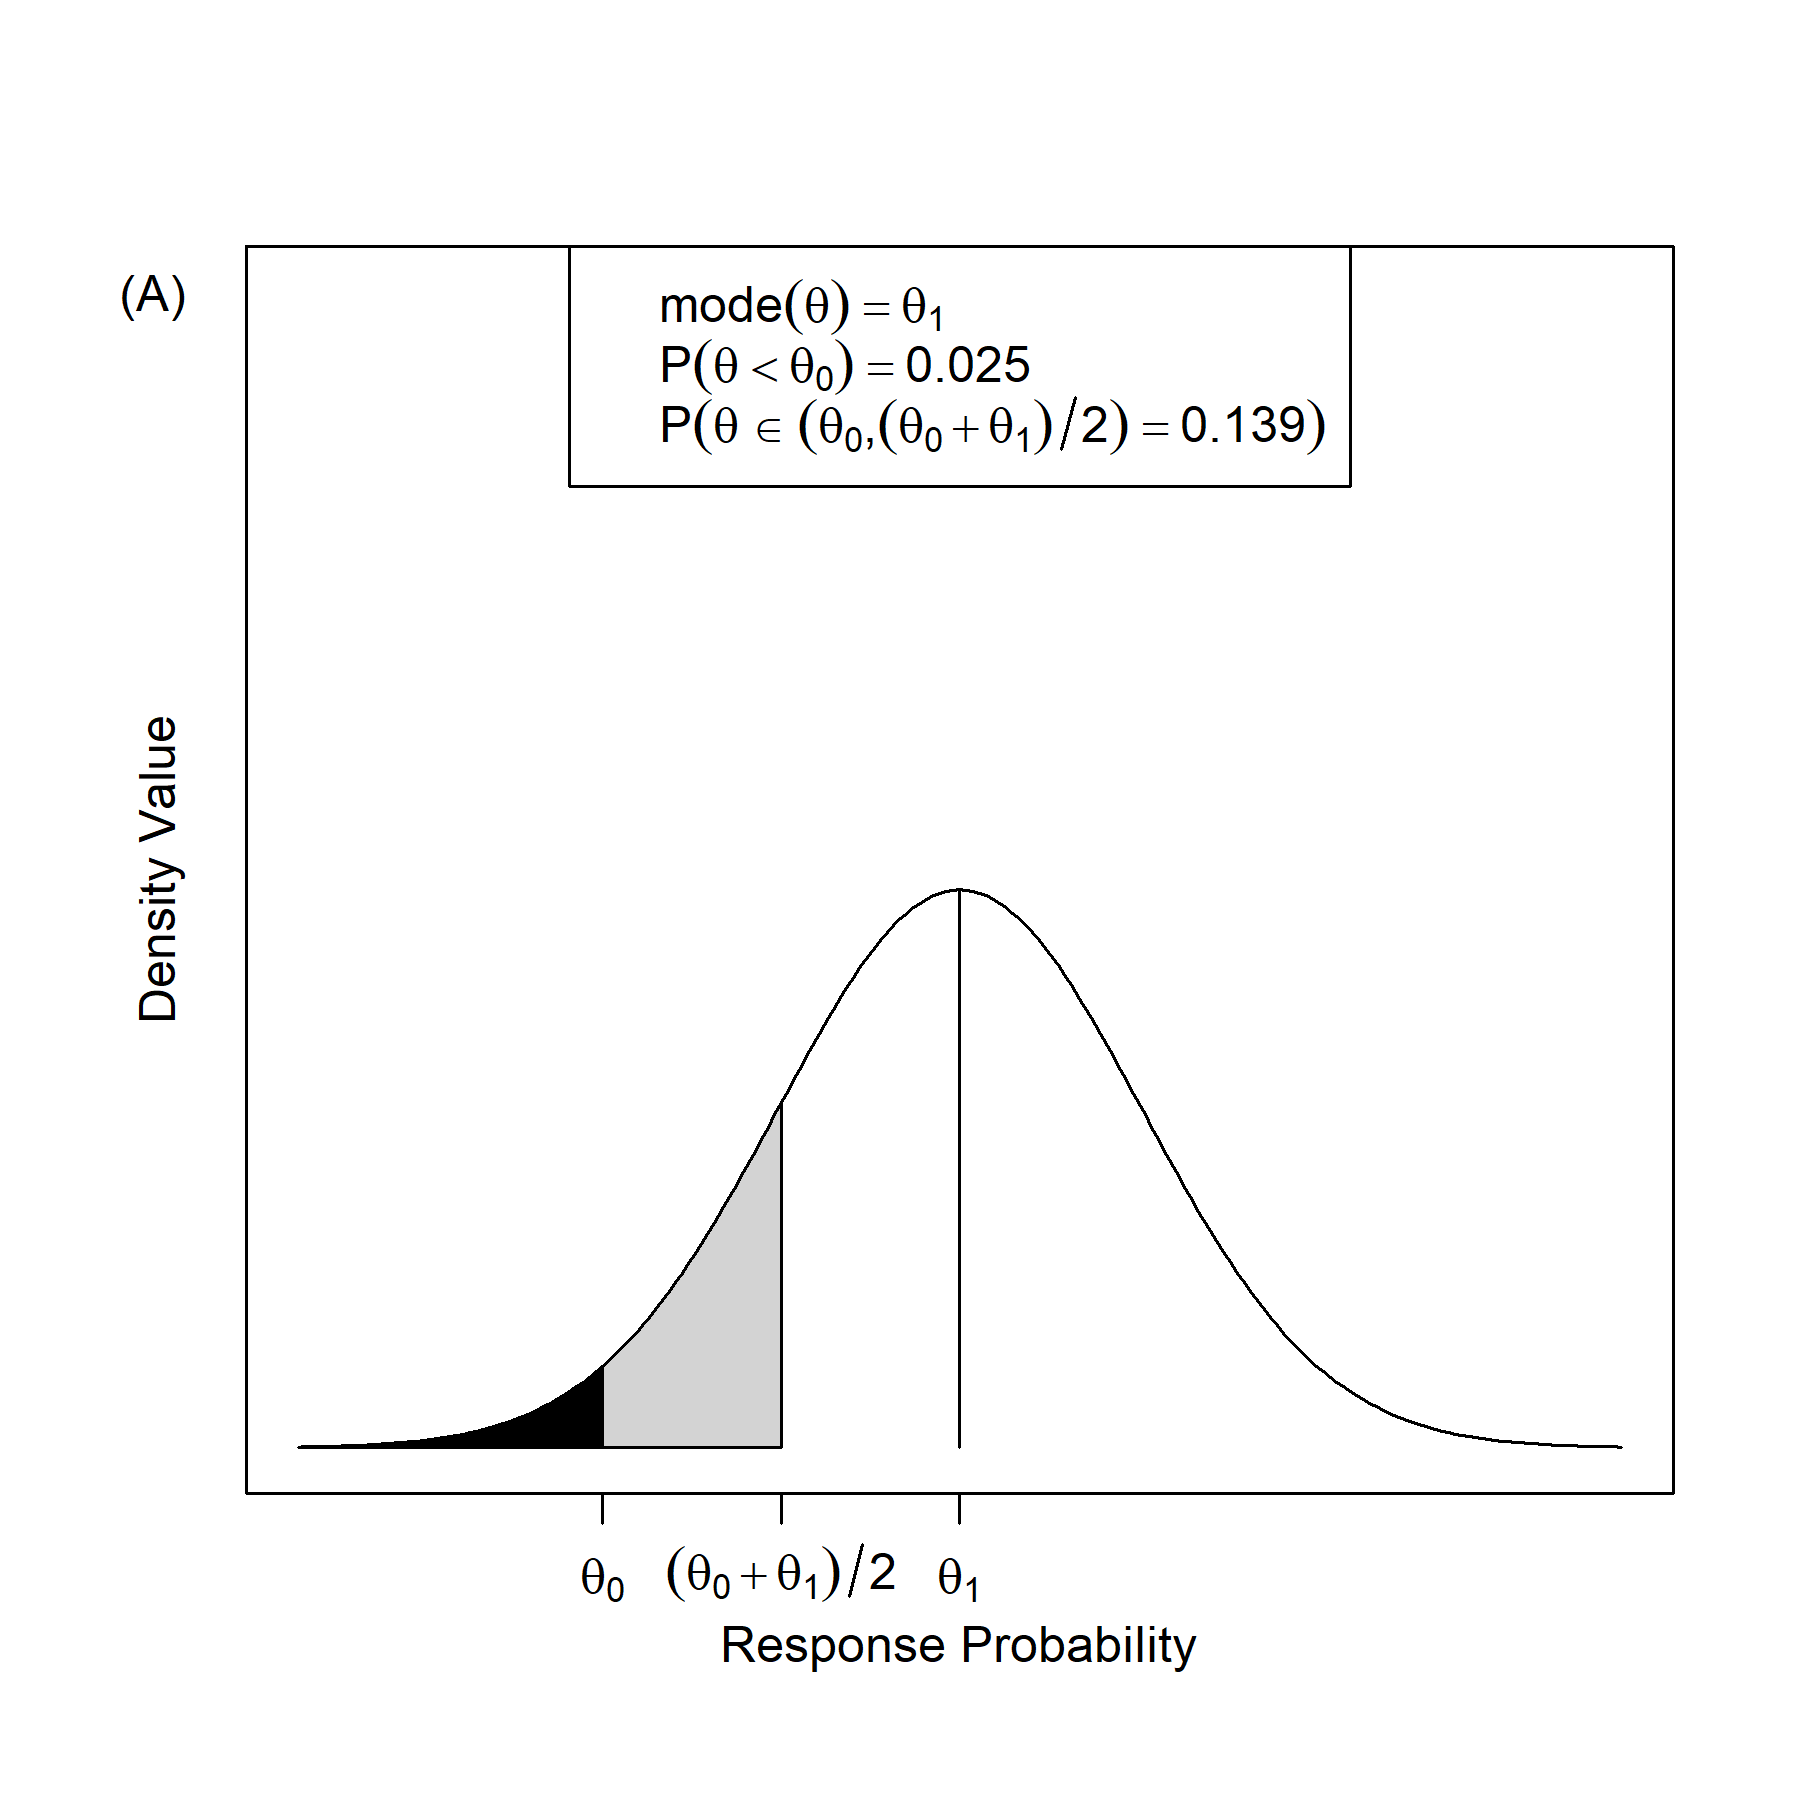
\includegraphics[width=3in]{P:/Bayesian-Sequential-Monitoring/00-paper/FIGURES/figure1a.png}
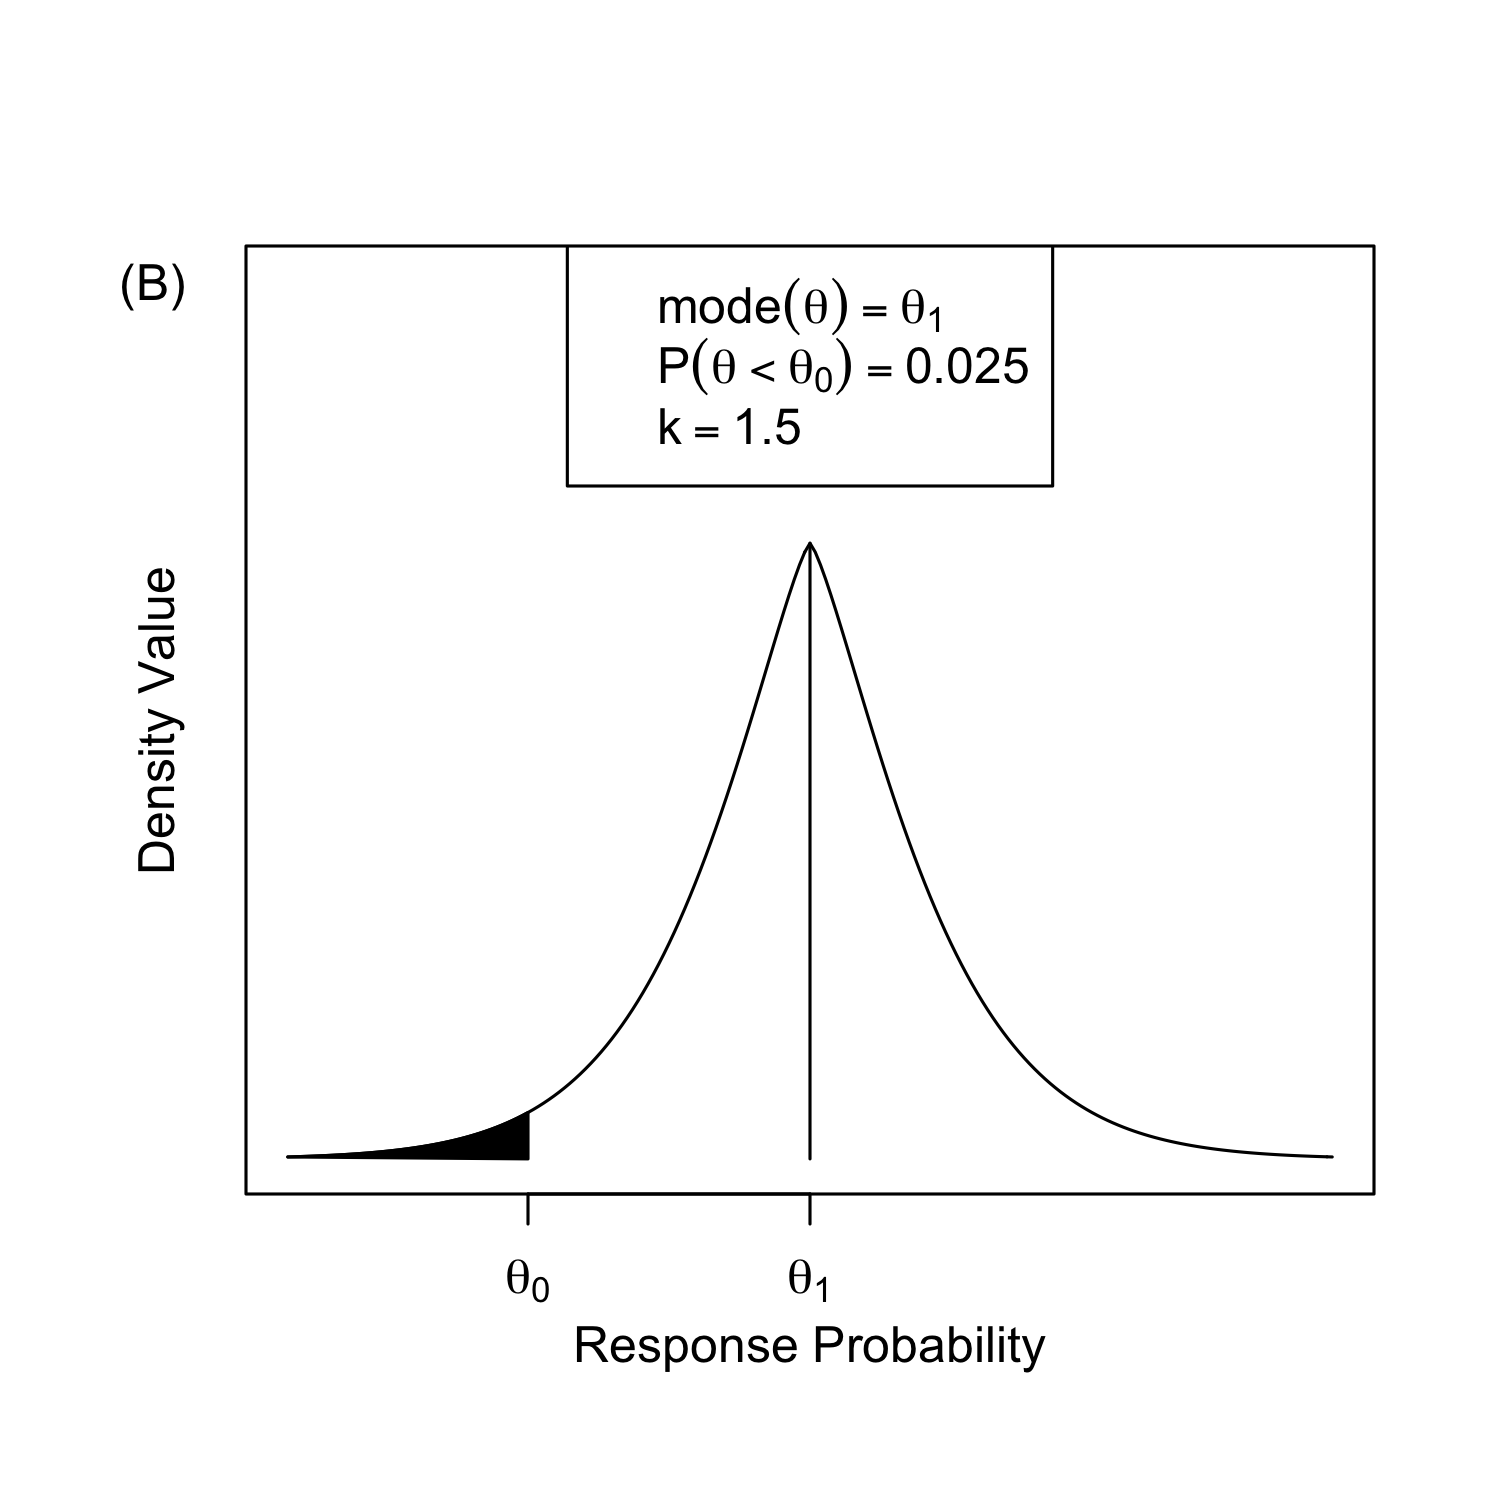
\includegraphics[width=3in]{P:/Bayesian-Sequential-Monitoring/00-paper/FIGURES/figure1b.png}

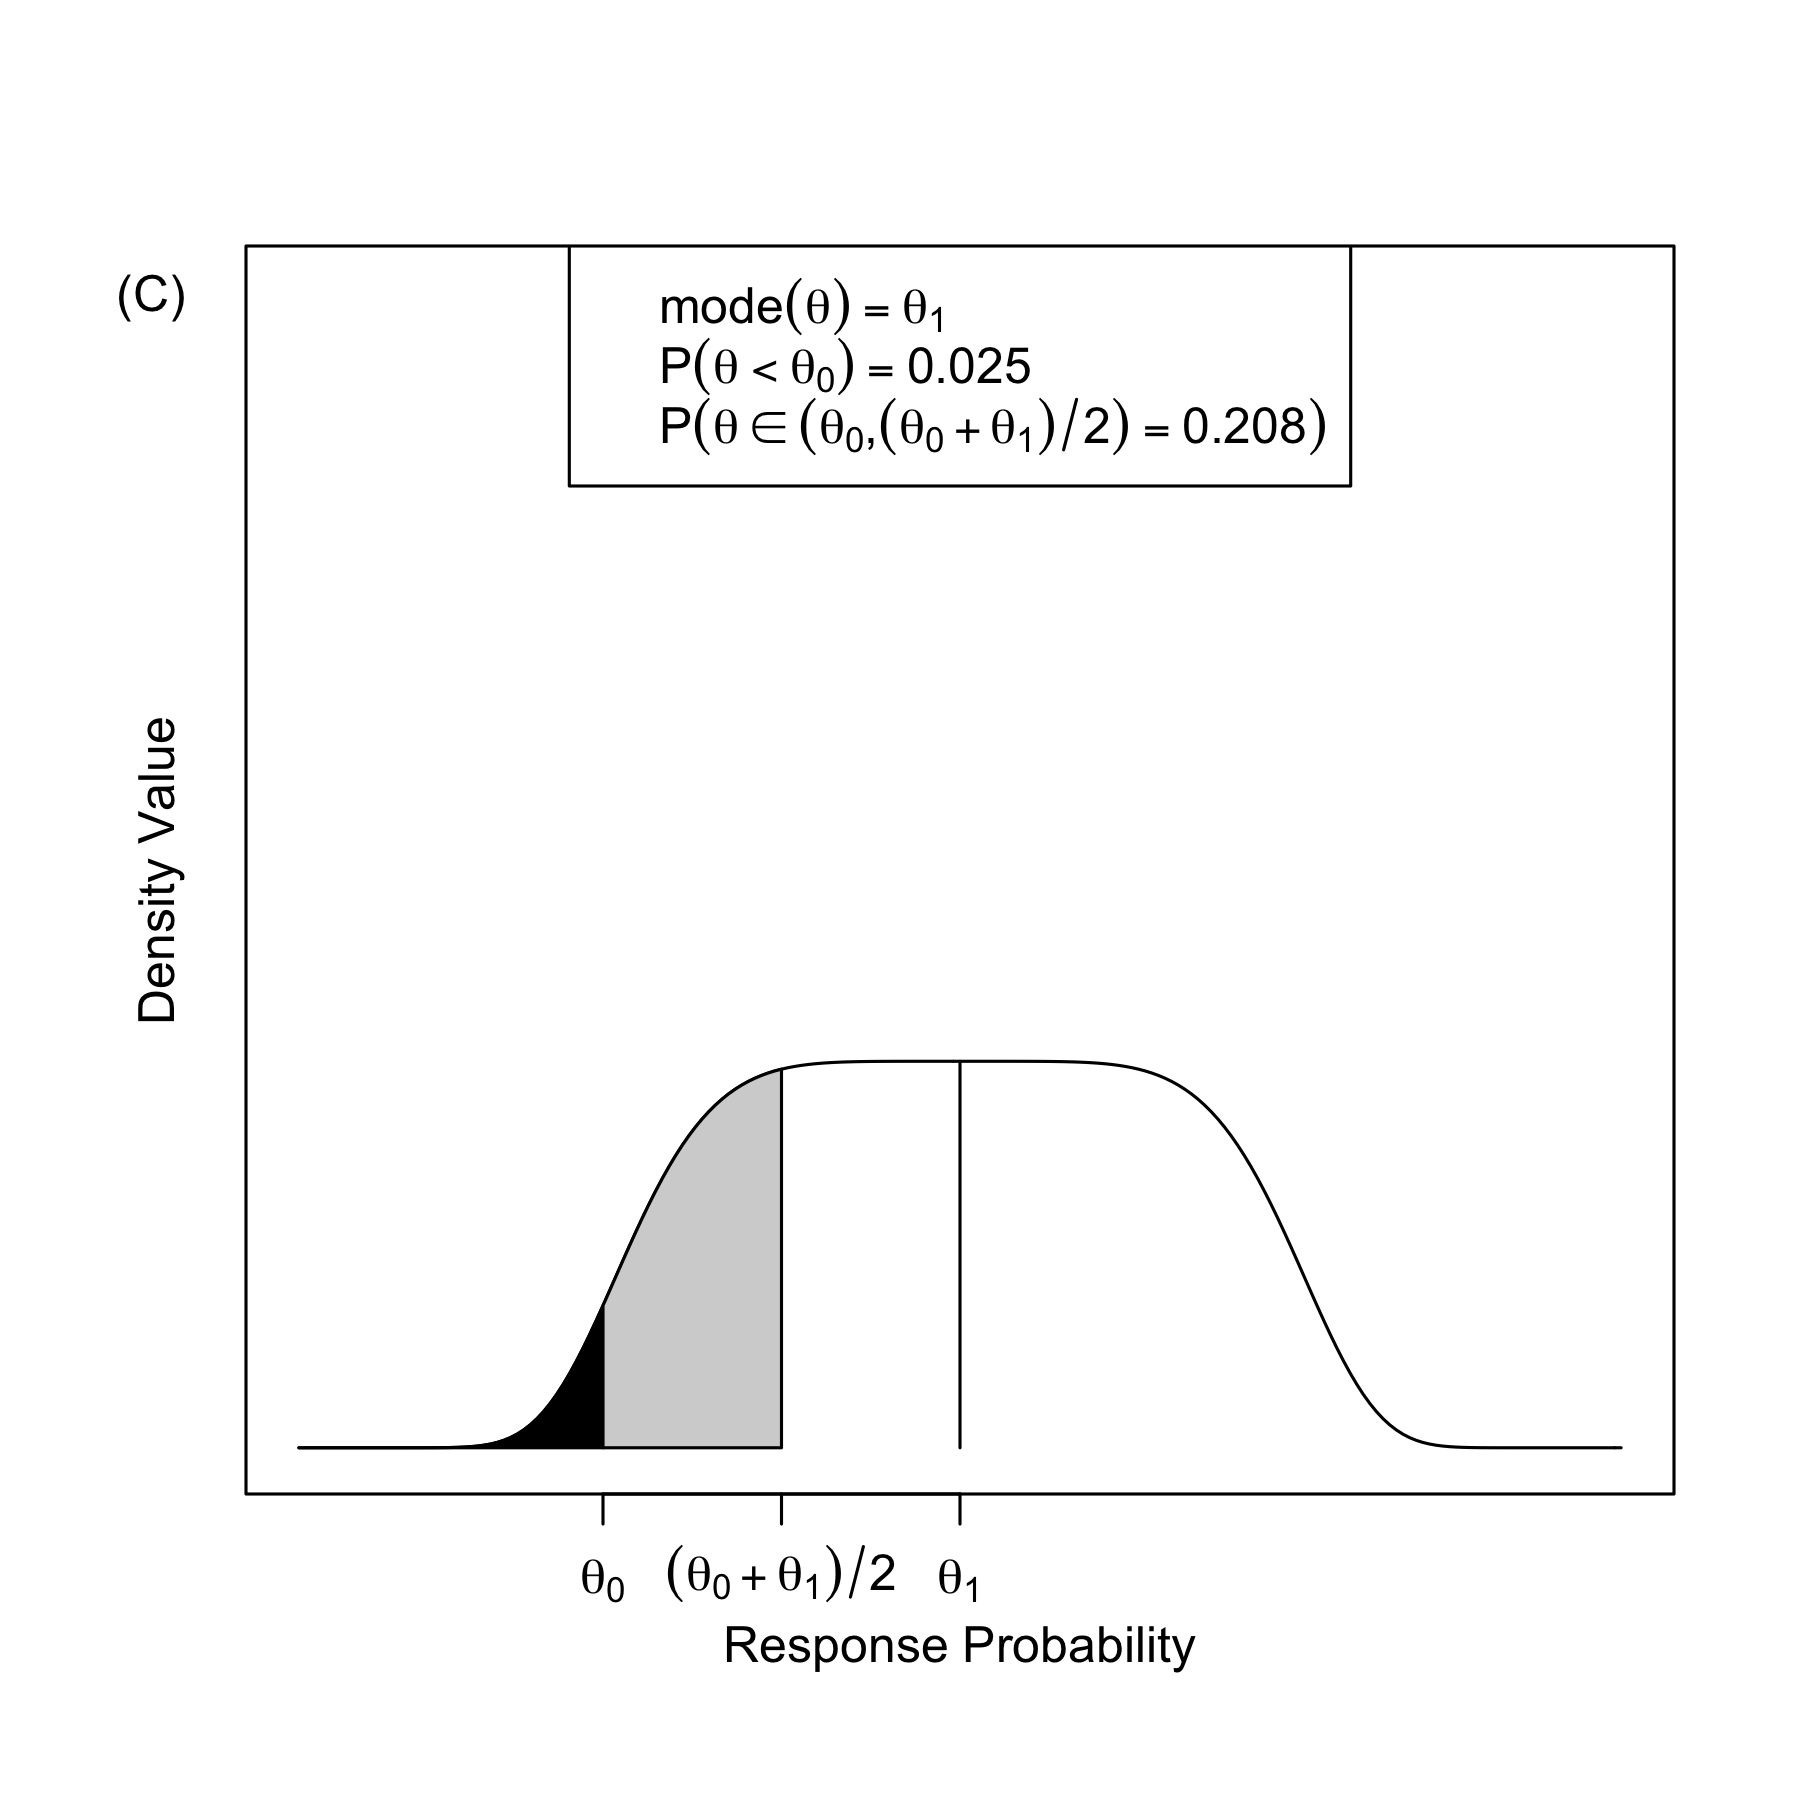
\includegraphics[width=3in]{P:/Bayesian-Sequential-Monitoring/00-paper/FIGURES/figure1c.png}
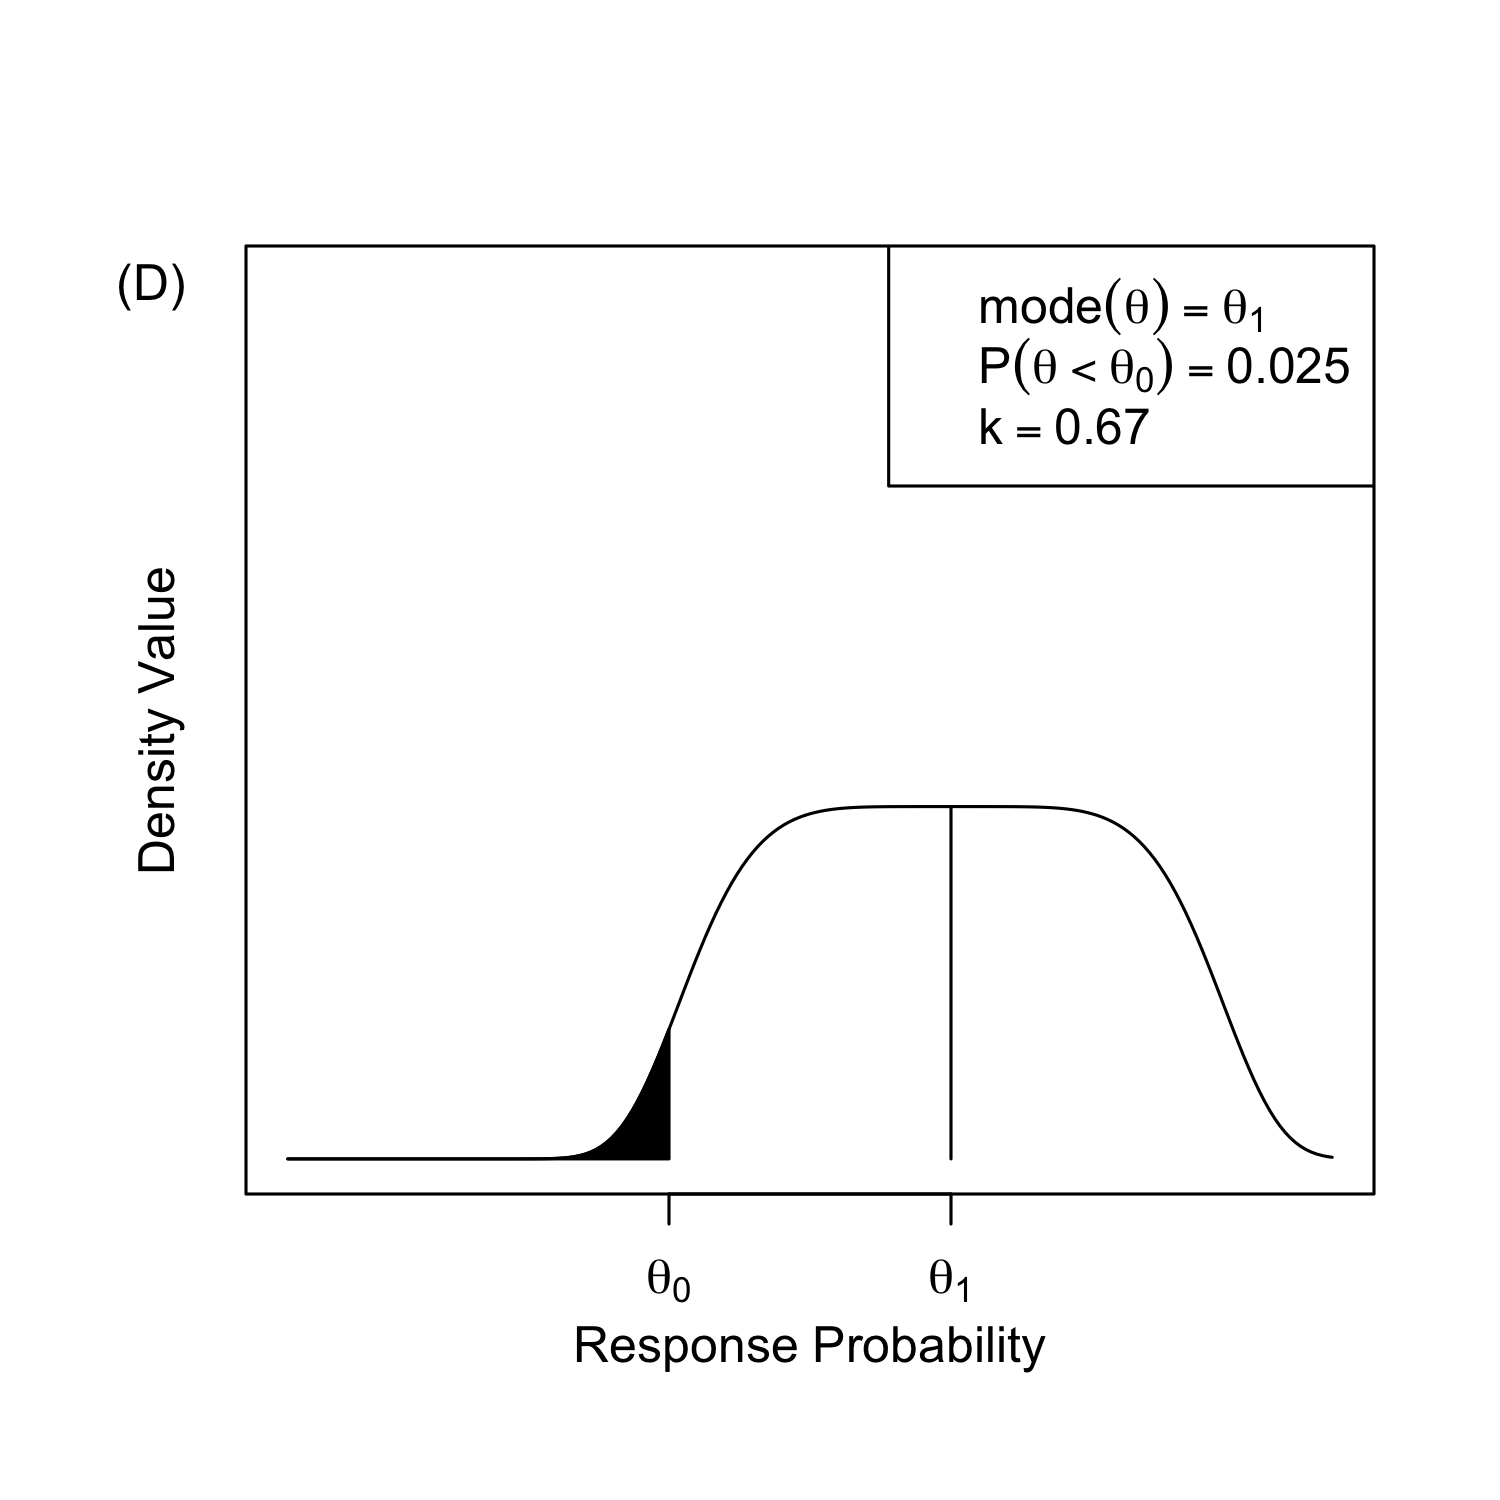
\includegraphics[width=3in]{P:/Bayesian-Sequential-Monitoring/00-paper/FIGURES/figure1d.png}

\caption{A, Skeptical prior, normal distribution. B, Skeptical prior, generalized normal distribution with added concentration around modal value. C, Enthusiastic prior, normal distribution. D, Enthusiastic prior, generalized normal distribution with added flattening around modal value.}
\label{fig:figure1}
\end{figure}

%
\subsubsection{Application to higher dimensions}
The generalized normal distribution can be used to parameterize skeptical and enthuastic priors for trials with multiple unknown quantities of interest. Suppose the trial from Section \ref{sec:preliminaries} has added a control arm, and let $\theta_0$ and $\theta_1$ be the response proportions for a control and treatment group respectively. Suppose that the risk difference $\theta_1-\theta_0$ is of interest. Let $\delta_{S}$ denote a null risk difference and $\delta_{E}$ denote a highly efficacious risk difference.


Consider the following representation of the joint prior for $\theta_1$ and $\theta_0$:
\begin{align}
\pi(\theta_0,\theta_1)=&\pi(\theta_0)\times\pi(\theta_1|\theta_0). \label{eq:generalized_normal_joint}
\end{align}

Each of these components can be represented in the form of (\ref{eq:generalizednormalkernel}) by
\begin{align}
\pi(\theta_0)\propto&\exp\left\{-\left(\frac{|\theta_0-\mu_0|}{\alpha_0}\right)^{\beta_0}\right\} \label{eq:generalized_normal_PC}\\
\pi(\theta_1|\theta_0)\propto&\exp\left\{-\left(\frac{|(\theta_1-\theta_0)-\delta|}{\alpha_1}\right)^{\beta_1}\right\}f(\theta_0). \label{eq:generalized_normal_IP}
\end{align}

The component $\pi(\theta_0)$ reflects prior opinion about the response rate in the placebo group, and the component $\pi(\theta_1|\theta_0)$ can be used to express pessimism or optimism in the difference in proportions $\theta_1 - \theta_0$. 

The enthusiastic prior condition from (\ref{eq:enthprior}) becomes
\begin{align}
P(\theta_1-\theta_0>\delta_S)=1-\epsilon.
\end{align}

The skeptical prior condition from (\ref{eq:skptprior}) becomes
\begin{align}
P(\theta_1-\theta_0<\delta_E)=1-\epsilon.
\end{align}


Examples of skeptical and enthusiastic priors are displayed in Figure \ref{fig:figure5}.

\begin{figure}
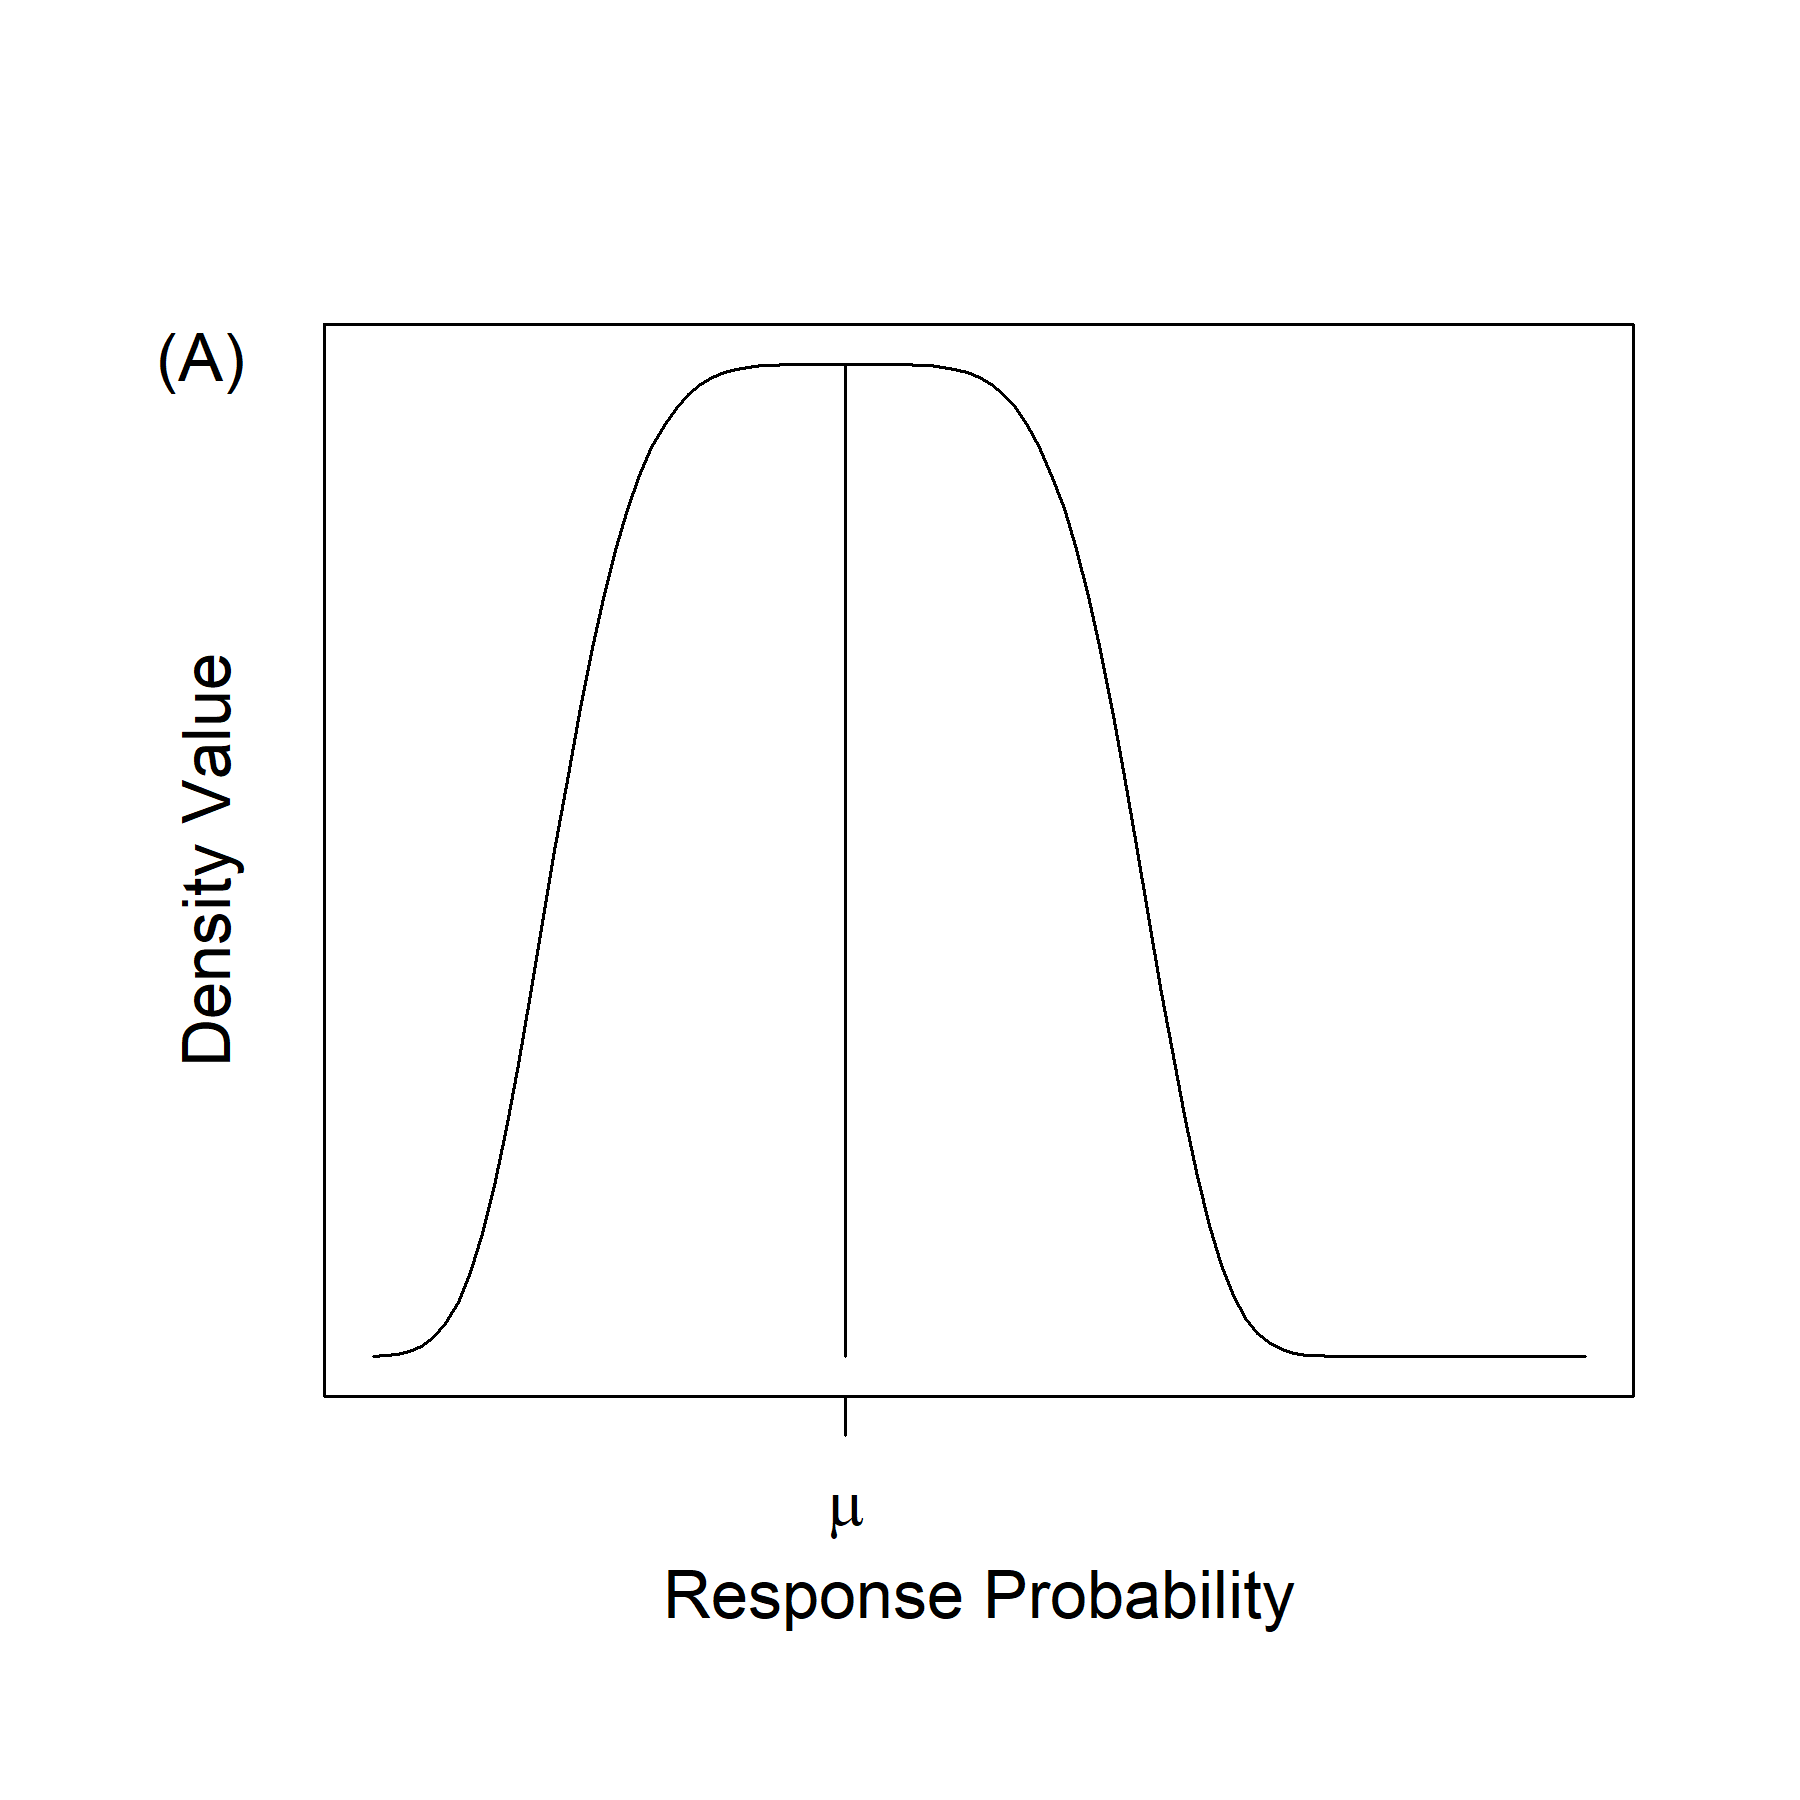
\includegraphics[width=3in]{P:/Bayesian-Sequential-Monitoring/00-paper/FIGURES/figure5c.png}

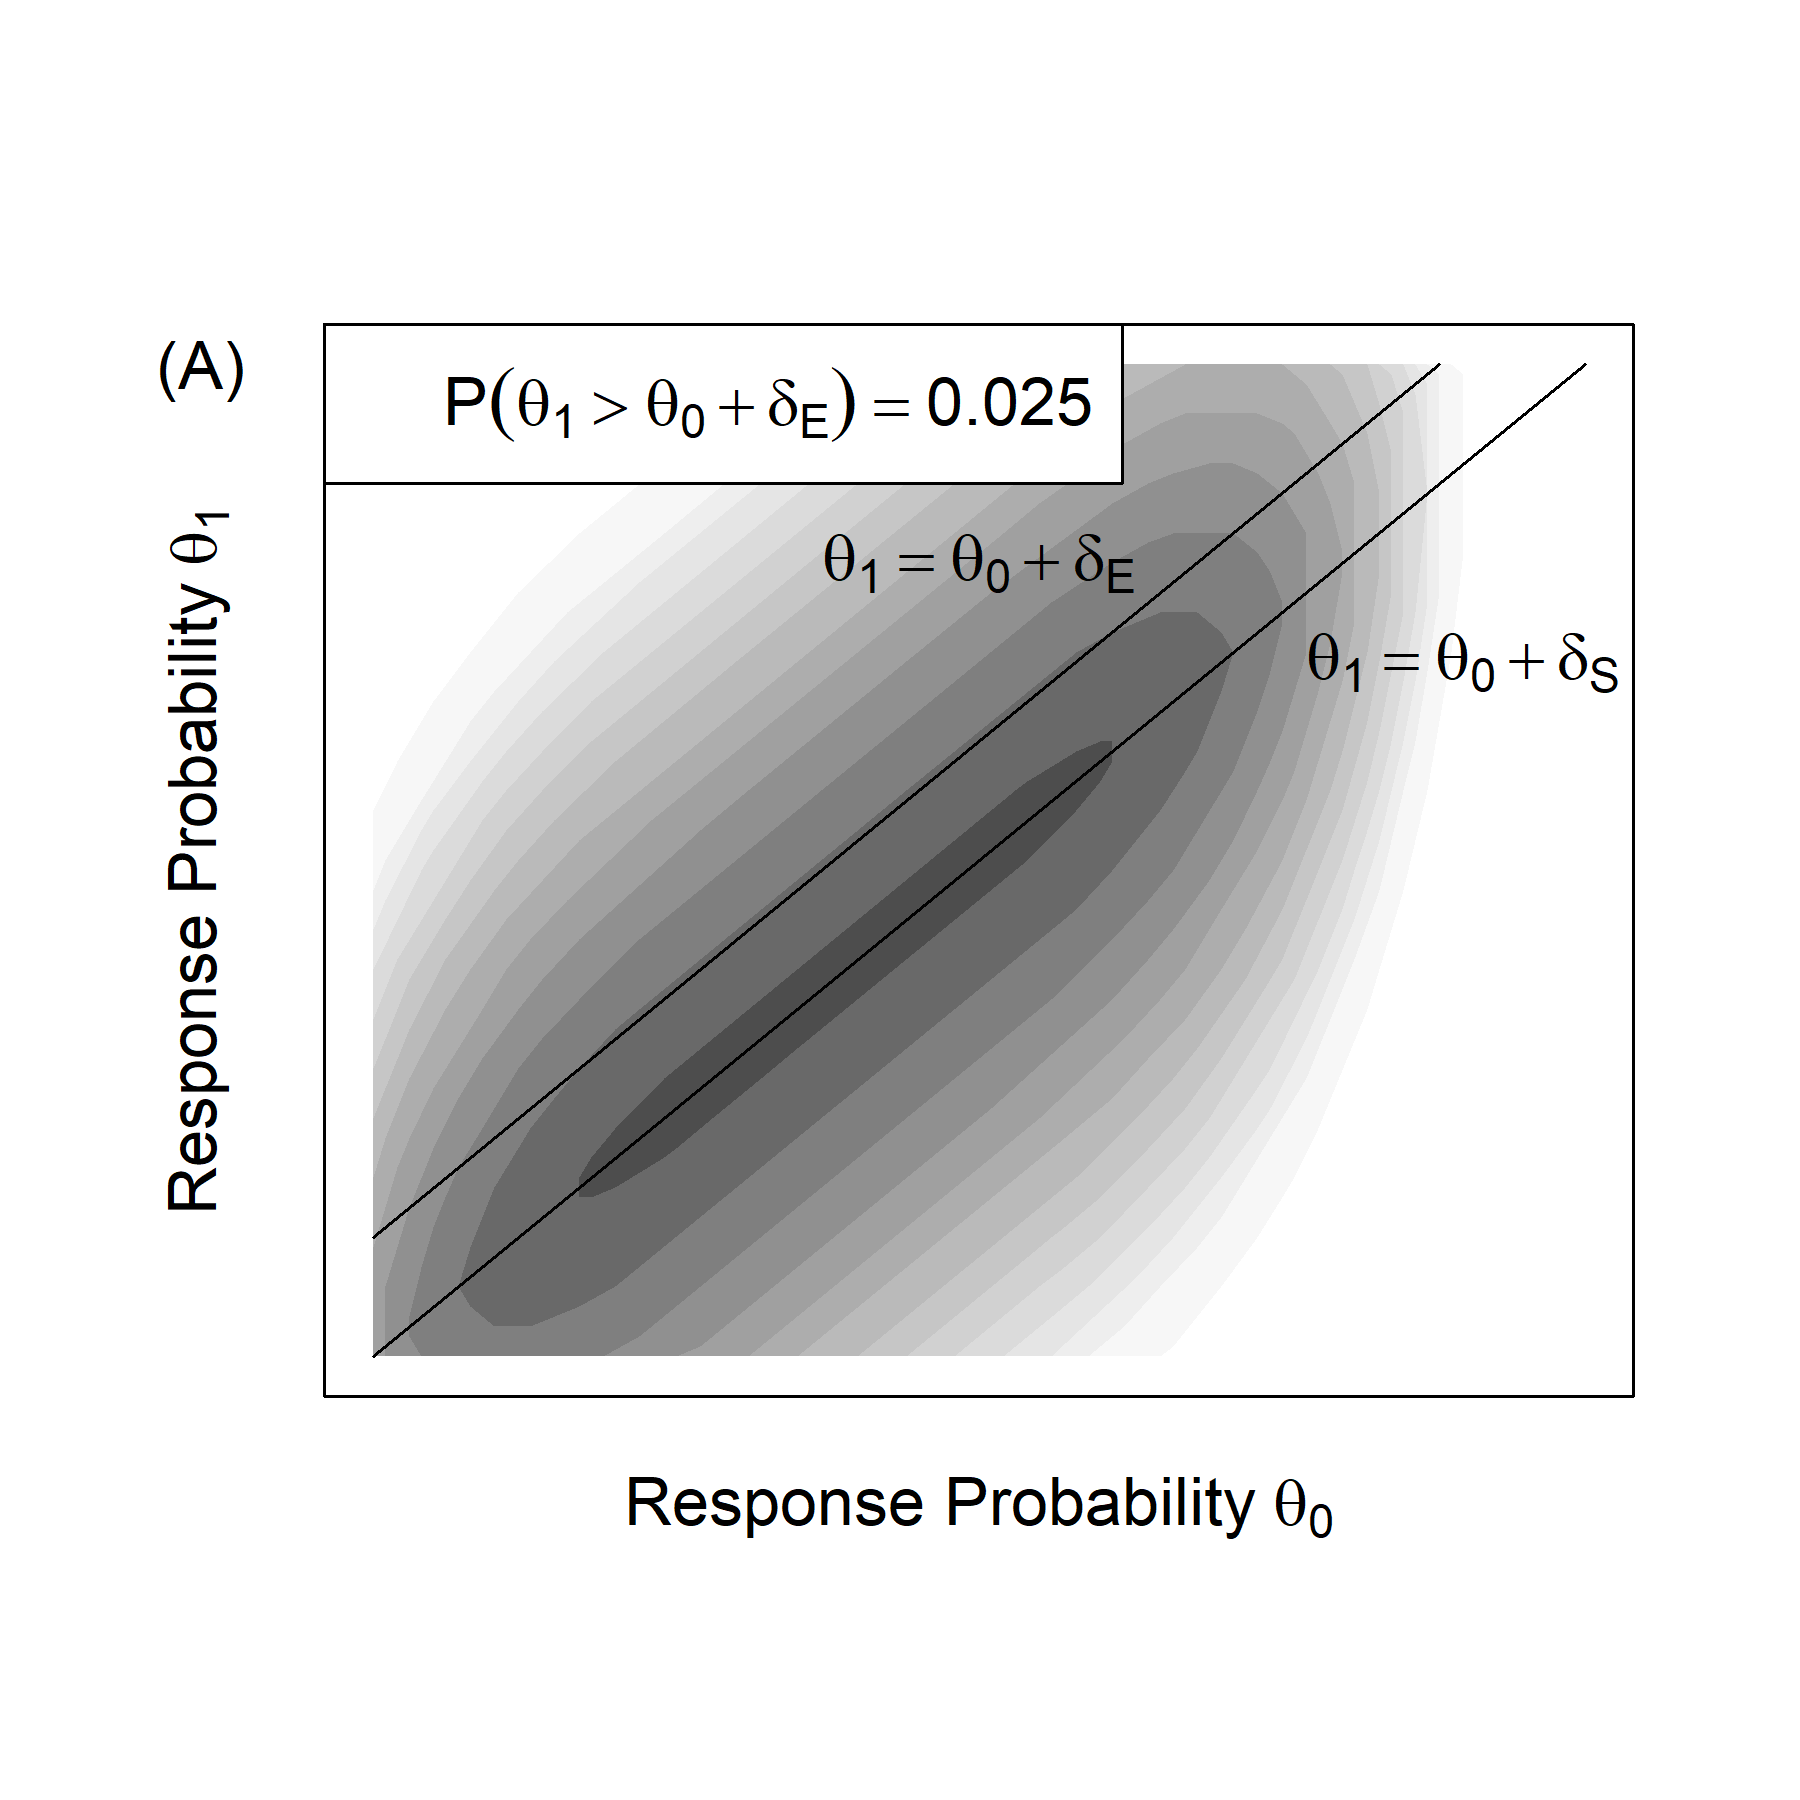
\includegraphics[width=3in]{P:/Bayesian-Sequential-Monitoring/00-paper/FIGURES/figure5a.png}
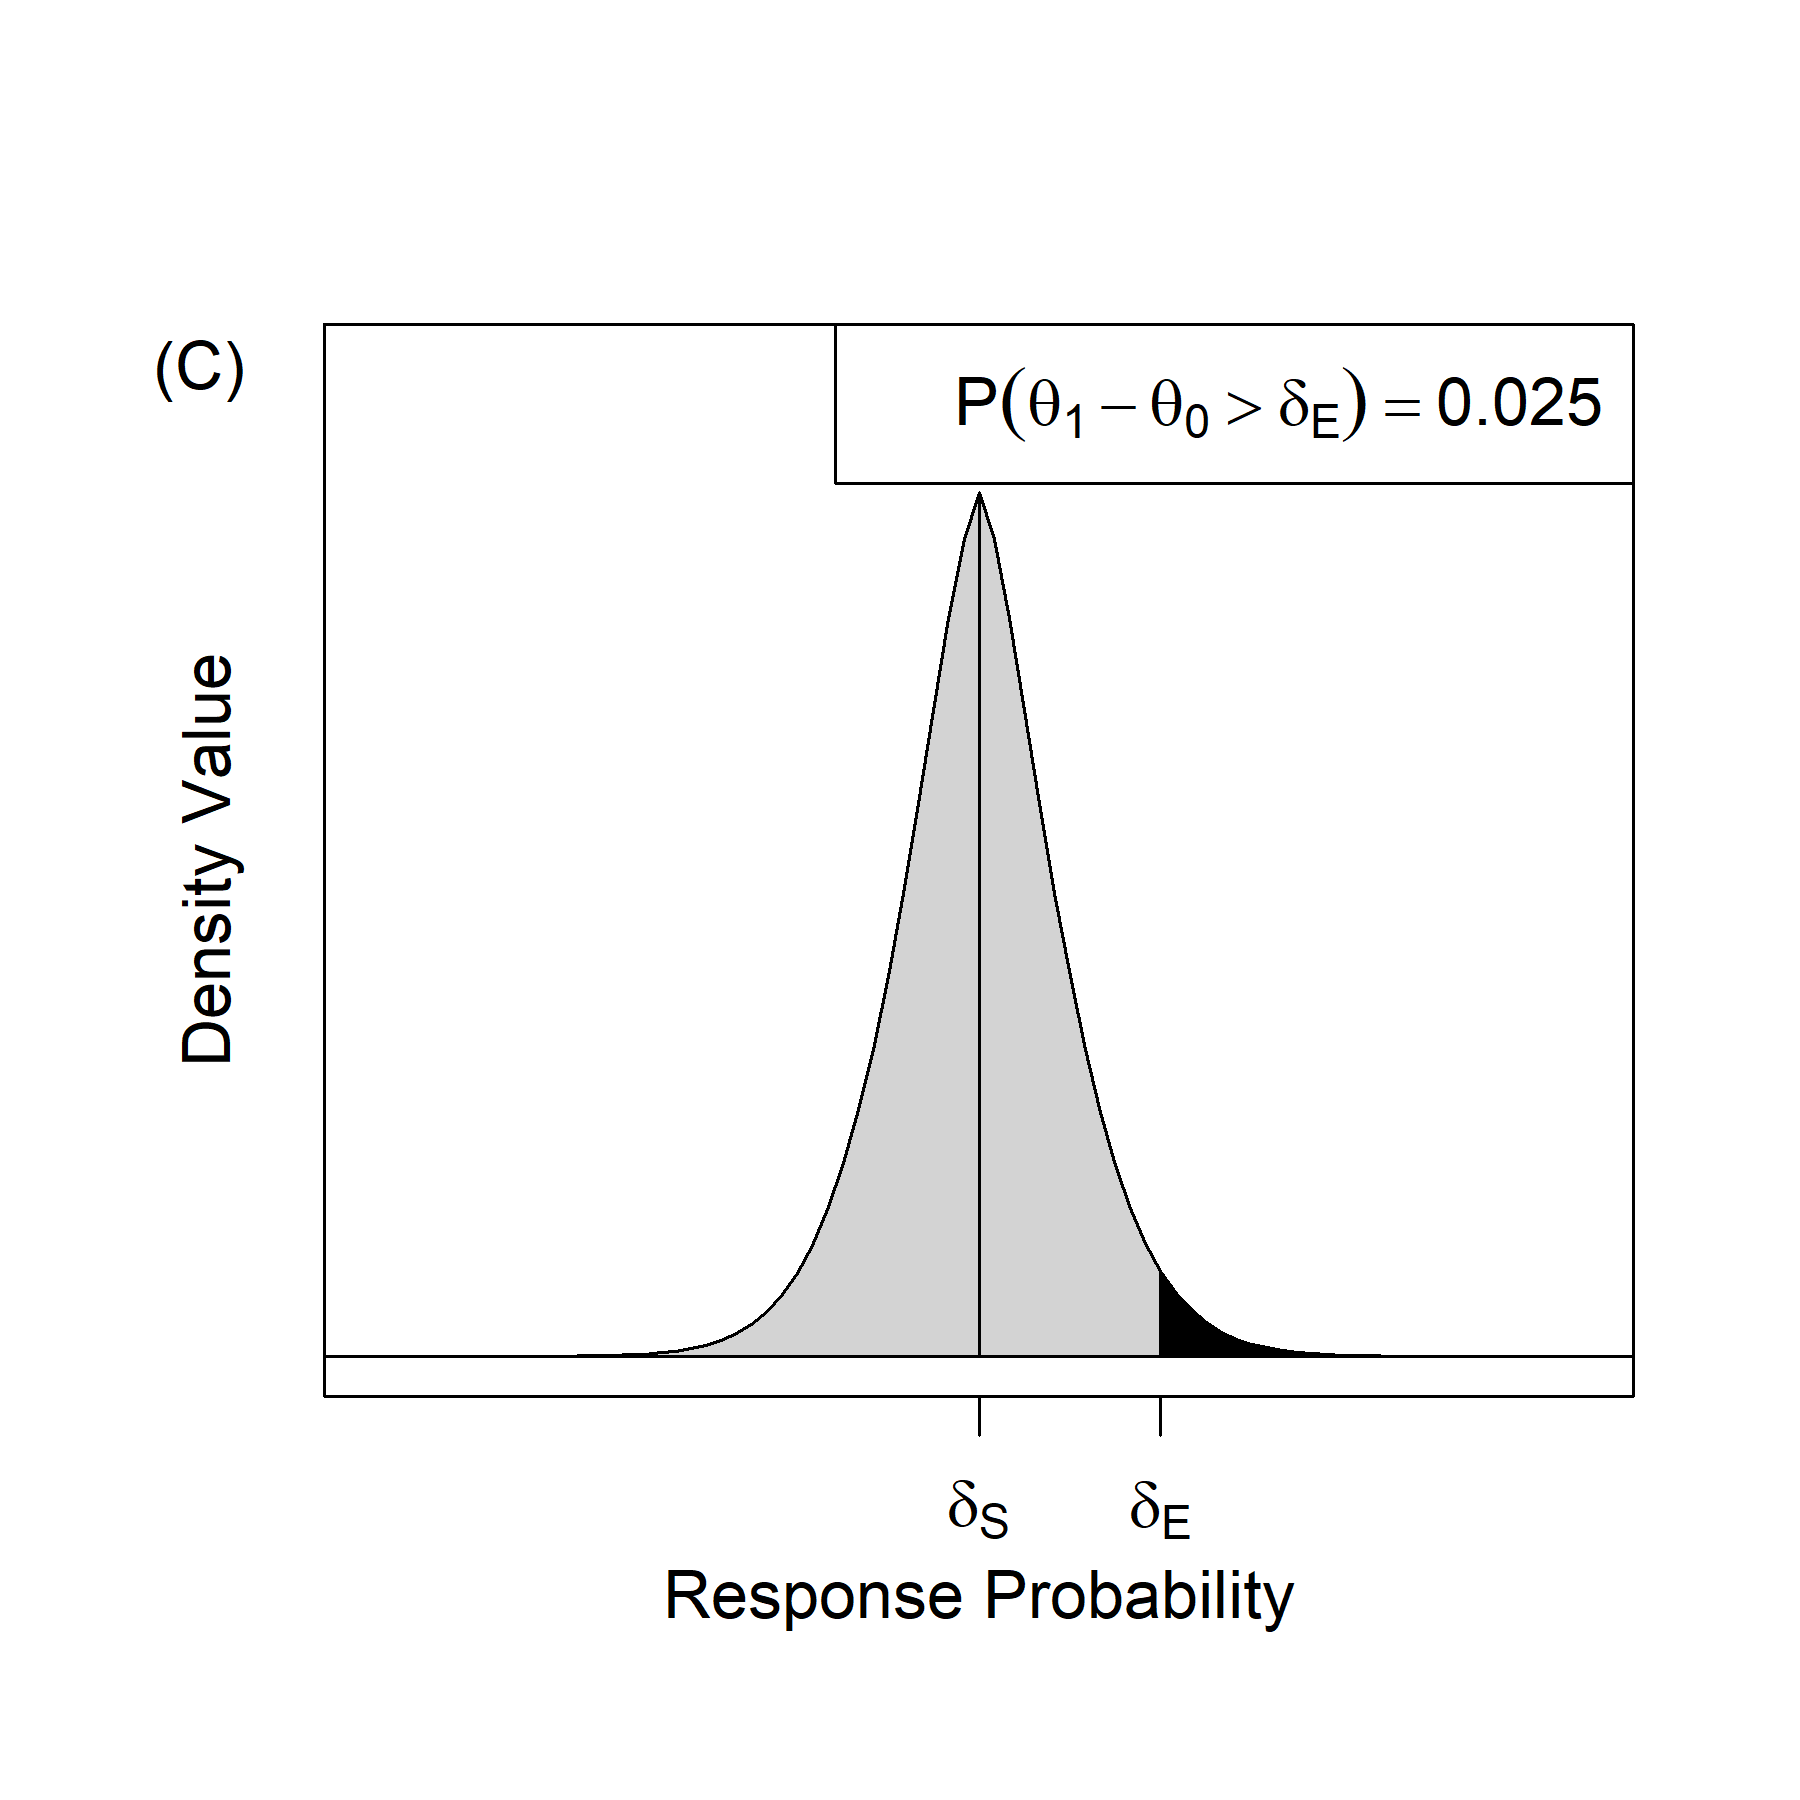
\includegraphics[width=3in]{P:/Bayesian-Sequential-Monitoring/00-paper/FIGURES/figure5d.png}

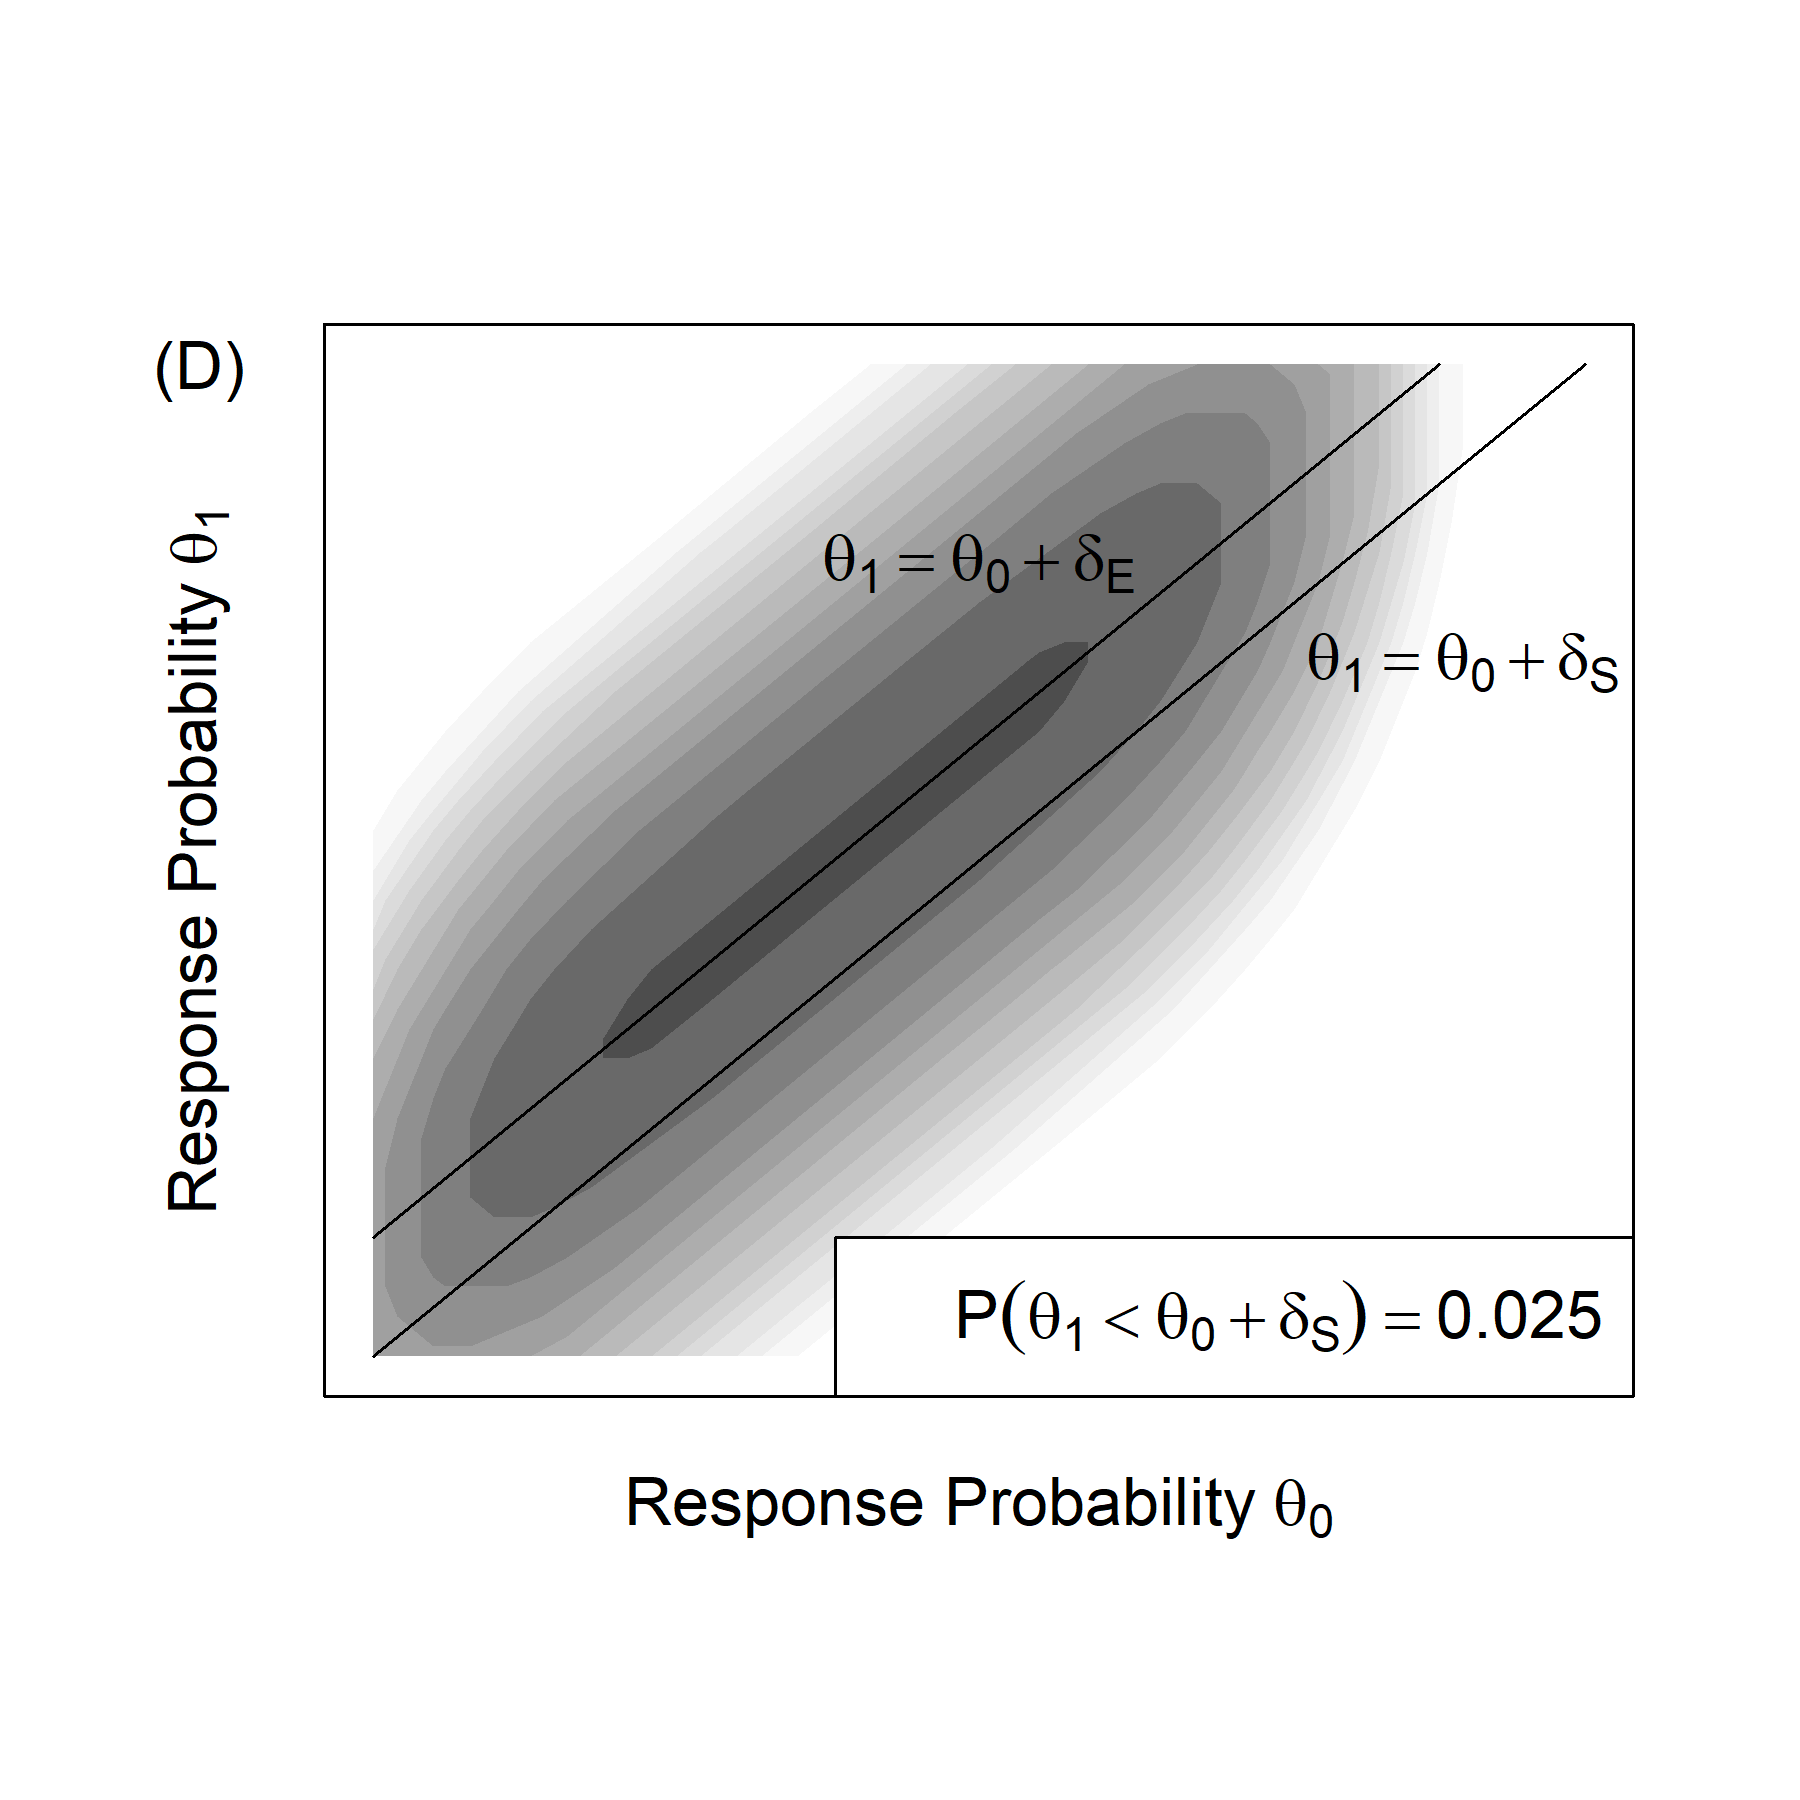
\includegraphics[width=3in]{P:/Bayesian-Sequential-Monitoring/00-paper/FIGURES/figure5b.png}
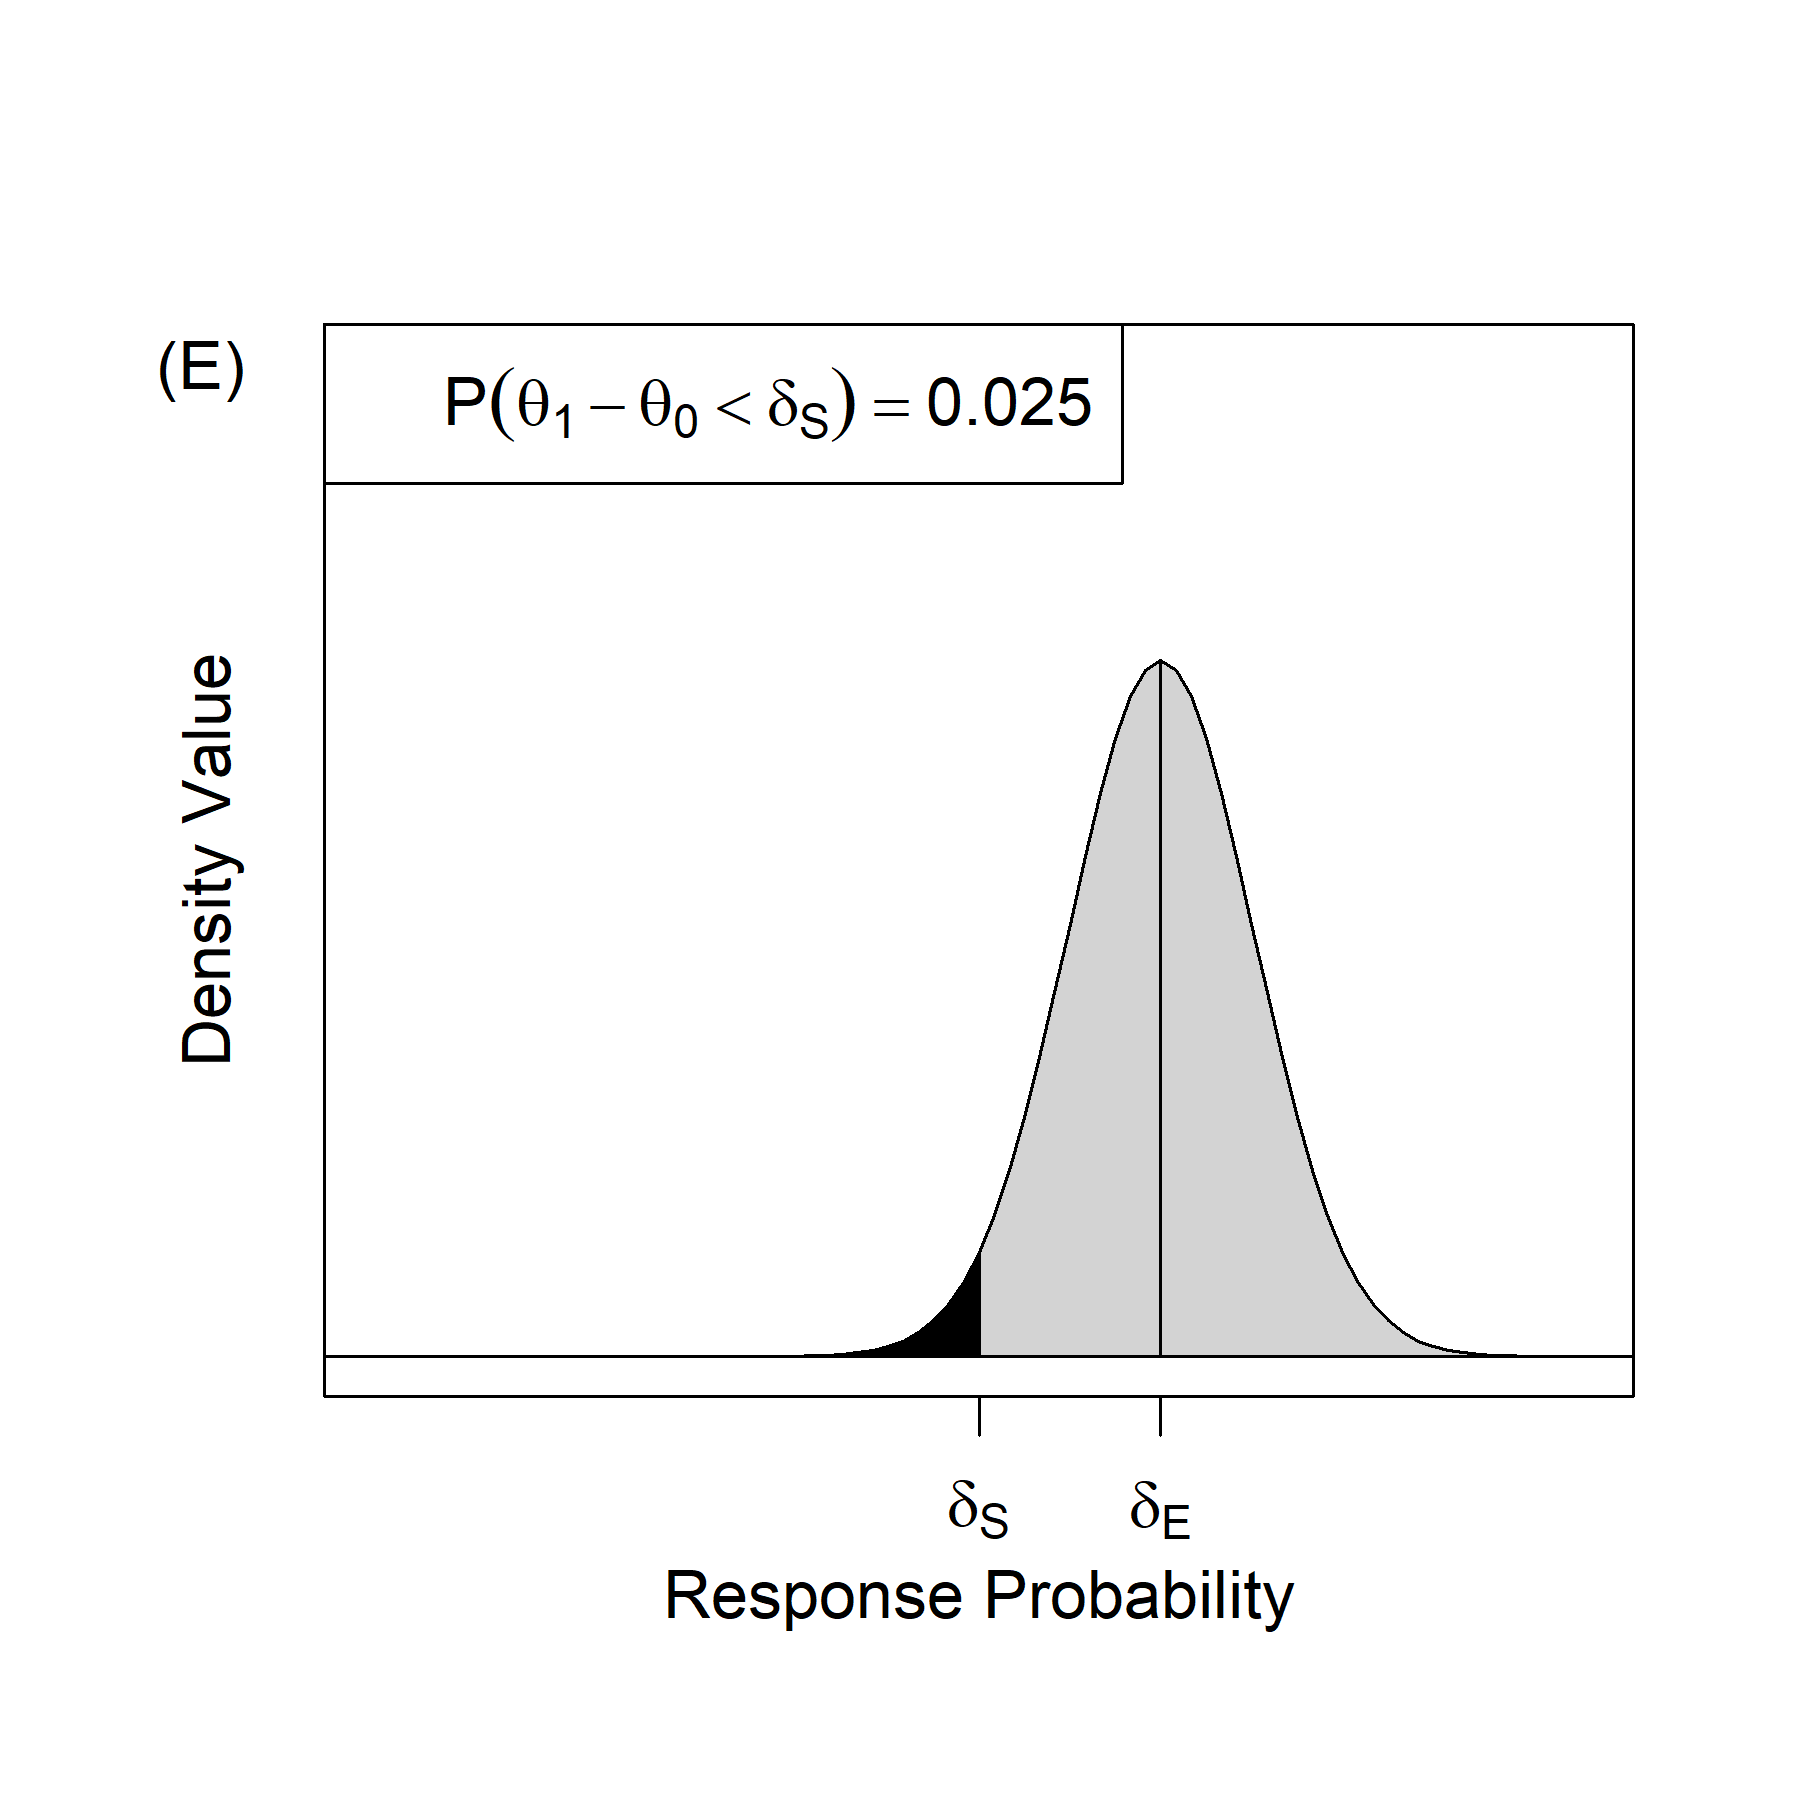
\includegraphics[width=3in]{P:/Bayesian-Sequential-Monitoring/00-paper/FIGURES/figure5e.png}
\caption{A, Prior on $\theta_1$. B, Skeptical joint prior. C, Skeptical marginal prior for $\theta_1-\theta_0$. D, Enthusiastic joint prior. E, Enthusiastic marginal prior for $\theta_1-\theta_0$.}
\label{fig:figure5}
 \end{figure}
\subsection{Mixture Inference Priors}
\subsubsection{Definition}
The purpose of the inference prior is to synthesize the posterior inferences from the a priori diverse perspectives to facilitate interpretation of the data once it has been obtained. In this paper we propose using an inference prior that is a combination of the skeptical and enthusiastic priors that were used for monitoring.

The skeptical and enthusiastic monitoring priors defined in Section~\ref{sec:MP} represent extreme but plausible beliefs about $\theta$.
%
While analysis with these priors provides a rational perspective from which one can determine whether interim data are sufficient 
to cease enrolling patients, the a priori belief of most stakeholders will likely fall somewhere in between.
%
Thus, when it interpreting the final data once in hand, intermediate perspectives should be considered.
%
To that end, we define an inference prior as a mixture prior constructed by mixing the monitoring priors.
%
Formally, the inference prior associated with mixing weight $\omega$ is given by
\begin{align}\label{eq:inference_prior}
\pi_{I}\left(\theta\right)=\omega\cdot\pi_{S}\left(\theta\right)+(1-\omega) \cdot \pi_E\left(\theta\right),
\end{align}
where $\omega\in[0,1]$. 
%
The specification of $\omega$ is done a priori, and the value $\omega=1/2$ will be referred to as an agnostic inference prior since it gives equal weight to the skeptical and enthusiastic prior.
%
%\textcolor{green}{
%If I'm not mistaken $\omega_0$ might be a better label for the prior mixing weight and then you could use $\omega\left(\mathbf{D}\right)$ in the expression
%below to represent the posterior mixing weight (which will depend on marginal likelihoods under the two priors). 
%%
%The notation $p(\pi_S|\mathbf{D})$ is not well-defined and will be confusing to reviewers. In my proposal you would use $\omega_0$.
%}
%%
%In particular,
%\begin{align}\label{eq:omega_formula}
%\omega=p(\pi_S|\mathbf{D})=\frac{p(\mathbf{D}|\pi_S)p(\pi_S)}{p(\mathbf{D}|\pi_S)p(\pi_S)+p(\mathbf{D}|\pi_E)p(\pi_E)}
%\end{align}
%where $p(\pi_S)+p(\pi_E)=1$. 
%%
%The quantities $p(\pi_E)$ and $p(\pi_S)$ reflect prior belief in the distribution of $\theta$. 
%%
%A default option is $p(\pi_S)=p(\pi_E)=\frac{1}{2}$. 

The distribution of $\theta$ using the inference 
prior, $p(\theta|\mathbf{D},\pi_I)$, will be used to compute summaries of $\theta$ such as the posterior mean and quantiles. The posterior distribution for $\theta$ using (\ref{eq:inference_prior}) is
\begin{align}
p(\theta|\mathbf{D},\pi_I)&=\hat{\omega}\cdot p(\theta|\mathbf{D},\pi_S)+(1-\hat{\omega})\cdot p(\theta|\mathbf{D},\pi_E)
\end{align}
where the updated mixing weight is
\begin{align}
\hat{\omega}&=\frac{\omega\cdot p(\mathbf{D}|\pi_S)}{\omega\cdot p(\mathbf{D}|\pi_S)+(1-\omega)\cdot p(\mathbf{D}|\pi_E)}
\end{align}
where $p(\mathbf{D}|\pi_S)=\int p(\mathbf{D}|\theta)\pi_S(\theta)d\theta$ and $p(\mathbf{D}|\pi_E)=\int p(\mathbf{D}|\theta)\pi_S(\theta)d\theta$. 

%
%Choosing $\omega=1/2$ for an equal mixture of $\pi_S$ and $\pi_E$ corresponds to an inference prior that equally weights the skeptical and enthusiastic opinions. Define $p(\mathbf{D}|\pi(\theta))=\int p(\mathbf{D}|\theta)\pi(\theta)d\theta$ to be the marginal likelihood for the data given the prior $\pi(\theta)$. Choosing $\omega$ based on posterior model probabilities of the null and alternative hypotheses yields 
%\begin{align}
%\omega=\frac{p(\mathbf{D}| \pi_{S})}{p(\mathbf{D}| \pi_{S})+p(\mathbf{D}| \pi_{E})}. 
%\end{align}
%The determination of a significant trial result is given by
%\begin{align*}
%P(\theta\in\Theta_1|\mathbf{D},\pi_I)\geq\delta.
%\end{align*} 

%All relevant information about $\theta$ can be derived from the marginal posterior distribution with an inference prior (e.g. posterior mean, credible intervals). For example, the posterior mean using the inference prior will be a two-part mixture of the posterior means using the skeptical and enthusiastic priors: $E(\theta|\mathbf{D},\pi_I)=\omega E(\theta|\mathbf{D}, \pi_{S})+(1-\omega) E(\theta|\mathbf{D}, \pi_{E}).$
\subsubsection{Incorporating Prior Information in the Monitoring Priors}
The skeptical and enthusiastic monitoring priors can be viewed as a weighted combination such as in the inference prior (\ref{eq:inference_prior}) with weights $\omega=1$ and $\omega=0$ respectively. This weighted combination can be used as a replacement for the monitoring prior for any fixed weight $\omega$. For example, a ``not-as-skeptical" prior can be defined as $\tilde{\pi_S}(\theta)=0.75\cdot\pi_S(\theta)+0.25\cdot\pi_E(\theta)$. 

Alternatively, $\omega$ can be informed by the data. Let $\hat{\theta}=argmax \{p(\mathbf{D}|\theta)\}$ be the maximum likelihood estimator of $\theta$ given the data. Define
\begin{align}
\omega=\frac{\pi_S(\hat{\theta})}{\pi_S(\hat{\theta})+\pi_E(\hat{\theta})}
\end{align}
as a mixing weight that dynamically gives preference to the prior that has the higher density evaluated at $\hat{\theta}$.
%\textcolor{green}{We don't have anything in the paper about using a mixture of the skeptical and enthusiastic prior to 
%define a ``less'' skeptical monitor prior that incorporates information from another source using the 
%notion of applicability (i.e., a fixed value of $\omega_0$ that is not 1.). 
%%
%This is fundamental to the novelty of the paper. 
%%
%I think it would be good to show how the GN can be used to inform a prior for the control group with flexibility here (e.g., flattening the prior over an interval)
%AND talking about the mixture skeptical monitoring prior.
%%
%In the case of using ``no prior information'' the enthusiastic prior is simply used for monitoring. But it can be incorporated directly into the 
%skeptical prior when it is informed by data using the concept of applicability.
%%
%Isn't that what was done for the second example? Lets talk if we need to. This is a big part of the novelty.
%}

%\\
%\int_\Theta \theta p(\theta|\mathbf{D},\pi_{I})d\theta&=\omega\cdot \int_\Theta \theta p(\theta|\mathbf{D},\pi_{S})d\theta+(1-\omega)\cdot\int_\Theta \theta %p(\theta|\mathbf{D},\pi_{E})d\theta
%\begin{align*}
%\pi_{Inference}=\frac{p(\mathbf{D}| \pi_{S}) \pi_{S}+p(\mathbf{D}| \pi_{E}) \pi_{E}}{p(\mathbf{D}| \pi_{S})+p(\mathbf{D}| \pi_{E})}
%\end{align*}
%\begin{align*}
%E(\theta|\mathbf{D},\pi_{Inference})=\omega\times E(\theta|\mathbf{D}, \pi_{S})+(1-\omega)\times E(\theta|\mathbf{D}, \pi_{E})
%\end{align*}
%Need to describe relation to Type I and Type II error.
%\subsubsection{Default parameterization of monitoring priors for common designs}\label{monitoring_prior_specification}
%Define prior distribution as $\pi(\theta|\lambda)$ where $\lambda$ is a vector of hyperparameters.

%Reference prior attempts to express no particular opinion about the treatment's merit. 

\section{Examples}

\subsection{Single-Arm Proof-of-Activity Trial with Binary Endpoint}
\subsubsection{Motivating example}
\textcolor{green}{You need more details on the motivating example. Describe the trial, cite papers about the trial. 
%
The current writeup leaves out way to much background.
%
What was the outcome -- currently the writeup does not even say? At what time point was the primary outcome assessed?
%
Start by describing the trial(s) pediatric and adult that are used for this motivation. 
%
That should come first. If that is done adequately the first paragraph below will be unneeded as it will have been made clear by the motivating example description.
}

Consider a single-arm proof-of-activity trial with a binary endpoint. The data $\mathbf{D}$ are binomially distributed and the response rate $\theta$ is the parameter of interest, with higher values of $\theta$ being indicative of proof-of-activity. 

An example application is based on the drug iniximab, which is FDA approved for the treatment of several diseases, including ulcerative colitis (UC). The goal of the trial is to test the hypothesis: $H_0:\theta\leq\theta_0=0.40$ versus $H_1:\theta>\theta_0$. From adult data $\theta_1=0.67$. Based on the 54-week follow-up period, we can infer enrollment took place over approximately 33 months (approximately 1 patient per 0.55 months).

\subsubsection{Model formulation \& prior elicitation}
The default skeptical and enthusiastic priors will be of the form (\ref{eq:generalizednormalkernel}) with $\beta=2$ corresponding to truncated normal distributions
\begin{align}
\pi_S(\theta)&\propto \exp\left\{-\frac{(\theta-\theta_0)}{\alpha_S}^2\right\} I(\theta\in[0,1])\\
\pi_E(\theta)&\propto \exp\left\{-\frac{(\theta-\theta_1)}{\alpha_E}^2\right\} I(\theta\in[0,1])
\end{align}
with $\alpha_S$ and $\alpha_E$ chosen satisfy (\ref{eq:enthprior}) and (\ref{eq:skptprior}) with $\epsilon=0.025$.

\textcolor{green}{All figures should be referenced in text and discussed.}


 

The following illustrations and analyses were performed using the concentrated skeptical prior and the default enthusiastic prior.
\textcolor{green}{Question from reviewer: Then why are the others shown? Why are you recommending practitioners use these? Are results for other combinations somewhere?
%
If so, you should have: A comparison of the various combinations of the monitoring priors in Figure~\ref{f:figure1} is provided in Supplemental Appendix X.}
\subsubsection{Sequential monitoring}
Enrollment will proceed until one of the following three conditions are satisfied:
\begin{align*}
\text{Efficacy criteria (EFF): }&P(\theta>\theta_0|\mathbf{D},\pi_S)\geq 0.975\\
\text{Futility criteria (FUT): }&P\left(\theta\leq\frac{\theta_0+\theta_1}{2} \Big|\mathbf{D},\pi_E\right)\geq 0.975\\
\text{Maximum sample size: }&N=112 \text{ patient outcomes obtained}
\end{align*}

(describe reason for maximum sample size)

Assume that the outcomes are ascertained after approximately 4 months of follow-up and 2 patients per month on average are enrolled. If enrollment is terminated due to the efficacy or futility criteria being satisfied, those subjects who are still undergoing follow-up will still have their outcomes considered in the final analysis. (describe enrollment and follow-up distributions used in the simulations)

\subsubsection{Example paths}
Figure \ref{fig:figure2a} shows the results of a hypothetical trial with the initial prior specification (first panel), three interim analyses (middle panels), and a final analysis (last panel).

Old write-up below: needs to be updated:

As seen in Figure 3(a), at the second interim analysis the efficacy condition $P(\theta>0.20|\mathbf{D},\pi_S)\geq 0.95$ is satisfied and enrollment is terminated. As shown in Figure 3(b), at the fourth interim analysis the futility condition $P(\theta\leq 0.30|\mathbf{D},\pi_E)\geq 0.85$ is satisfied and enrollment is terminated. In both examples there are subjects with missing outcomes, which are those who are still undergoing follow-up. The final analysis incorporates the final sample.
\begin{figure}
  \begin{subfigure}{7in}
    \centering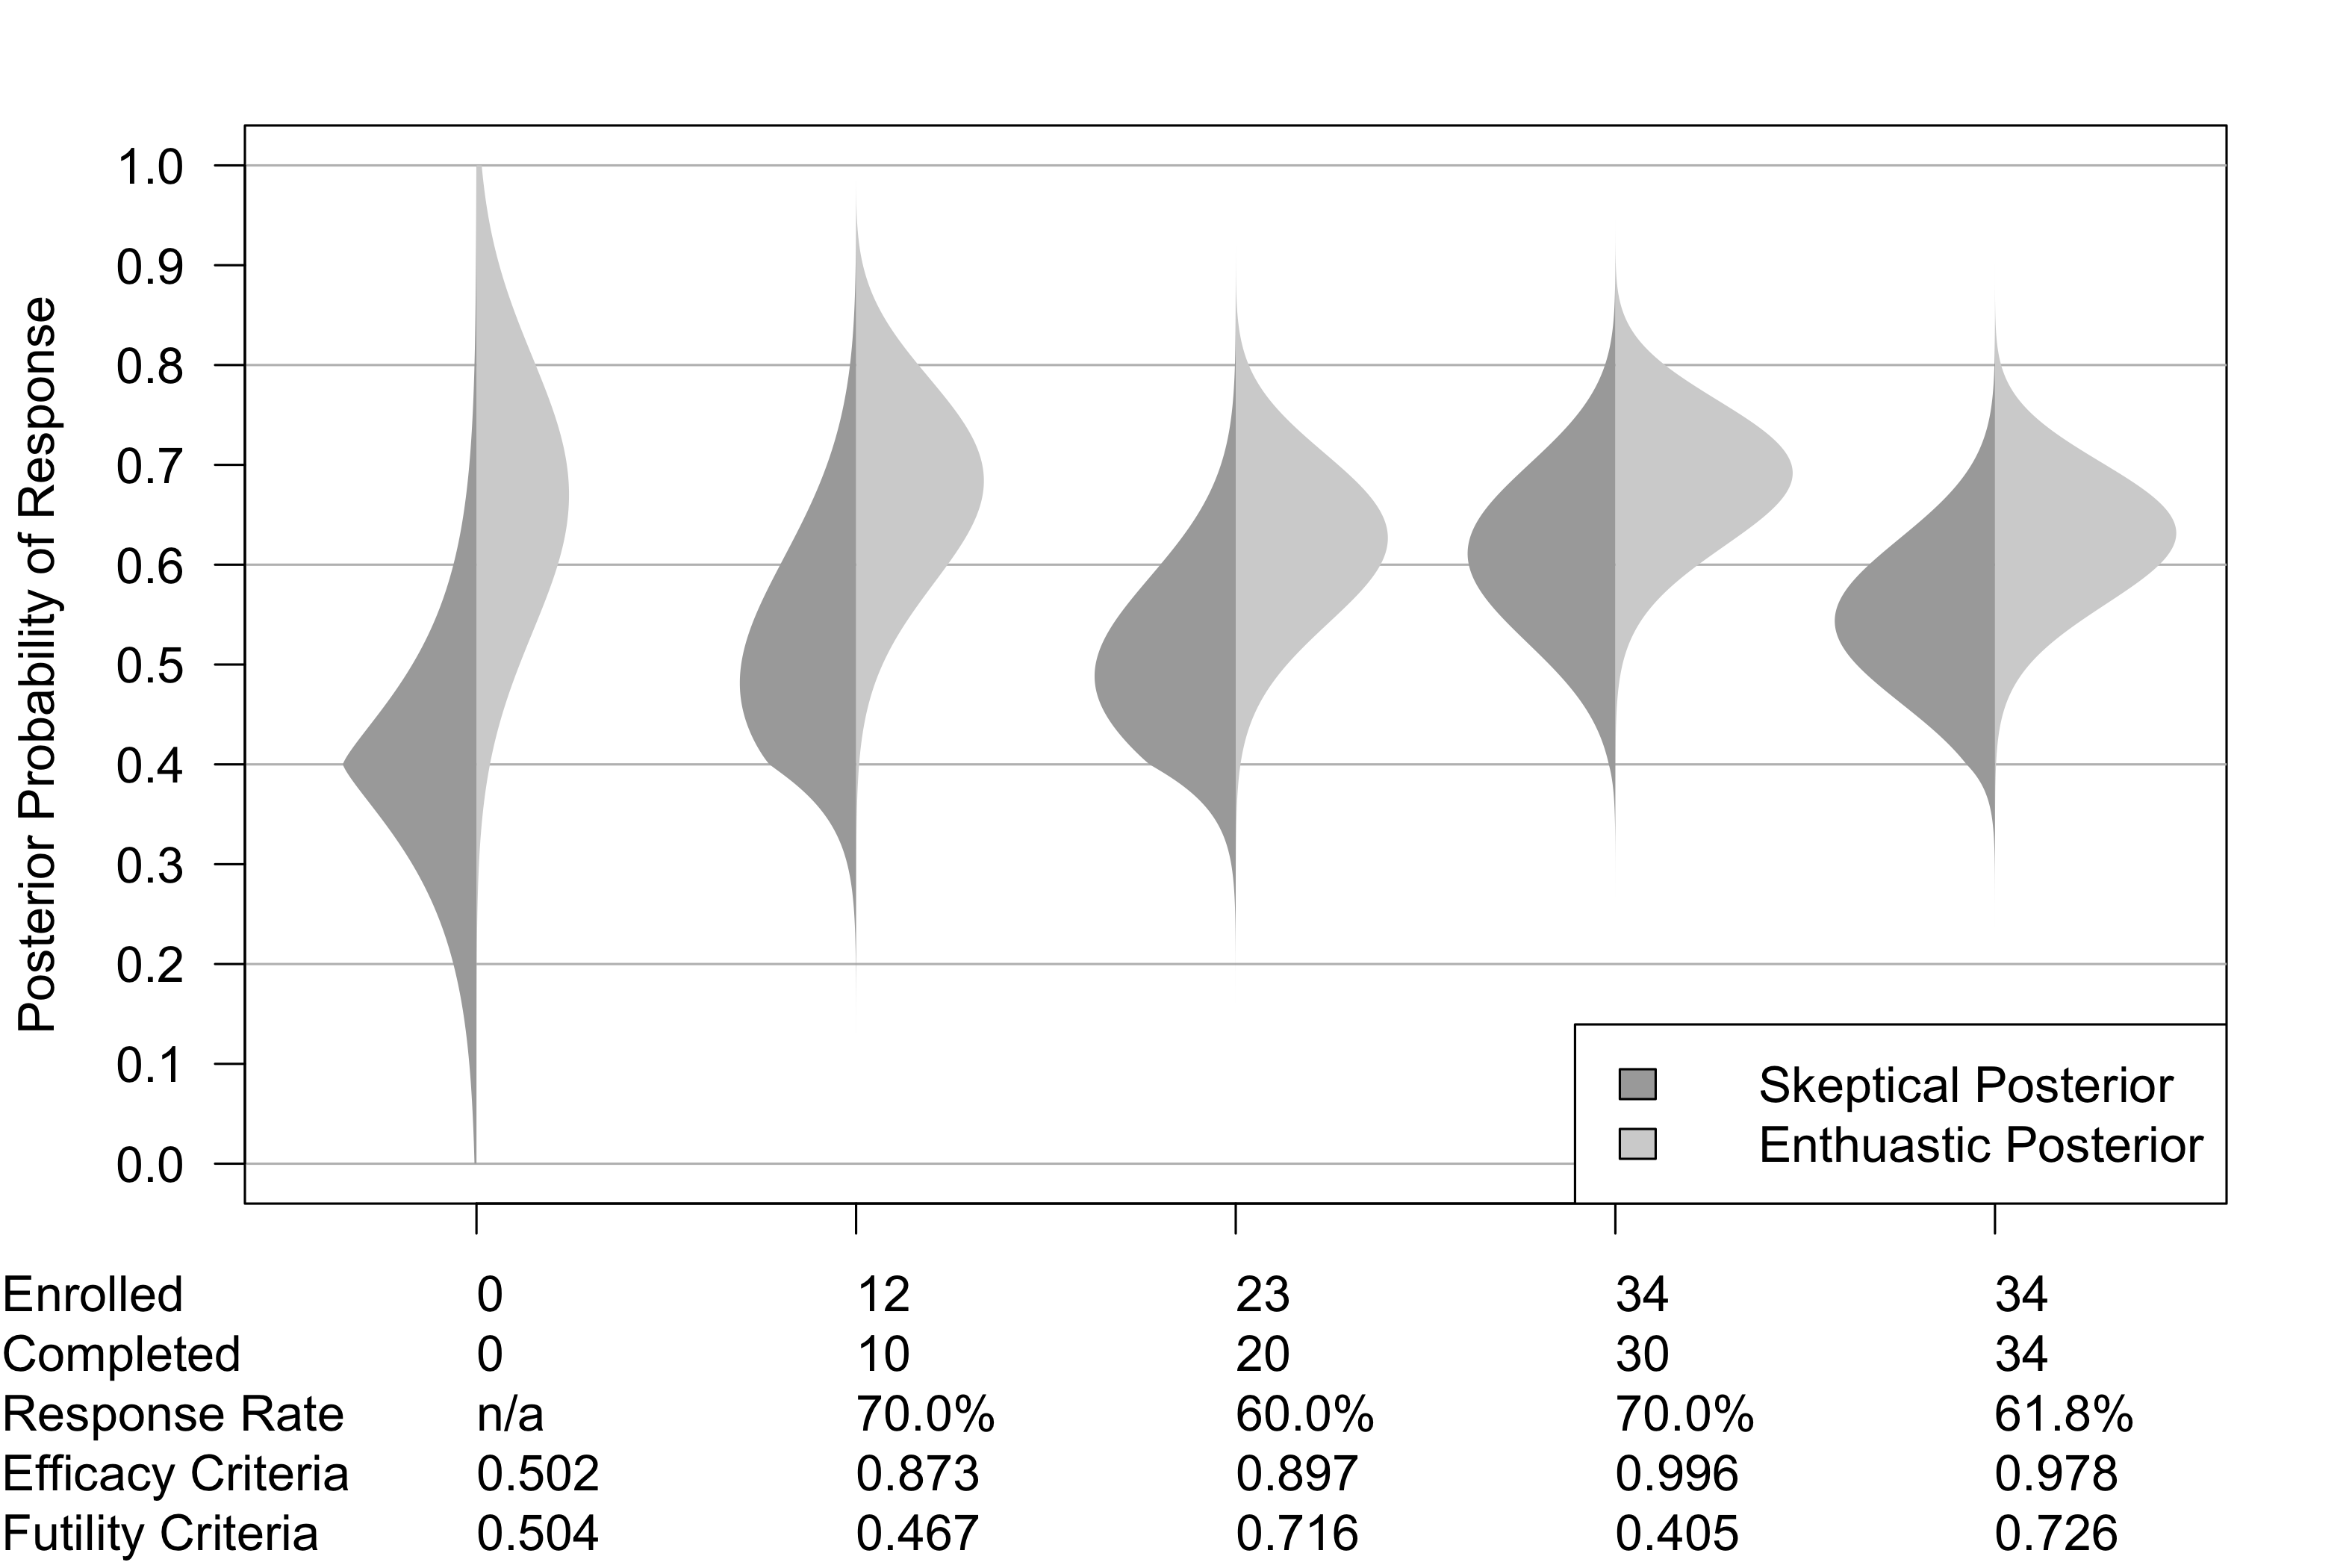
\includegraphics[width=7in]{P:/Bayesian-Sequential-Monitoring/00-paper/FIGURES/figure2a.png}
    \caption{An example path - early stopage for efficacy.}
	\label{fig:figure2a}
  \end{subfigure}
  \begin{subfigure}{7in}
    \centering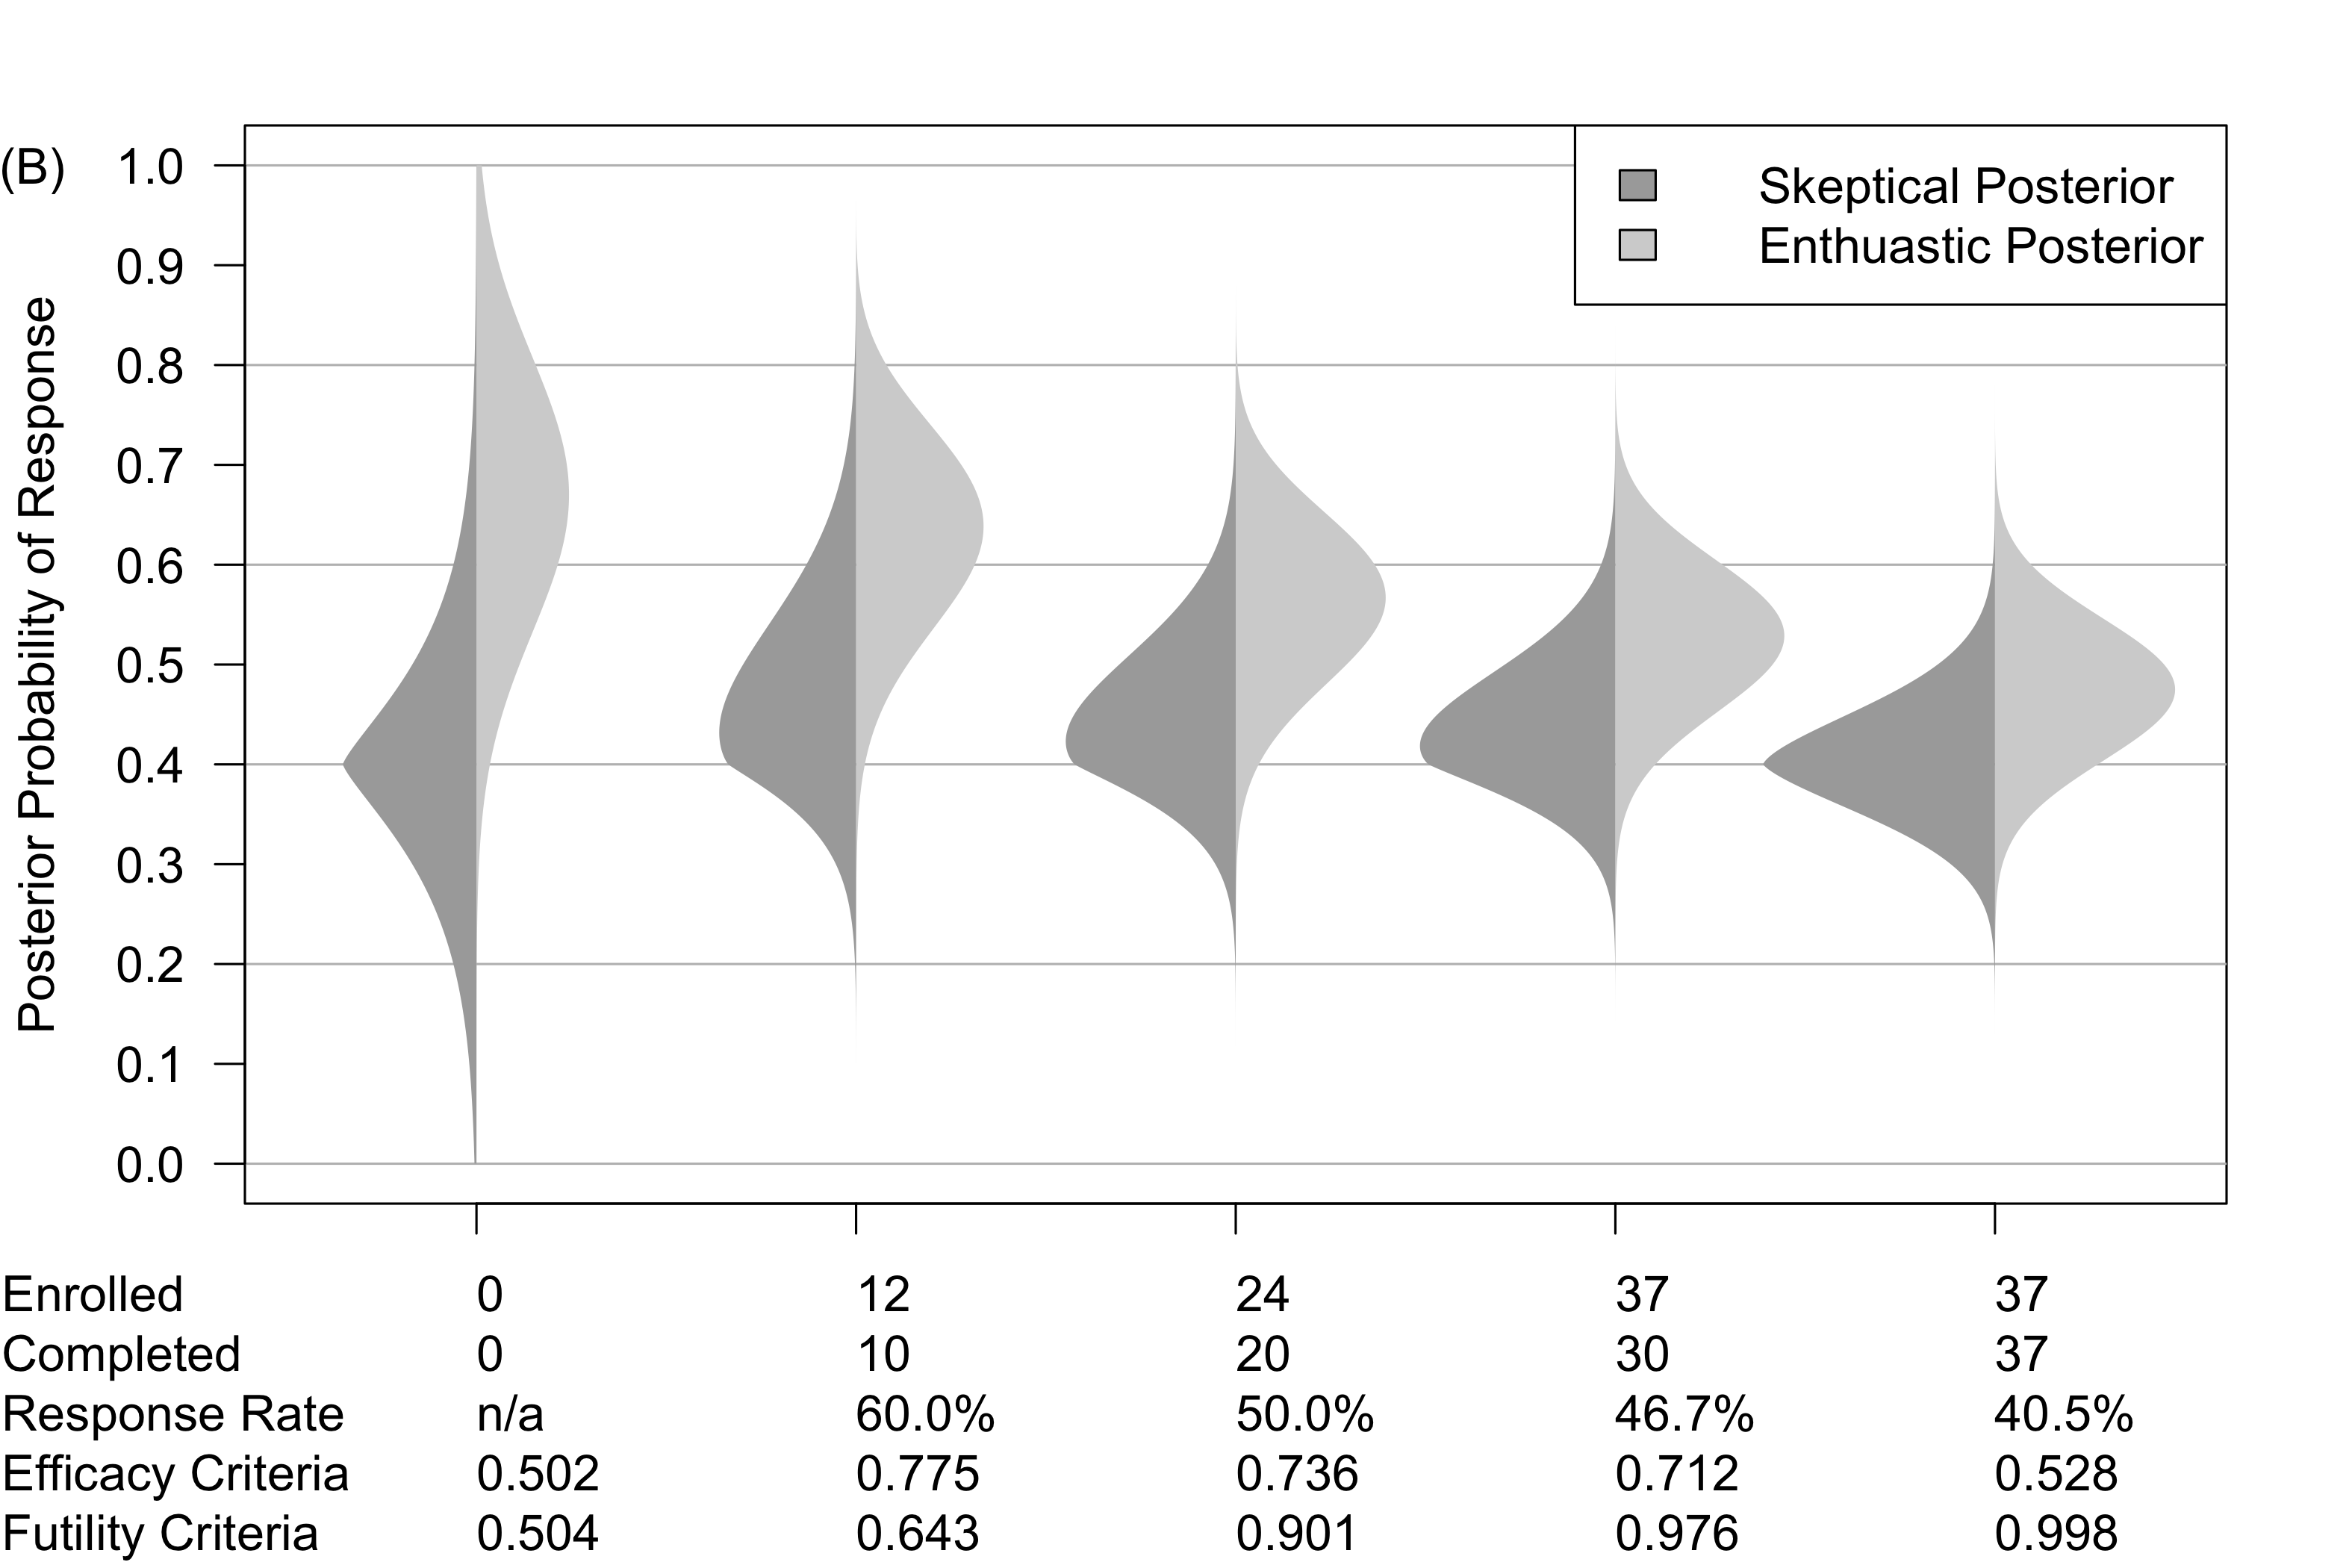
\includegraphics[width=7in]{P:/Bayesian-Sequential-Monitoring/00-paper/FIGURES/figure2b.png}
    \caption{An example path - early stoppage for futility.}
	\label{fig:figure2b}
  \end{subfigure}
 
\end{figure}
\newpage
\subsubsection{Preposterior Analysis of Operating Characteristics}
An interim analysis will be completed after every 2 subjects complete follow-up.
\begin{figure}
  \begin{subfigure}{7in}
    \centering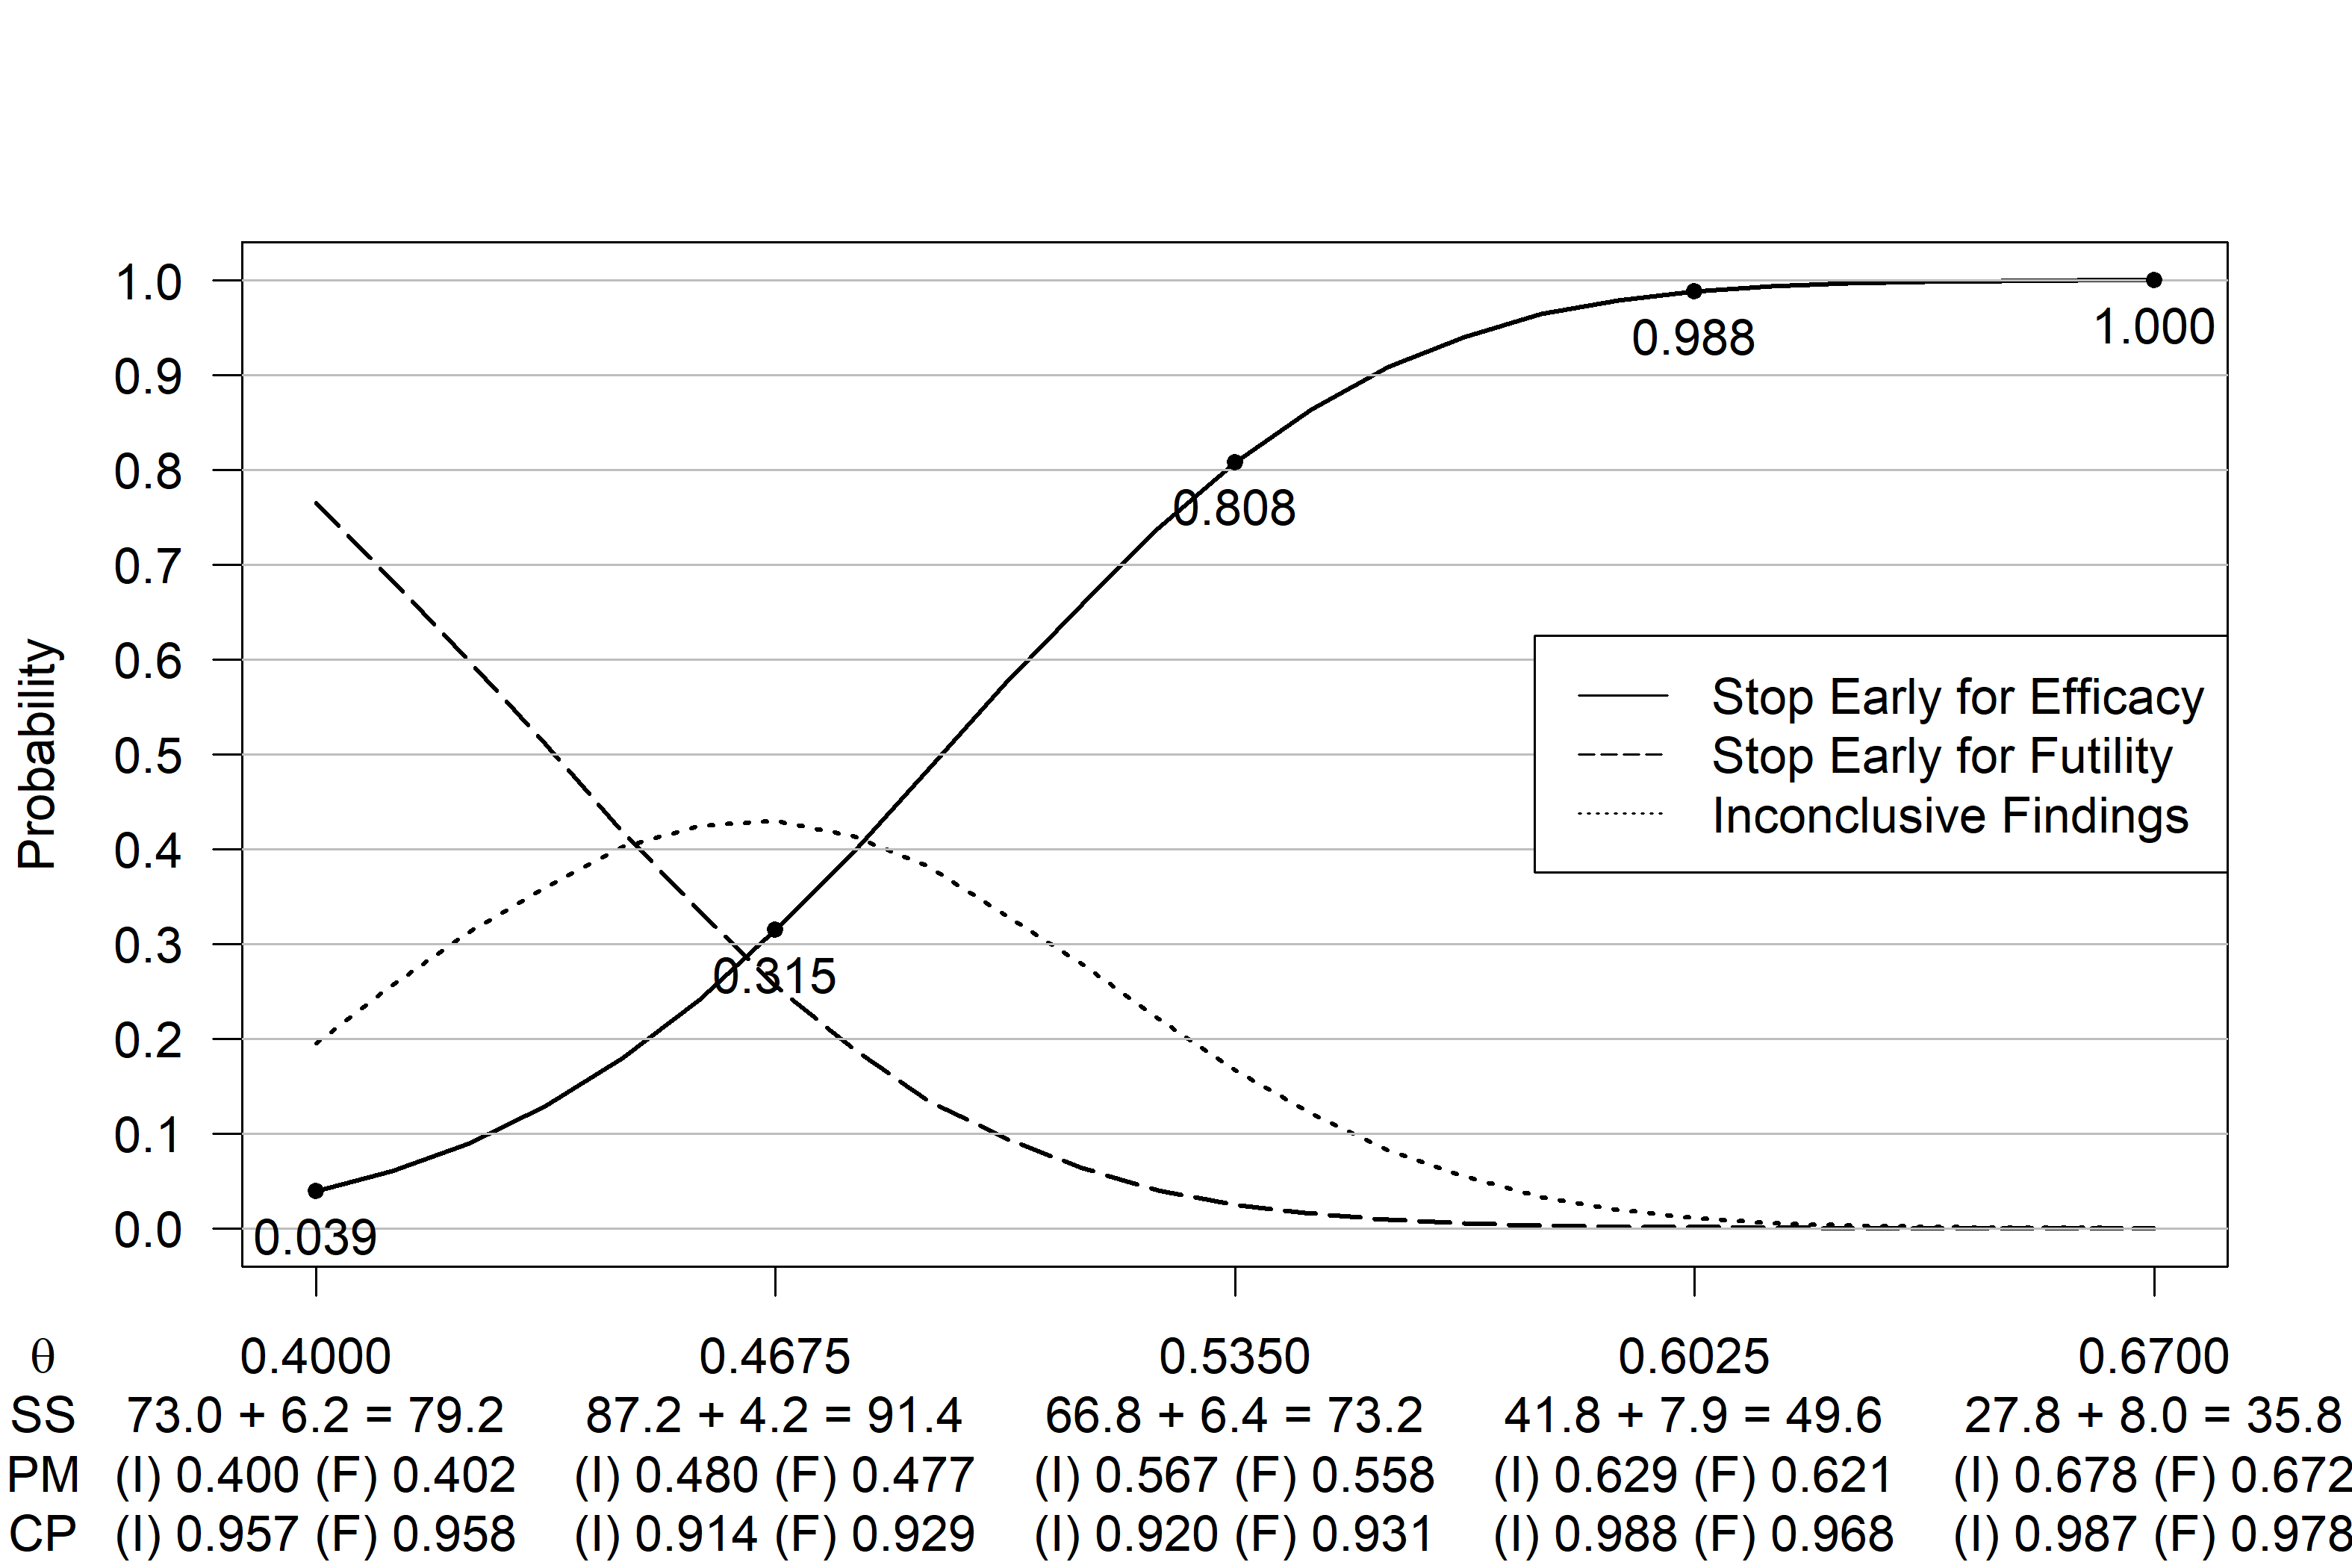
\includegraphics[width=7in]{P:/Bayesian-Sequential-Monitoring/00-paper/FIGURES/figure3a.png}
    \caption{Caption text 1}
  \end{subfigure}
  \begin{subfigure}{7in}
    \centering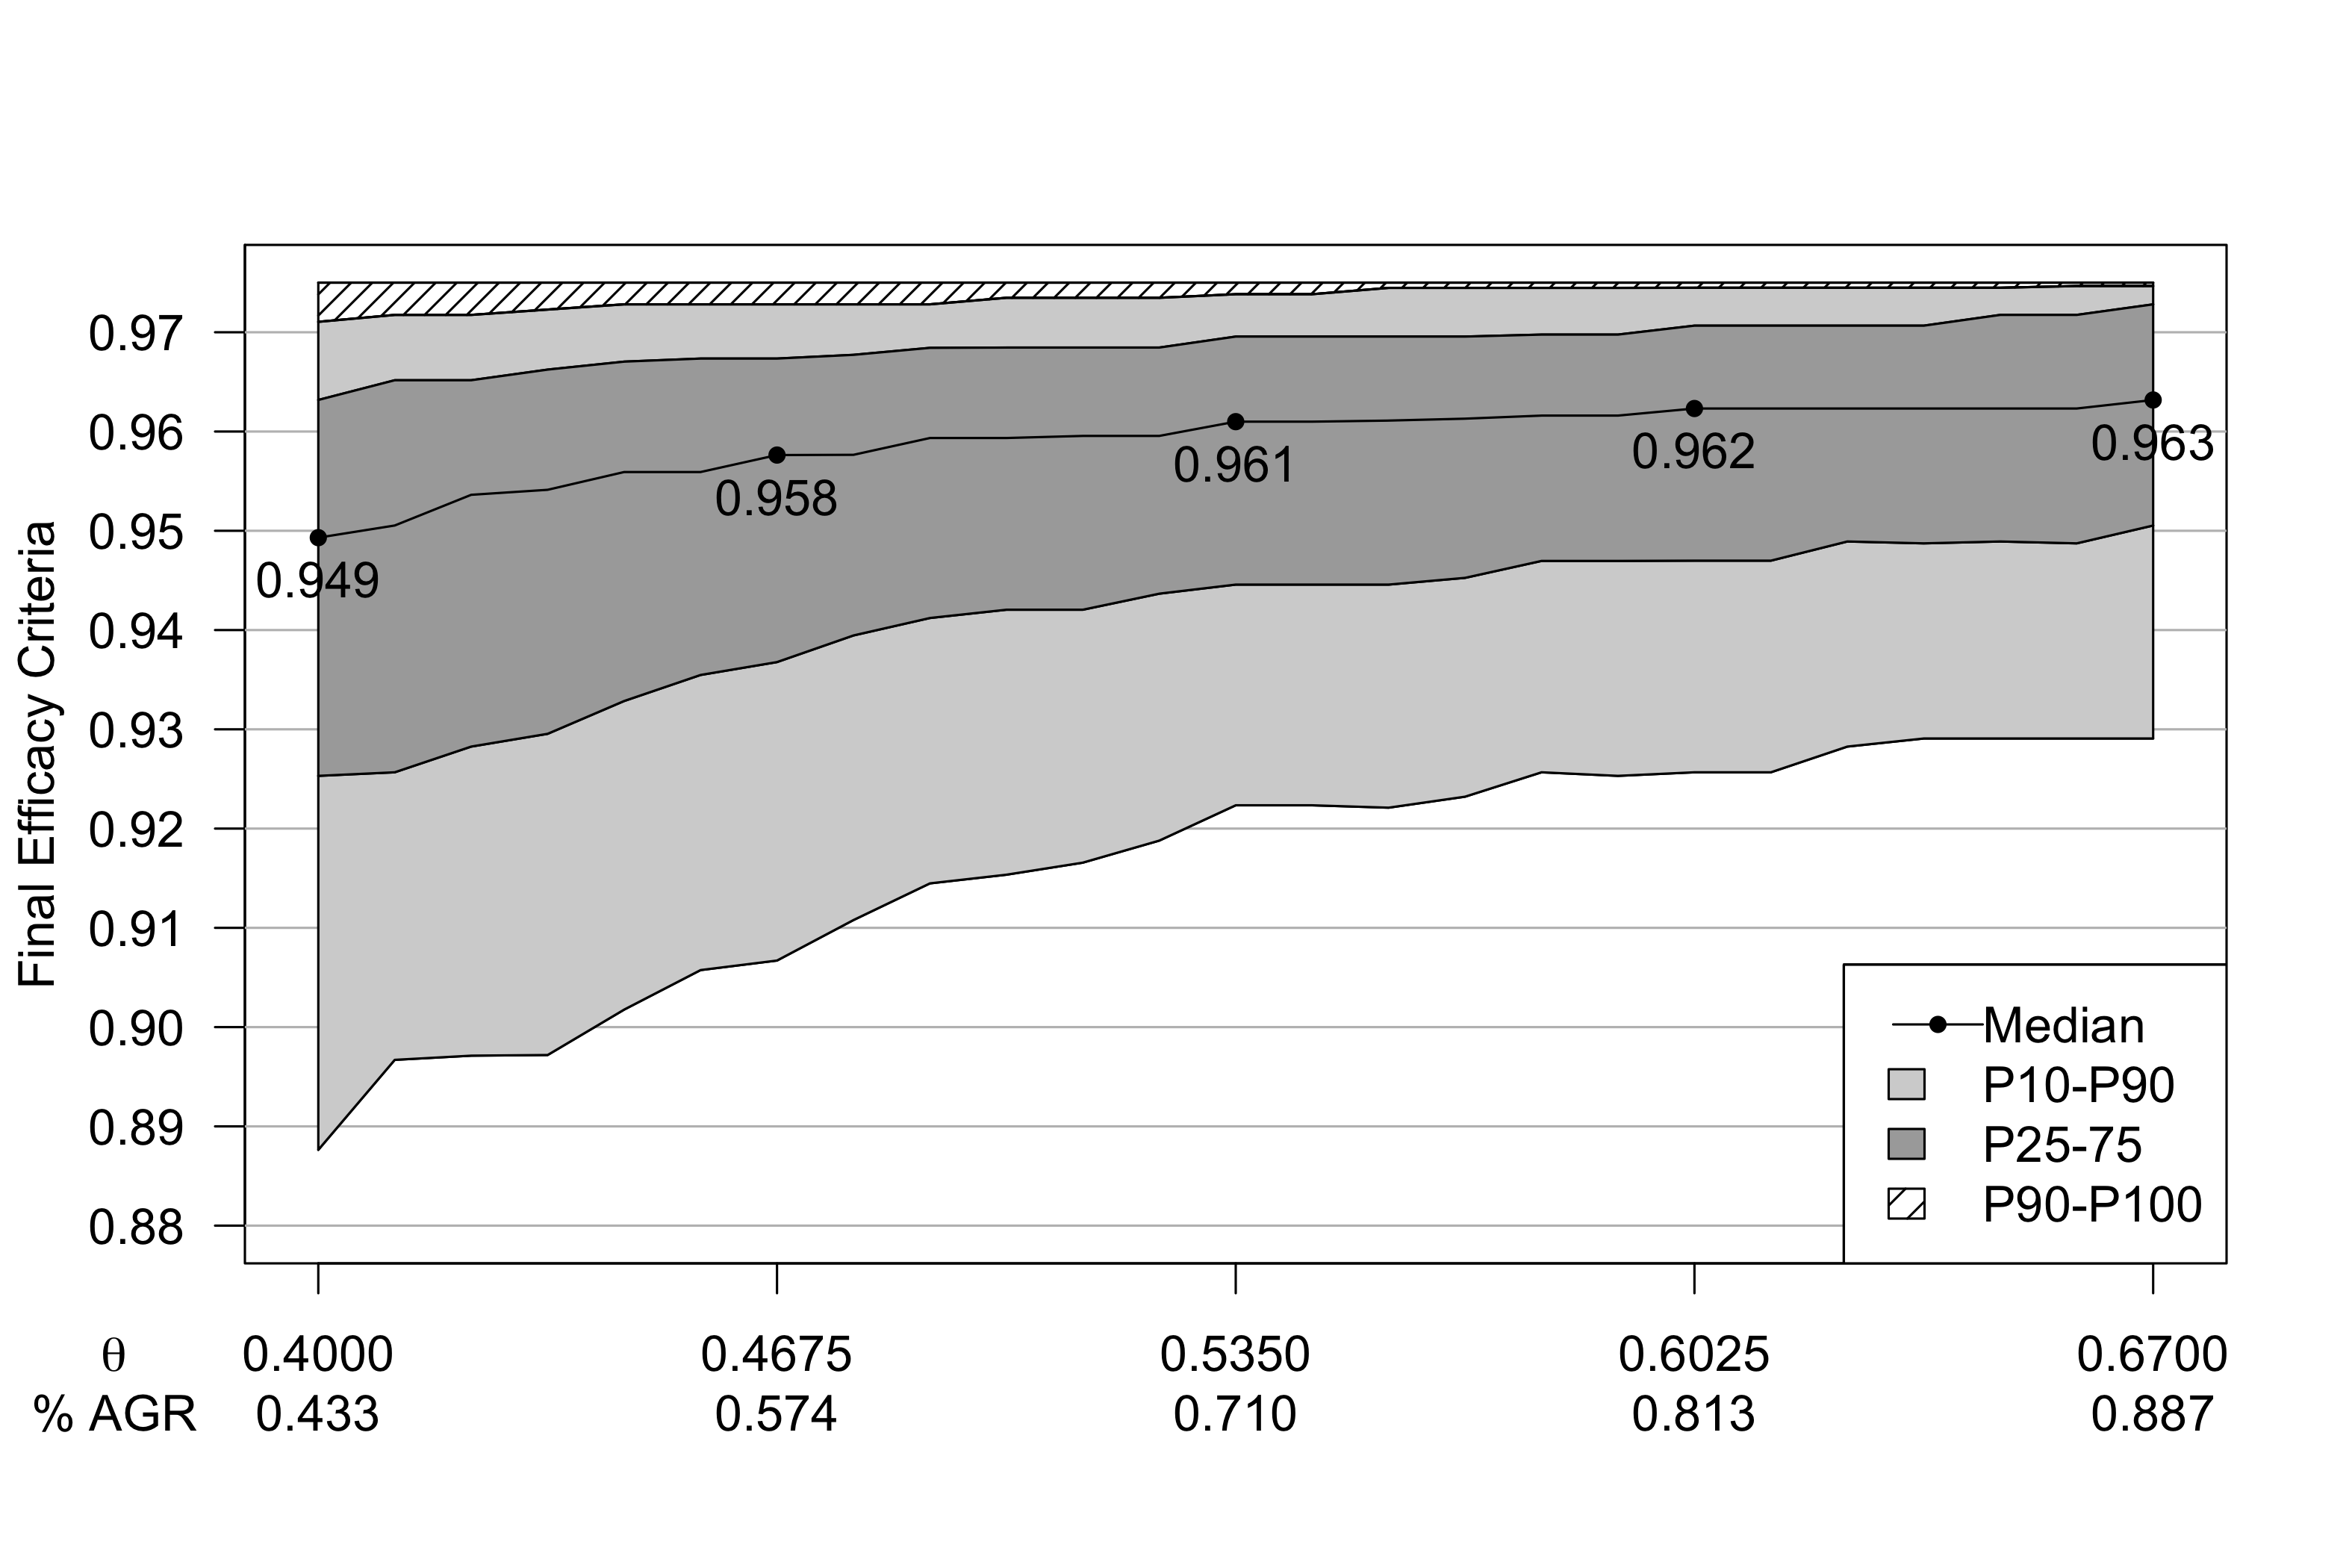
\includegraphics[width=7in]{P:/Bayesian-Sequential-Monitoring/00-paper/FIGURES/figure3b.png}
    \caption{Caption text 2}
  \end{subfigure}
 
\end{figure}

Let INC be the probability of reaching the maximum sample size without a conclusive monitoring result, let SS be the average sample size at the definitive interim analysis (I) and at the end of follow-up (F), let CP be the coverage probability using the mixture prior, and let PM be the posterior mean an inference prior which is a 50/50 mixture of the skeptical and enthusiastic priors.
%\subsubsection{Agreement between interim and final result}

%For example, at a true response rate of $\theta=0.40$, there is probability $0.894$ that the threshold for a significant result is maintained after the additional subjects complete follow-up. Conversely, with probability $0.106$ the evidence decreases, and in this case the median posterior probability is $0.93$, and a posterior probability lower than $0.88$ occurs with probability $0.1$. Thus there is a slight attenuation with respect to the dichotomous threshold, but little change in the posterior probability overall.

%\begin{figure}
%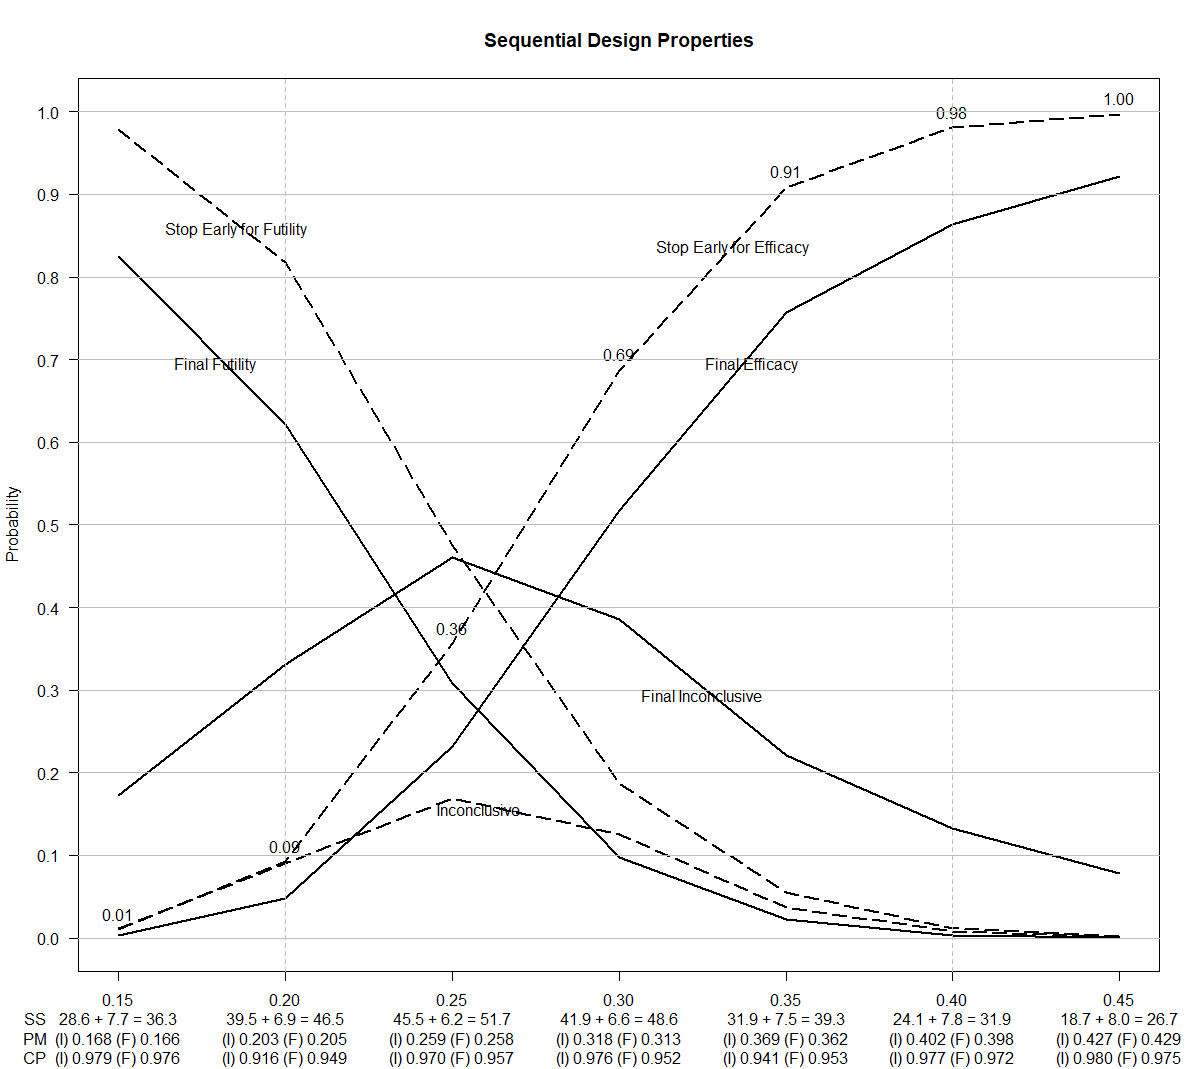
\includegraphics[width=6in]{P:/Bayesian-Sequential-Monitoring/00-paper/FIGURES/sequential_design_properties_2}
%\caption{Shows agreement between sequential and final determinations as they relate to the strict cut-offs}
%\end{figure}

%\subsubsection*{Vemurafenib Trial }
%``In this study, a response rate of 15\% at week
%8 was considered to be low, a response rate of
%45\% was considered to be high, and a response
%rate of 35\% was considered to be low but still
%desirable and indicative of efficacy. Assuming
%response rates as specified in the hypothesis testing, a power of 80\% for a high response rate and
%70\% for the low but still desirable response rate,
%and a two-sided alpha level of 0.1, we calculated
%that the number of patients required in each
%cohort would be 7, 13, or 19, depending on the
%results obtained."

\subsubsection{Type 1 error rate by the frequency of data monitoring}
As expected, the probability of stopping enrollment due to a promising interim trial result and the Type 1 error rate at the final analysis increase with the frequency of interim monitoring, however, the increase is very slight at the final analysis. Regardless of frequency of monitoring there are good Type 1 error rates. 

%Even at the extreme case where an interim analysis is conducted after every outcome, the probability of stopping at the interim due to a promising result when the true response is at the null level is only $0.108$ (about double the nominal rate), and even in this situation the Type 1 error rate once follow-up is complete does not exceed $0.05$. Thus Bayesian sequential monitoring has good frequentist properties even with frequent interim analyses.
%\begin{itemize}
%\item The two sides of the discussion: first is what happens during the trial regarding sequential monitoring, such as \% of time stopping early vs. trial done to completion and expected sample size. Second is the final determination of efficacy or futility and how that relates to Type 1 Error and power. 
%\item  Remember the best case for sequential monitoring is slow enrollment relative to outcome ascertainment. Slow enrollment means there is a benefit to ending trial early and reach a conclusion faster. Outcome ascertainment needs to be somewhat fast to ensure a good \# of outcomes are generated.
%\end{itemize}
%\begin{itemize}
%\item Want to highlight that the ultimate inference will have no Type 1 error inflation. At this point the ultimate inference for efficacy is still made with skeptical prior.
%\item Label lines nicely.
%\item ``Only bad thing to do is to stop learning"
%\item Enrollment rate and \% of ongoing data as operating characteristics are interesting ideas, but focus on the plots already created.
%\item Mat: Scaling on \# of subjects in each interim analysis rather than \# of interim analyses (e.g. flip X axis). Make labels go vertical or diagonal.
%\end{itemize}
\begin{figure}
  \begin{subfigure}{7in}
    \centering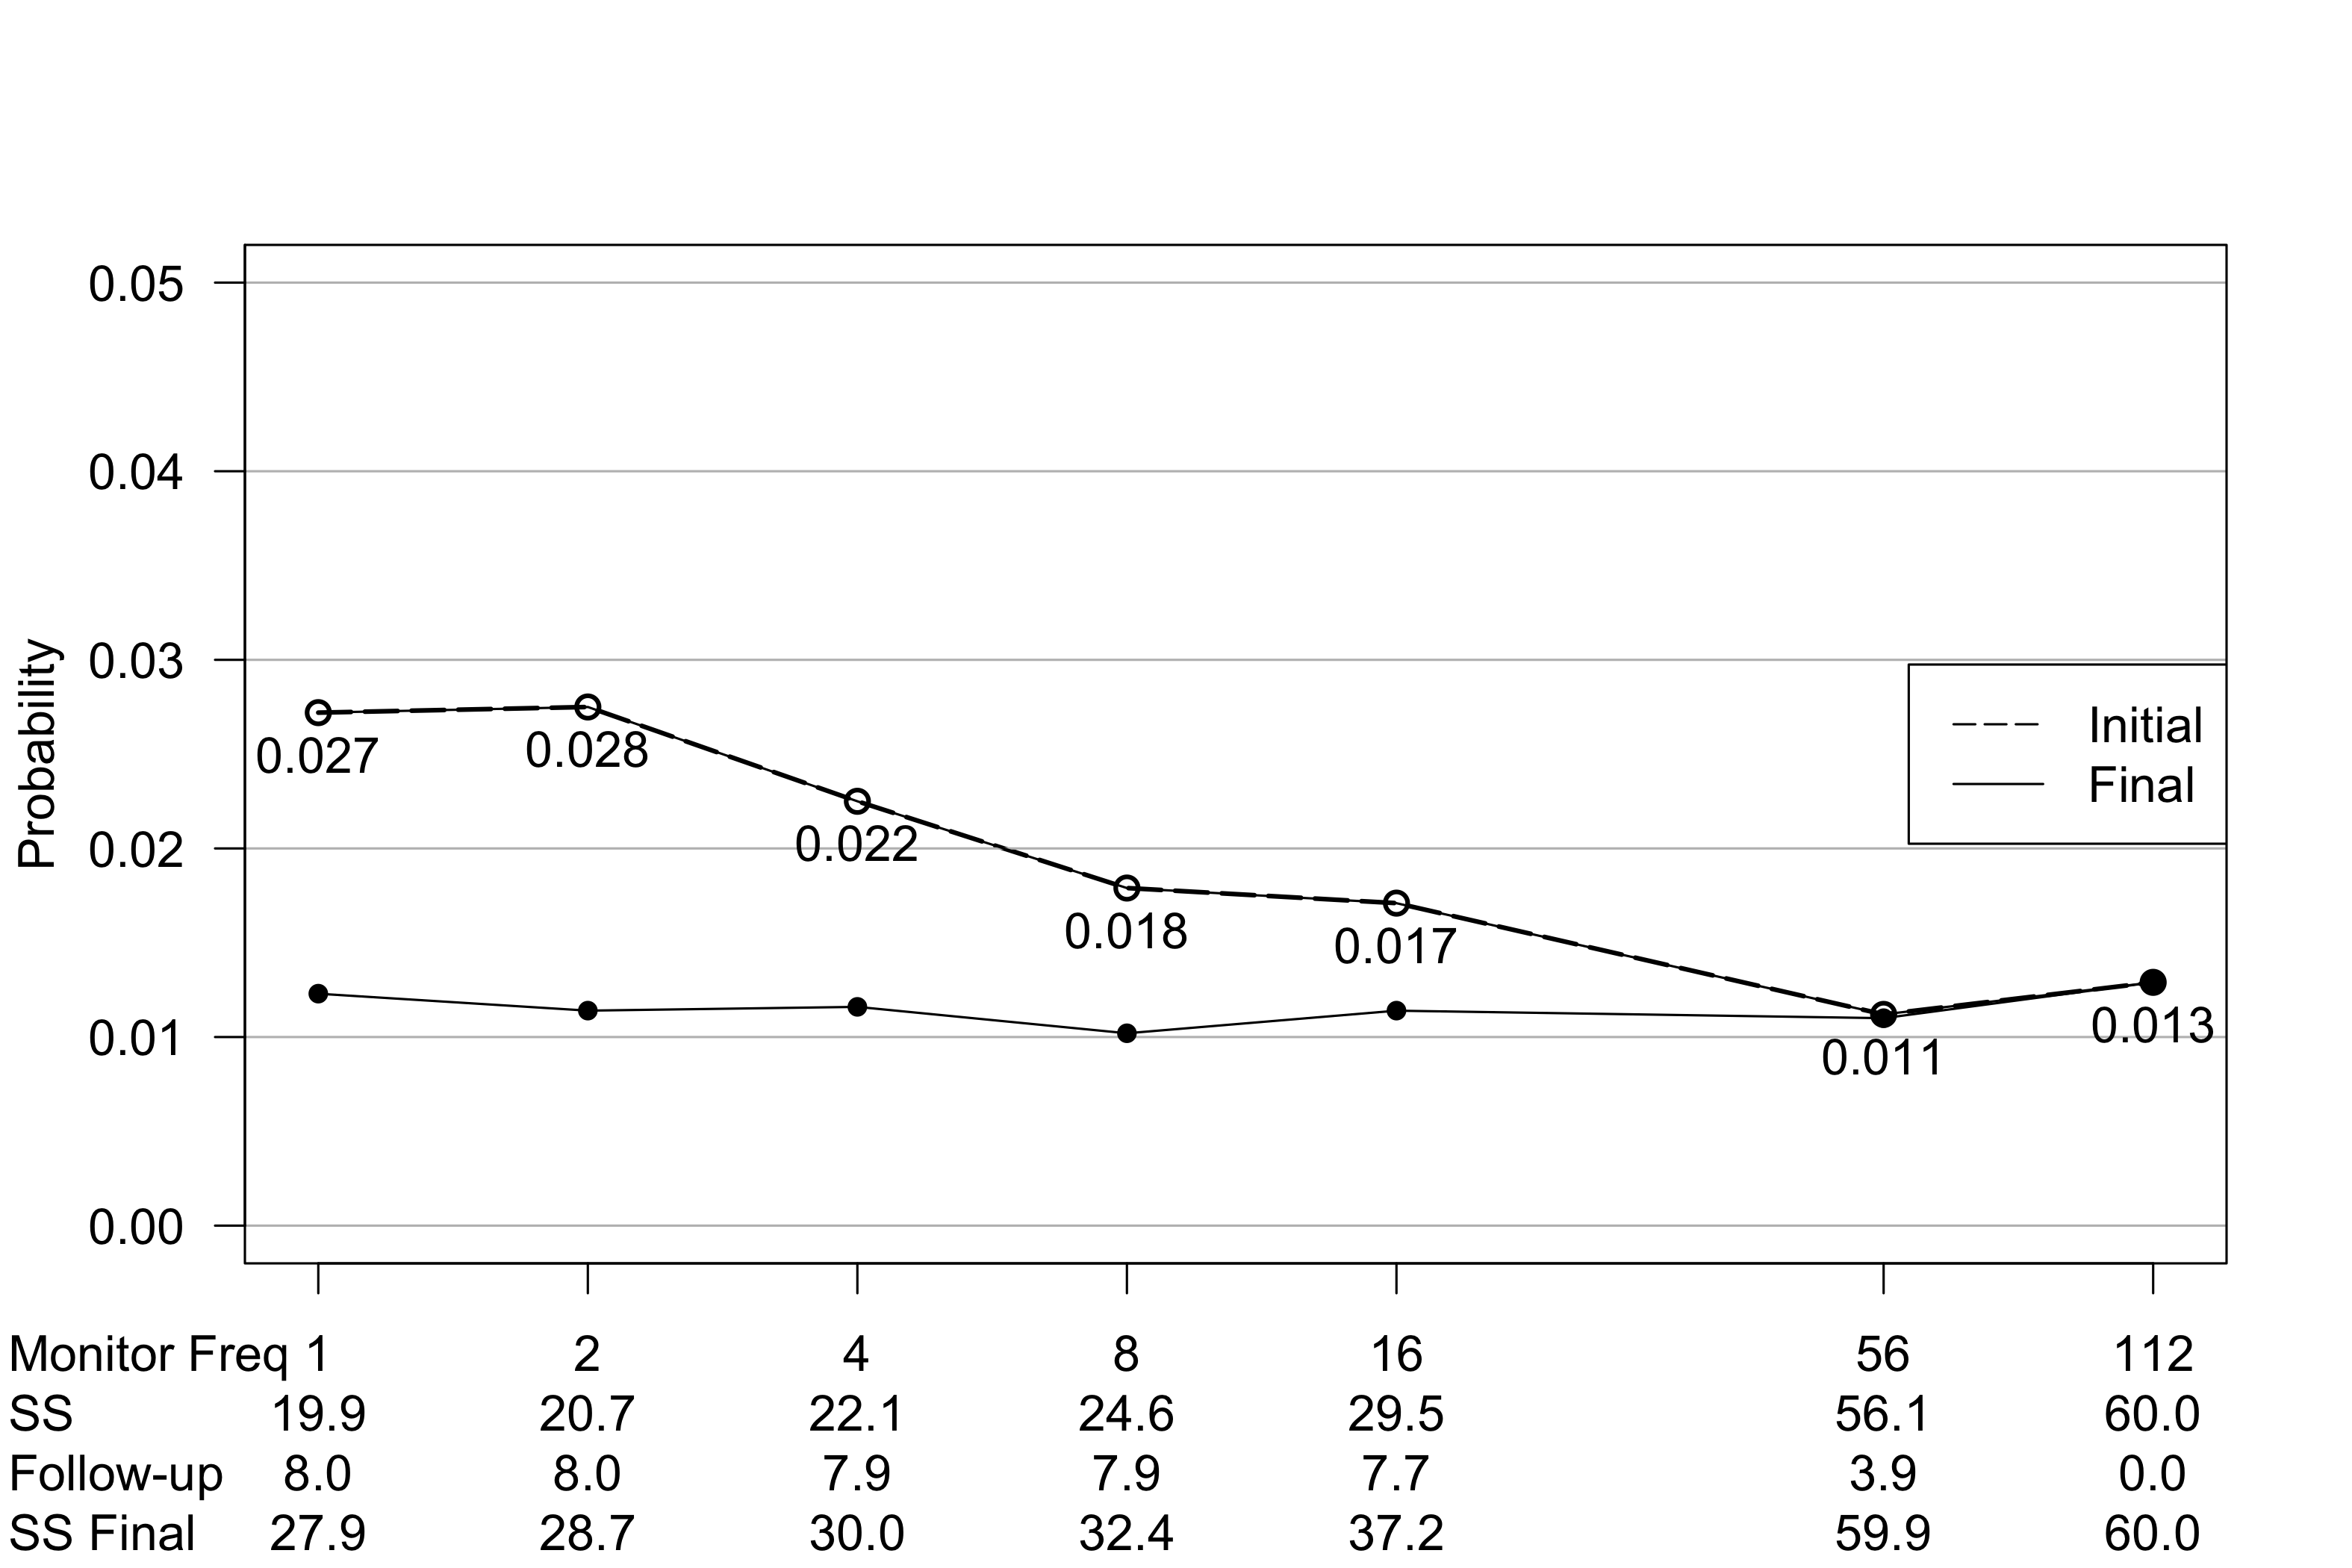
\includegraphics[width=7in]{P:/Bayesian-Sequential-Monitoring/00-paper/FIGURES/figure4.png}
    \caption{Caption text 1}
  \end{subfigure}
  \begin{subfigure}{7in}
    \centering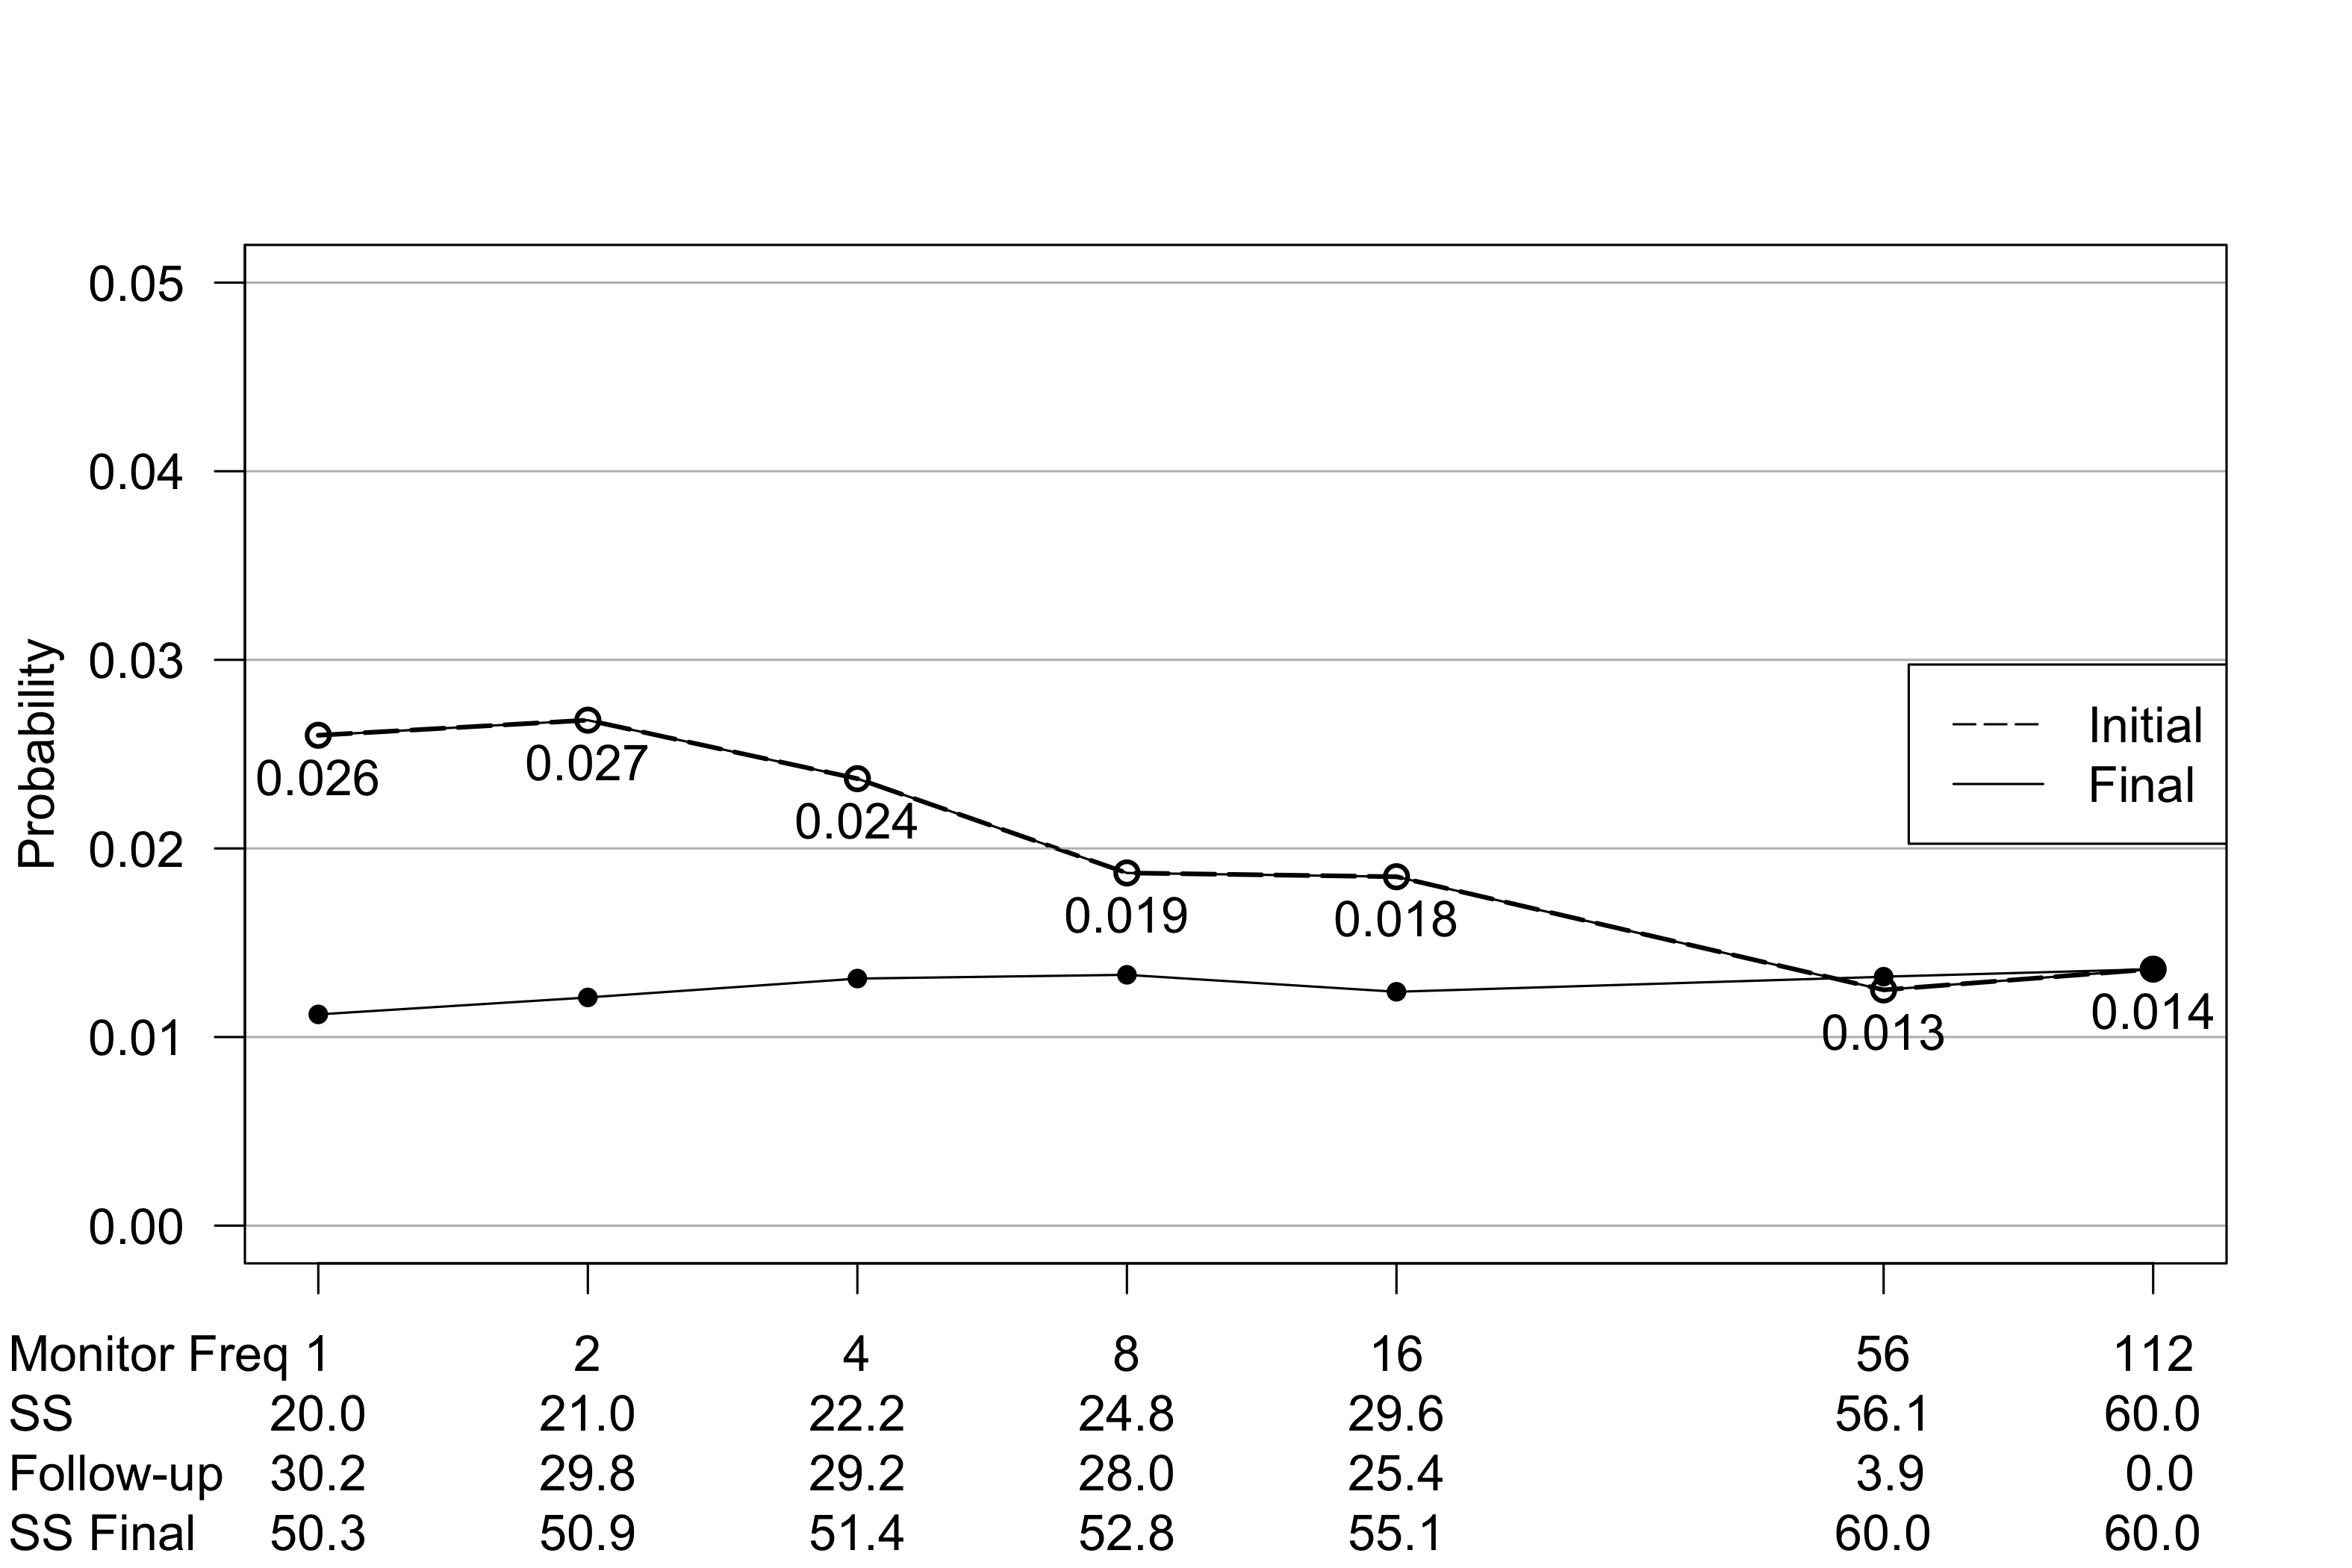
\includegraphics[width=7in]{P:/Bayesian-Sequential-Monitoring/00-paper/FIGURES/figureS1.png}
    \caption{Caption text 2}
  \end{subfigure}
 
\end{figure}

Monitoring Freq \textcolor{green}{never abbreviate words} is 1 for fully sequential design and 112 when the only analysis is with all completed outcomes.
\subsection{Parallel Two-Group Design with Binary Endpoint}
\subsubsection{Motivating example}
The Pediatric Lupus Trial of Belimumab Plus Background Standard Therapy (PLUTO) trial, was a multi-center study to evaluate the safety, pharmacokinetics, and efficacy of belimumab intravenous (IV) in pediatric patients 5 to 17 years of age with active systemic lupus erythematosus. 

The goal was to test for superiority of belimumab to placebo. Based on adult studies, a response rate of $0.51$ was expected for belimumab and based on previous research a response rate of $0.39$ was expected for placebo.

The study design included enrollment of 100 subjects, the first 24 subjects randomized in a 5:1 ratio (belimumab:placebo) and the remaining 76 subjects would be randomized in a 1:1 allocation ratio. Therefore, 58 subjects would be randomized to belimumab and 42 to placebo. The sample size was based on feasibility constraints rather than a power calculation.

The binary response endpoint was evaluated at 52 weeks post enrollment. The study start date was September 7, 2012, and the primary completion date was January 24, 2018. Since the follow-up period is 52 weeks the last enrollment is estimated to be a year prior to the primary competition date yielding an average enrollment rate of one enrollment per $17.2$ days.
\subsubsection{Model formulation}
Let $\theta_0$ represent the response rate the control group and $\theta_1$ represent the response probability for the investigational product (IP) group. 
Consider the hypothesis testing of IP superiority to control
\begin{align*}
H_0:\theta_1-\theta_0\leq 0\text{ vs. }H_1: \theta_1-\theta_0>0.
\end{align*}

The priors will be chosen based on the joint specification in (\ref{eq:generalized_normal_joint}). First, a prior on the response probability for the placebo group is given in the form of (\ref{eq:generalized_normal_PC}). This prior is chosen to be flat in the region $0.39\pm 0.10$.

To complete the joint specification of (\ref{eq:generalized_normal_joint}), skeptical and enthusiastic priors of the form (\ref{eq:generalized_normal_IP}) will be parameterized as to satisfy (\ref{eq:enthprior}) and (\ref{eq:skptprior}). The skeptic believes there is no difference in response rates by treatment group, and the enthusiastic person believes the IP group will have a response rate probability that is 0.12 higher than the placebo group. 

%This corresponds to $\delta_S=0$ and $\delta_E=0.12$. The skeptical and enthusiastic priors are defined as
%\begin{align*}
%\pi_S(\theta_0,\theta_1)=&\exp\left\{-\frac{1}{2}\left(\frac{\theta_0-\mu}{\sigma_S}\right)^{2}\right\}\times \exp\left\{-\frac{1}{2}\left(\frac{(\theta_1-\theta_0)-\delta_S}{\sigma_{S1}}\right)^{2}\right\}\times I((\theta_0,\theta_1)\in [0,1]\times[0,1]) /c_S,\\
%\pi_E(\theta_0,\theta_1)=&\exp\left\{-\frac{1}{2}\left(\frac{\theta_0-\mu}{\sigma_E}\right)^{2}\right\}\times \exp\left\{-\frac{1}{2}\left(\frac{(\theta_1-\theta_0)-\delta_E}{\sigma_{E1}}\right)^{2}\right\}\times I((\theta_0,\theta_1)\in [0,1]\times[0,1]) /c_E
%\end{align*}
%
%where $c_S$ and $c_E$ are normalizing constants. The values of $\sigma_S$ and $\sigma_{S1}$ are chosen such that $P(\theta_1-\theta_0>0.1|\pi_S)=0.05$. Similarly, $\sigma_E$ and $\sigma_{E1}$ are chosen such that $P(\theta_1-\theta_0\leq0|\pi_E)=0.05$.

%\begin{align*}
%\pi(\theta_0,\theta_1)\propto& \hspace{0.05in}exp \left\{-\frac{1}{2}\left|\frac{(\theta_1-\theta_0)-\delta}{\sigma}\right|^\alpha\right\}
%\end{align*}


%Here we wish to elicit pessimistic and enthusiastic priors consistent with the following:
% \begin{enumerate}
%  \item The control group response probability is expected to be approximately $0.20$ and investigators are relatively sure
%		    that the it will be between 0.5 and 0.35.
%				
%	\item The IP group response probability is likely to provide an improvement of approximately 0.20.
%\end{enumerate}

Enrollment will proceed until one of the following three conditions are satisfied:
\begin{align*}
\text{Efficacy criteria (EFF): }&P(\theta_1-\theta_0>0|\mathbf{D},\pi_S)\geq 0.975\\
\text{Futility criteria (FUT): }&P(\theta_1-\theta_0 \leq 0.06|\mathbf{D},\pi_E)\geq 0.975\\
\text{Maximum sample size: }&N=100 \text{ patient outcomes}
\end{align*}

An interim analysis is competed after every 10 subjects have completed outcomes.

\subsubsection{Design properties: Results}

Simulations were run fixing the placebo response rate at $\theta_0=0.39$ and varying the treatment response rate $\theta_1\in[0.39,0.51]$. Due to the low maximum sample size, no simulations resulted in the efficacy criteria $(P(\theta_1-\theta_0>0|\mathbf{D},\pi_S)\geq 0.975)$ being satisfied. Instead of the skeptical prior $\pi_S$ being used for the efficacy criteria, an inference prior $\pi_I$ of the form (\ref{eq:inference_prior}) is used where the choice of $\omega$ in (\ref{eq:omega_formula}) is determined based on varying $p(\pi_S)$ and $p(\pi_E)$ at the outset.

\begin{figure}
    \centering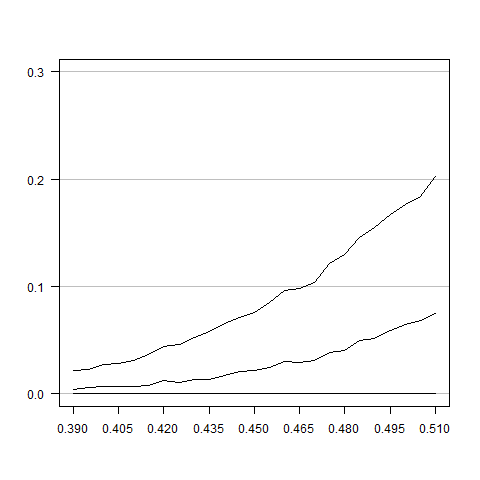
\includegraphics[width=3.5in]{P:/Bayesian-Sequential-Monitoring/00-paper/FIGURES/figure6.png}
    \caption{Caption text 2}
 \end{figure}


\section{Discussion}

Text.
\section{Supplementary material}
\subsection{Shape parameter specification}\label{sec:shapeParameterSpecification}
\subsection{Risk difference prior parameterization}\label{sec:riskDiffPriorParm}
\subsubsection{Type 1 error rate depending on enrollment schemes}

\newpage
\subsubsection{Robustness of parameterizations of monitoring priors}
\begin{figure}
  \begin{subfigure}{7in}
    \centering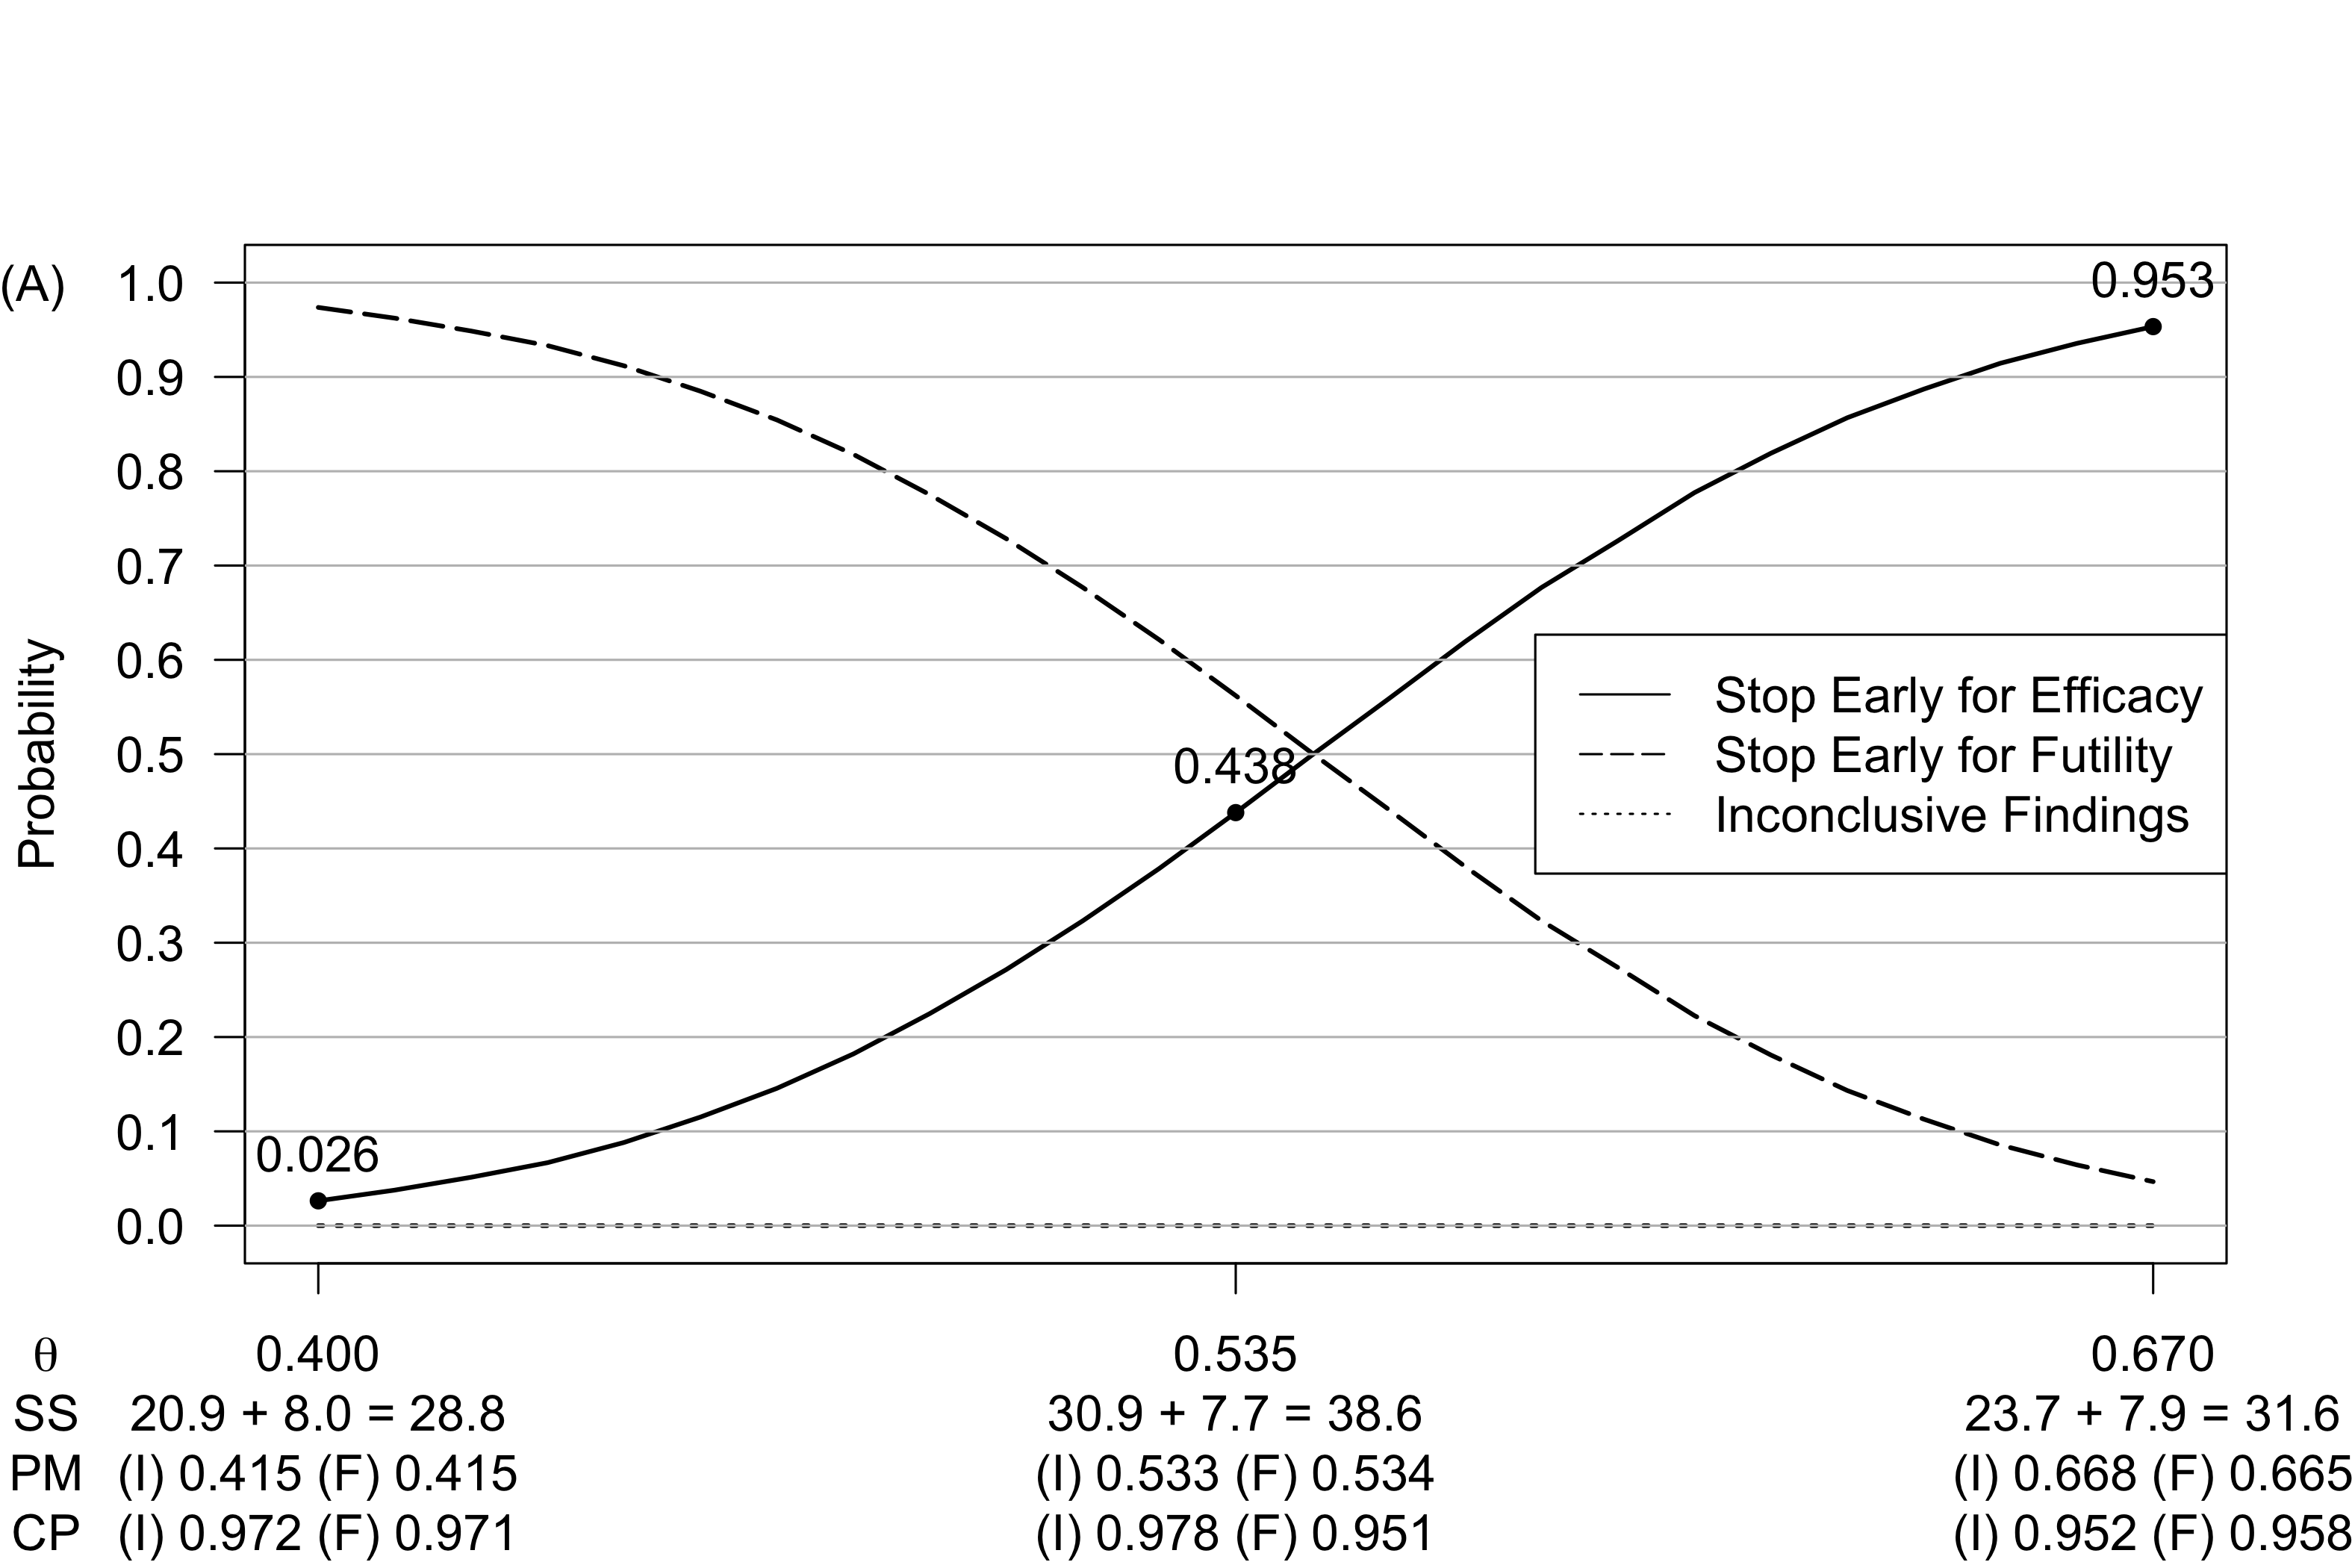
\includegraphics[width=7in]{P:/Bayesian-Sequential-Monitoring/00-paper/FIGURES/figureS2a.png}
    \caption{Caption text 1}
  \end{subfigure}
  \begin{subfigure}{7in}
    \centering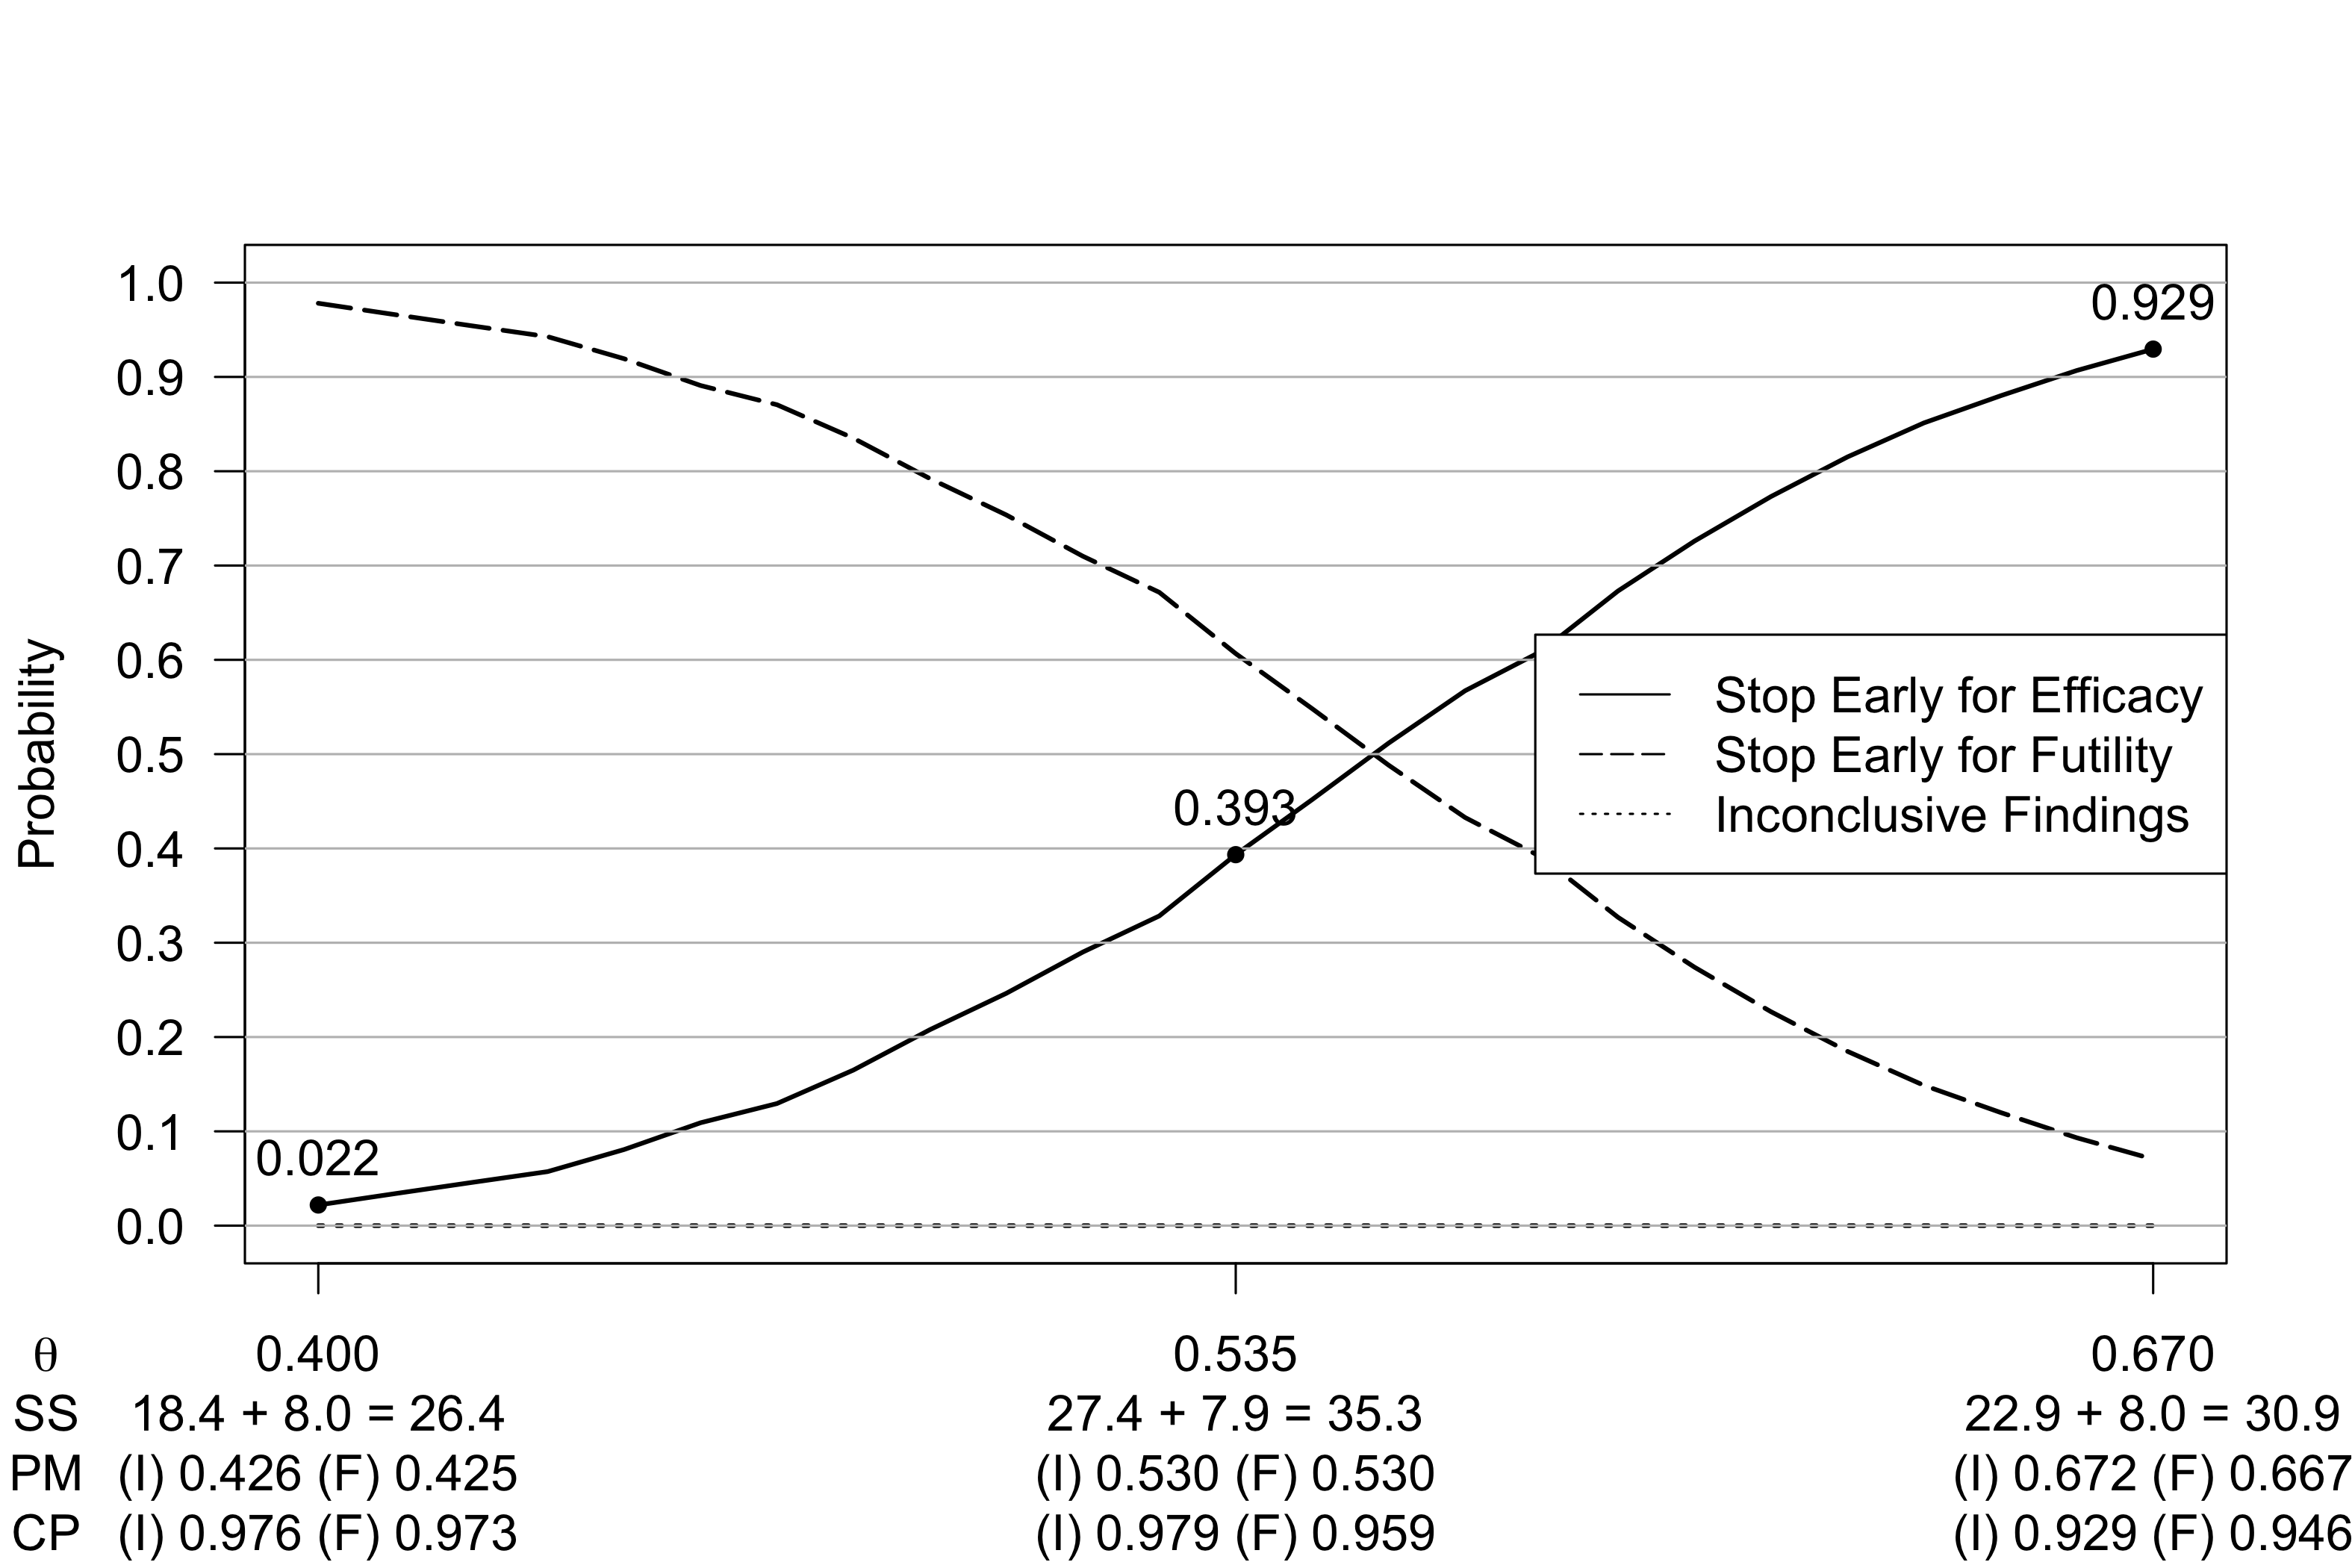
\includegraphics[width=7in]{P:/Bayesian-Sequential-Monitoring/00-paper/FIGURES/figureS2b.png}
    \caption{Caption text 2}
  \end{subfigure}
 \end{figure}
\begin{figure}
  \begin{subfigure}{7in}
    \centering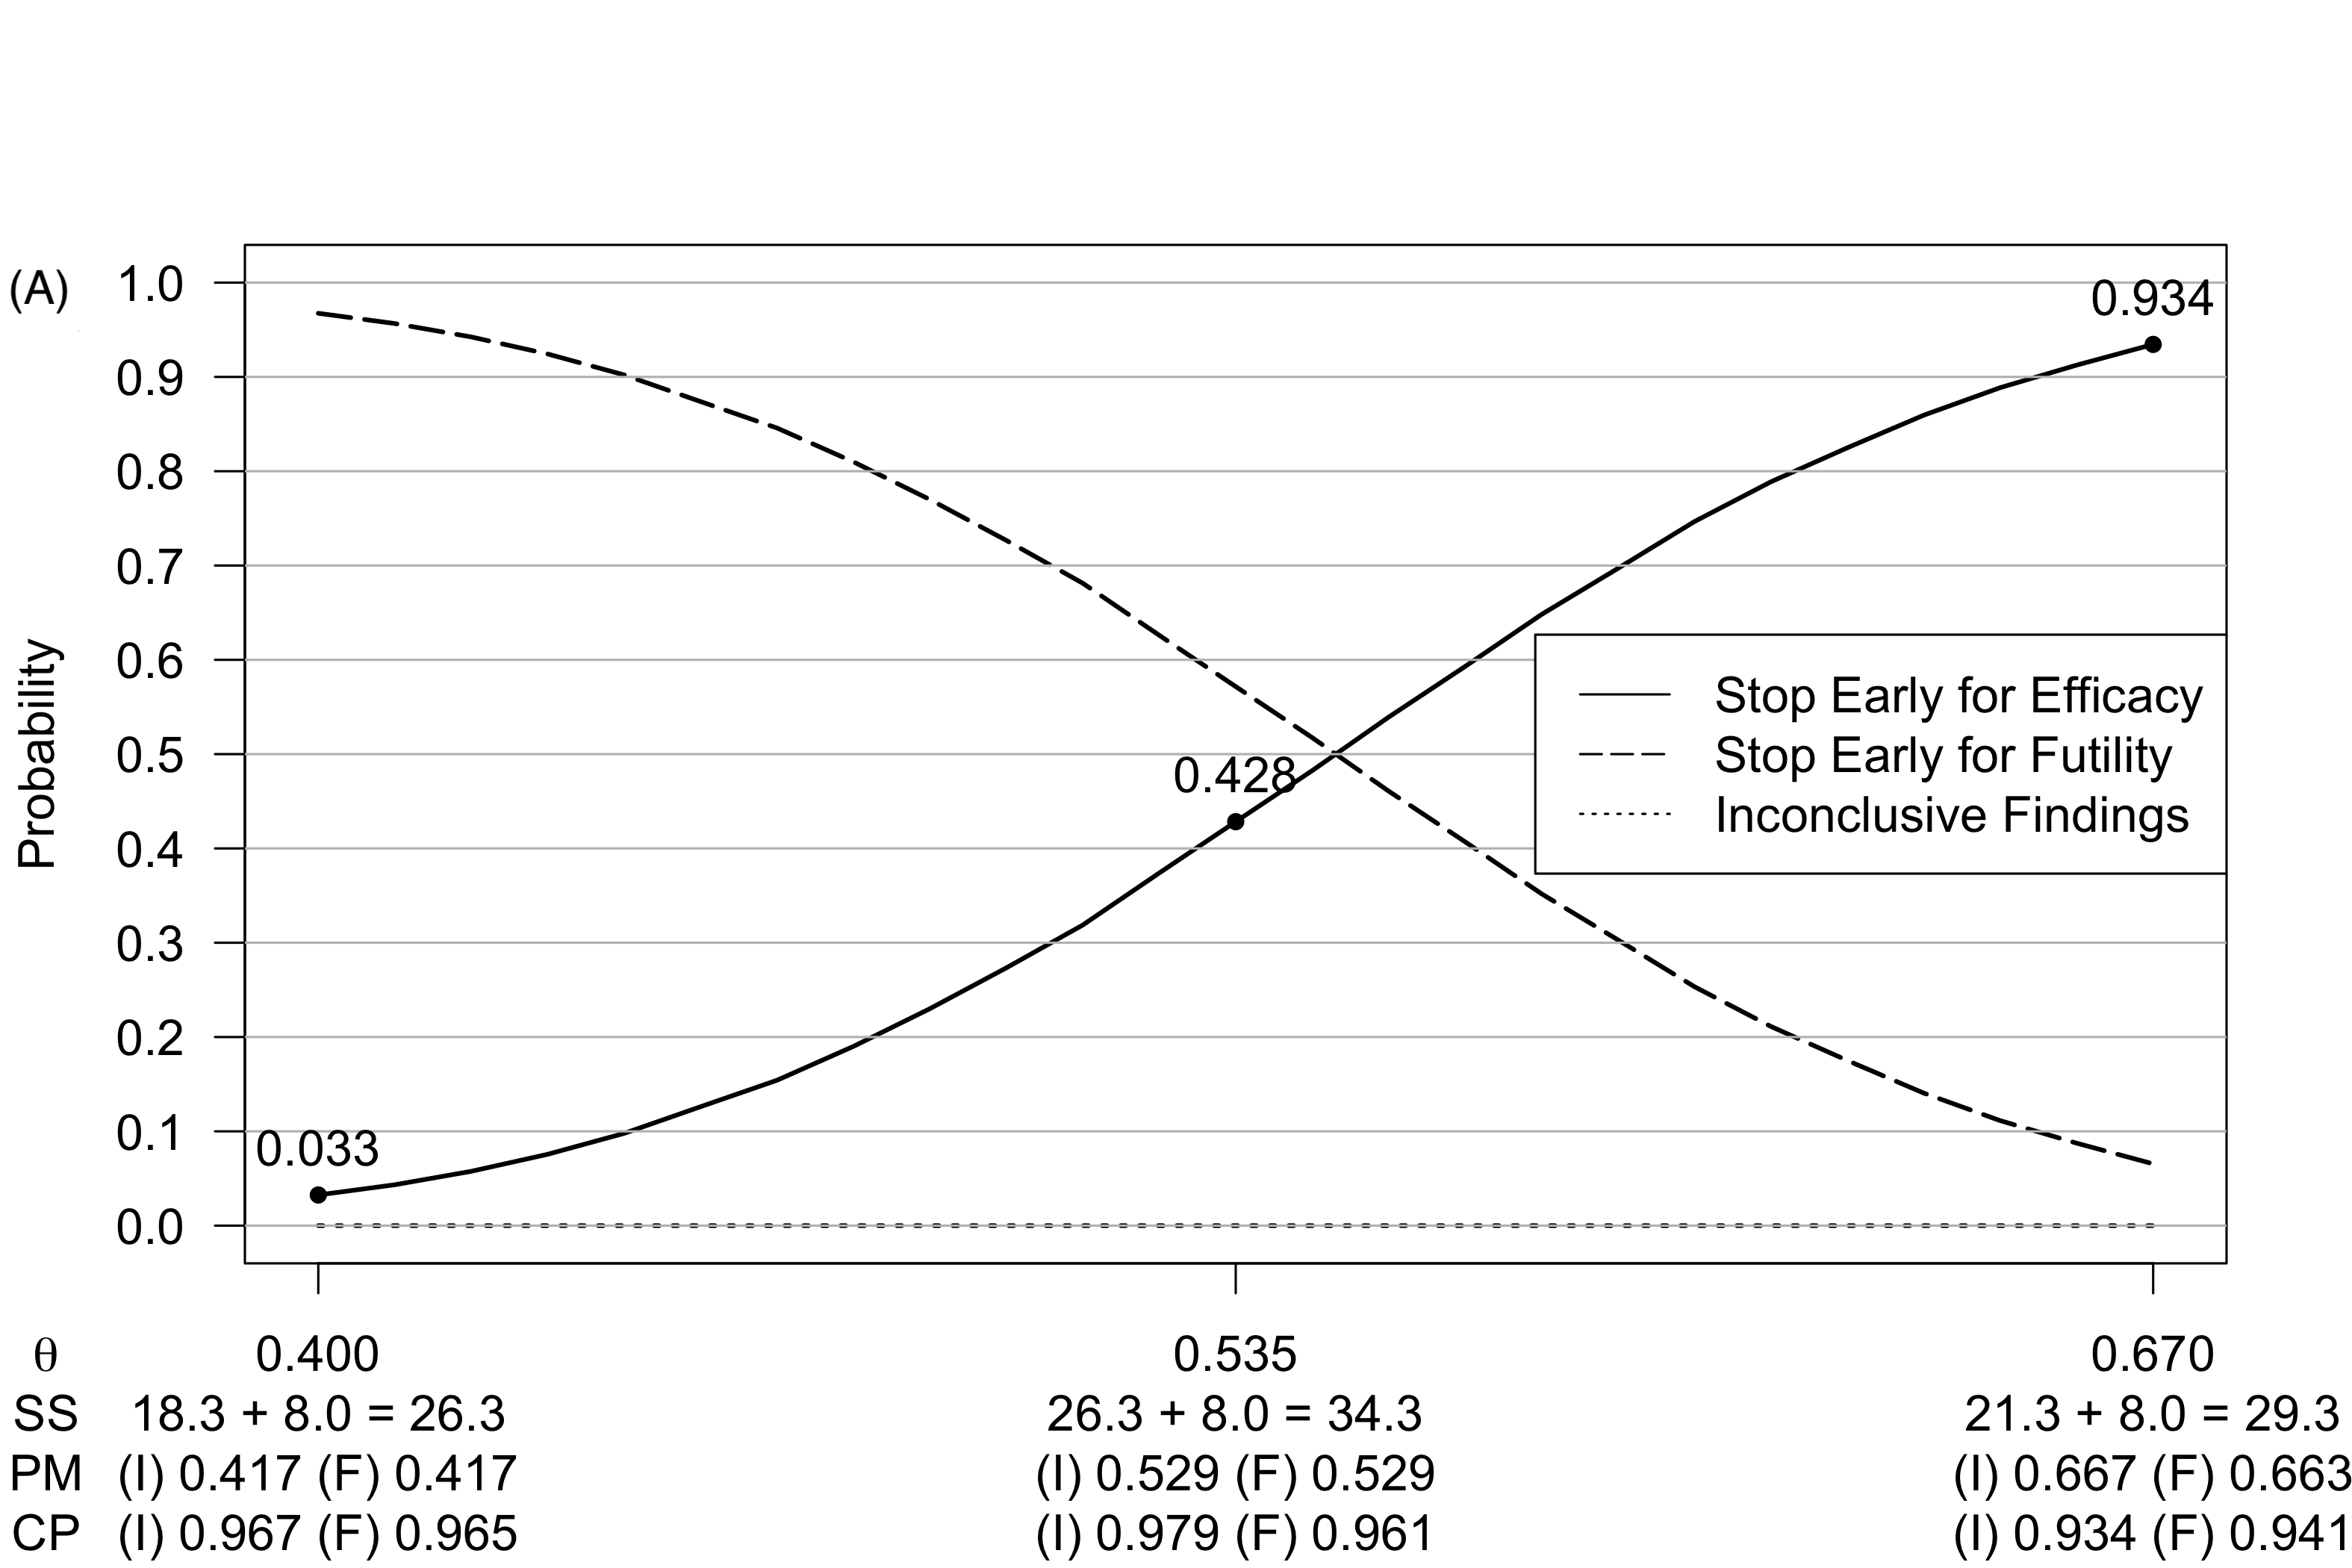
\includegraphics[width=7in]{P:/Bayesian-Sequential-Monitoring/00-paper/FIGURES/figureS2c.png}
    \caption{Caption text 1}
  \end{subfigure}
  \begin{subfigure}{7in}
    \centering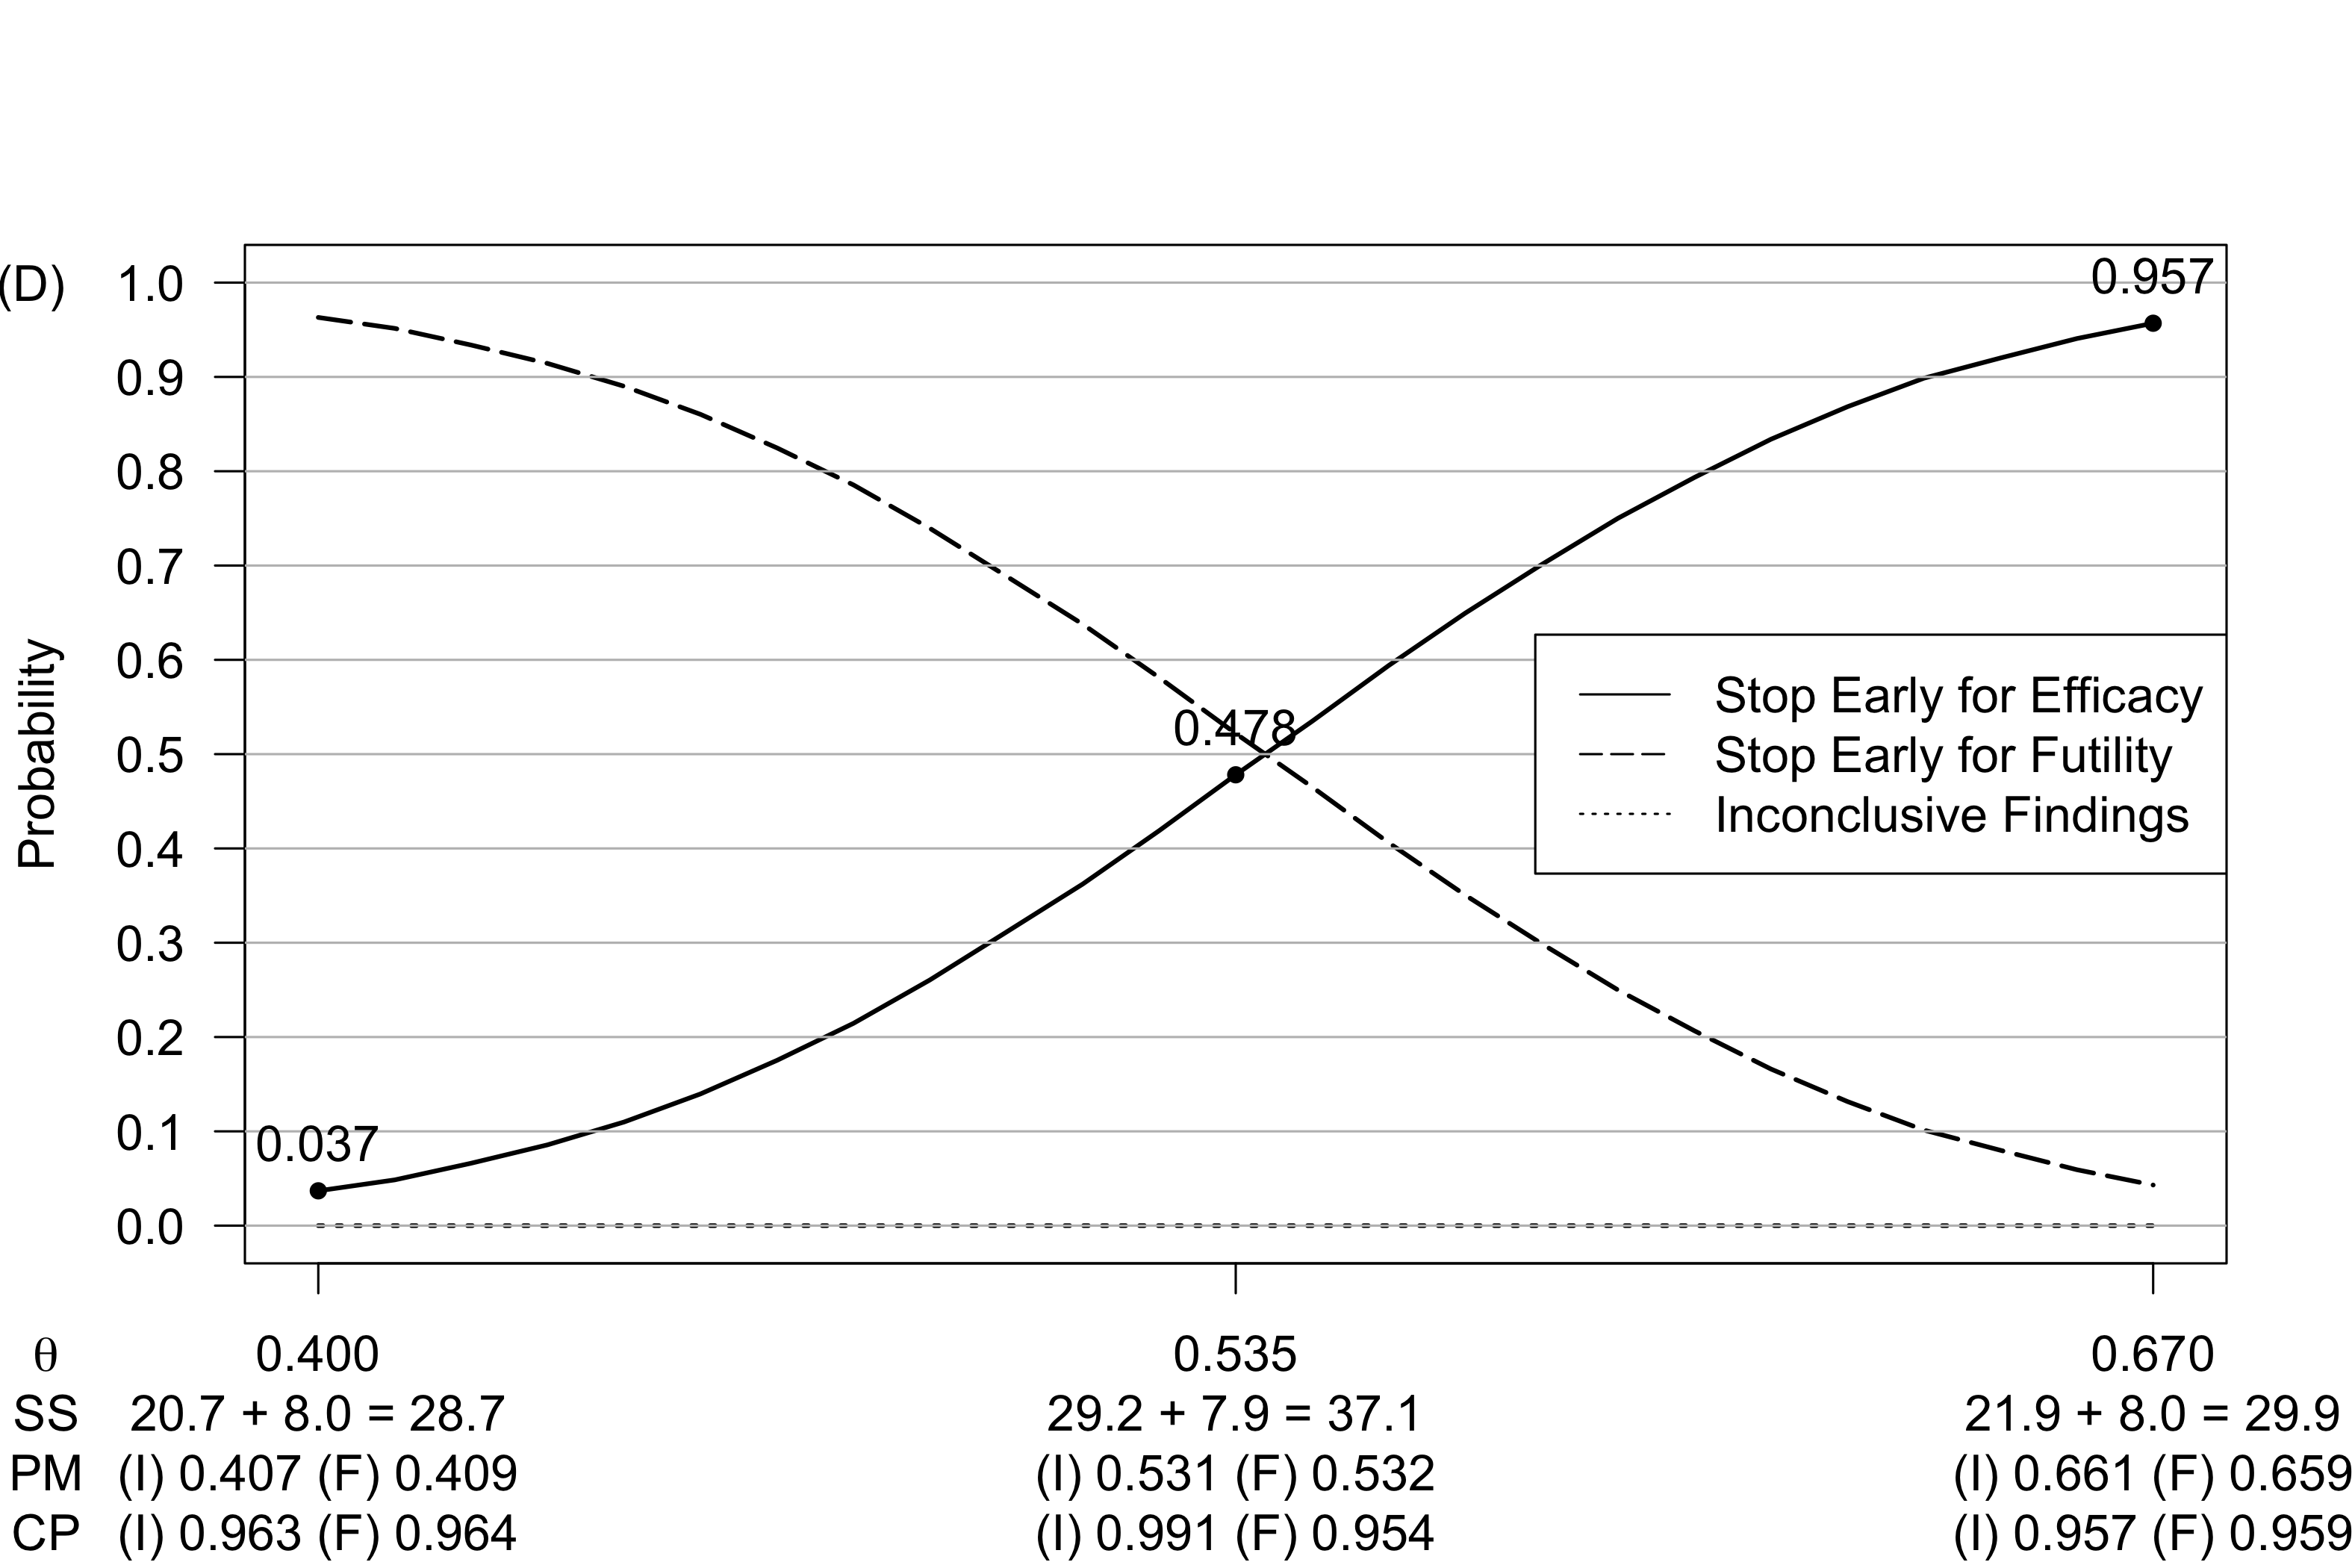
\includegraphics[width=7in]{P:/Bayesian-Sequential-Monitoring/00-paper/FIGURES/figureS2d.png}
    \caption{Caption text 2}
  \end{subfigure}
\end{figure}

\section{BibTeX}

 \bibliographystyle{agsm}
 \bibliography{./References}		

\end{document}
